\documentclass{sig-alternate-10pt}
\usepackage{color}
\usepackage{colortbl}
\usepackage{graphicx}
\usepackage{setspace}
\usepackage{multirow}
%\doublespacingjj
\hyphenation{sub-scribe sys-tems}
\newcommand\note[1]{\textcolor{red}{$=>$ #1}}

\begin{document}

\CopyrightYear{2010} % Allows default copyright year (200X) to be over-ridden - IF NEED BE.

\title{BGPmon Version7}
\subtitle{Implementation and Technical Specification}
\numberofauthors{1} 
\author{
\alignauthor
He Yan, Kevin Burnett, Mikhail Strizhov, Dave Matthews and Daniel Massey\\
       \affaddr{Colorado State University}\\
       \affaddr{Computer Science Department}\\
       \affaddr{Fort Collins, Colorado, USA 80523}\\
       \email{[yanhe,burnet,strizhov,dvmtthws,massey]@cs.colostate.edu}
}
\maketitle

\begin{abstract}
This paper presents a new system, called BGPmon, for monitoring the Border Gateway Protocol (BGP).  BGP is the routing protocol for the global Internet.  
Monitoring BGP is important for both operations and research; a number of public and private BGP monitors are deployed and widely used.  
%Most monitors use open source routing toolkits to capture and log updates.  
%However, the routing toolkits add unnecessary complexity to the monitor by implementing routing polices, storing RIB tables, forwarding packets and so forth.   Furthermore, most routing toolkits do not easily facilitate real-time access, do not scale to vast numbers of peers, and are not easily extended.
These existing monitors typically collect data using a full implementation of a BGP router. In contrast, BGPmon eliminates the unnecessary functions of route selection and data forwarding to focus solely on the monitoring function.   
BGPmon uses a publish/subscribe overlay network to provide real-time access to vast numbers of peers and clients. 
%Using features such as route refresh, 
All routing events are consolidated into a single XML stream.  
XML allows us to add additional features such as labeling updates to allow easy identification of useful data by clients.  
Clients subscribe to BGPmon and receive the XML stream, performing tasks such as archiving, filtering, or real-time data analysis.  
BGPmon enables scalable real-time monitoring data distribution by allowing monitors to peer with each other and form an overlay network to provide new services and features without modifying the monitors.  
\end{abstract}

\section{Introduction}
\label{sec:intro}

BGPmon Test Framework  is a collection of software and testing data that tests BGPmon components by running it under various conditions. BGPmon Test Framework has multiple test units that run specific tests and also provide a way to monitor and  analyse results. 

BGPmon Test Framework has following objectives: 
\begin{itemize}
  \item{It should help in automation of BGPmon testing process.}
  \item{It should increase development productivity.}
  \item{It should increase quality of BGPmon components and application.}
  \item{Test units need to include conditions that BGPmon application meet in production environment and conditions that difficult to simulate.}
  \item{It should generate human-readable test reports.}
\end{itemize}

BGPmon Test Framework is designed for  people who interested in testing newly developed or existing components in BGPmon application. BGPmon Test Framework might be interested to people who wants to verify that each particular piece of code that has been written performs the function that it is designed to do. Thus, the audience or users for this document are software developers and quality
managers.
  
%Overall, 
%this  document describes BGPmon Test Framework and its test units. 
%this paper is organized as follows. Section \ref{sec:descr} talks about Test Framework test units. Section \ref{sec:essentials} describes Test Framework essentials: where and how  to start using Test Framework, log options in Test Framework and others.  Section \ref{sec:ipv4peer} describes \emph{IPv4 Peering Test Unit}. It include test unit objectives, unit launch and results reporting.  Section \ref{sec:ipv6peer} introduces \emph{IPv6 Peering Test Unit}. Section \ref{sec:mrt} describes \emph{MRT Module Test Unit} that designed to test MRT module in BGPmon application.  Section \ref{sec:chain} discuss \emph{Chain Modulte Test Unit}. Section \ref{sec:webclient} describes \emph{WebStat Client Test Unit} that tests XML module in BGPmon and provide visual HTML report. 

%Testing framework consist of several test units that are designed for testing BGPmon components and modules.
% like IPv4 and IPv6 peering modules, MRT and Chain modules, WebStat client. 


  
%what is the purpose of the test framework?  
%why we are producing this test framework?

%who is the intended audience?   

%what can they do with it?   

%why would they be using it?


\subsection{BGPmon Test Framework Overview}
\label{sec:current}

%\subsection{Test Units}
\begin{figure}
\centering
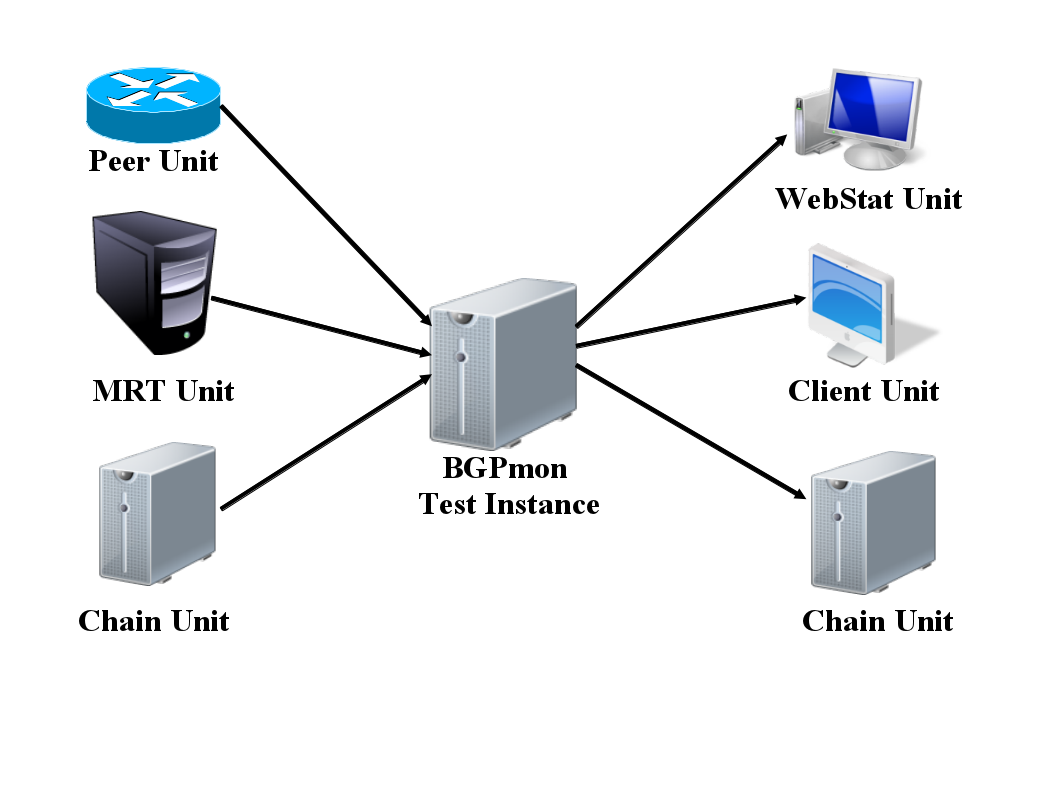
\includegraphics[scale=0.40]{figs/BGPmon-framework-design.png}
\caption{An overview of BGPmon Test Framework architecture.}
\label{designfig}
\end{figure}

Figure \ref{designfig} shows ideal setup of  BGPmon Test Framework that has 7 components.   Test Framework is designed in the way that it tests functionality of  modules in BGPmon application.  BGPmon test instance that shown in the center of the figure  has 3 distinct types of input: \emph{Peer}, \emph{MRT} and \emph{Chain} units.  First, \emph{Peer} unit, sends BGP messages over the BGP peering session.   Second, \emph{MRT} unit, provide BGP messages in MRT format.  \emph{Peer} unit is different from \emph{MRT} unit in the way that \emph{Peer} sends BGP messages that are collected directly from a peer, while \emph{MRT} unit provide data from indirect peer through third party. \emph{Chain} logical unit sends BGP messages in a form of XML messages. \emph{Chain} unit is different from \emph{Peer} and \emph{MRT} because it provides messages from other BGPmons. \emph{Peer}, \emph{MRT} and \emph{Chain} units are shown on the left part of Figure \ref{designfig}.   
BGPmon test instance has three types of output: \emph{WebStat}, \emph{Client} and \emph{Chain} units. All 3 units receive XML messages from BGPmon test instance but use it in different way. \emph{WebStat} unit use XML feed to  generate status report about \emph{Peer}, \emph{MRT} and \emph{Chain} units. \emph{Client} is a setup that used for analysis of XML update messages. \emph{Chain} unit is a separate unit that use XML messages to create a mesh network of BGPmons. \emph{WebStat}, \emph{Client} and \emph{Chain} units are shown on the right part of  Figure \ref{designfig}. 

In order to run over IPv4 and IPv6 communication protocols, design of BGPmon Test Framework need be to be updated by introducing IPv4 and IPv6 units in input and output to BGPmon test instance. Thus, 3 types of input (\emph{Peer}, \emph{MRT} and  \emph{Chain}) and 3 types of output (\emph{WebStat}, \emph{Client} and \emph{Chain})  need to have IPv4 and IPv6 units.  For instance, \emph{Peer} logical unit includes \emph{IPv4 Peer} and \emph{IPv6 Peer} testbeds, \emph{MRT} unit have \emph{IPv4 MRT} and \emph{IPv6 MRT} and so forth.  Thus, BGPmon Test Framework presents complete picture of a testbed that designed to support all distinct types of input and output in BGPmon application.

% Today BGPmon application has support of both IPv4 and IPv6 communication protocols and Test Framework include separate IPv4 and IPv6 logical pieces for each of input sources. Figure \ref{designfig}  shows 6 logical pieces on the left: \emph{IPv4 and IPv6 Peers}, \emph{IPv4 and IPv6 MRTs} and \emph{IPv4 and IPv6 Chains}.   On the right side  of the figure,  Test Framework has elements that receive data from BGPmon application.  It includes installation of \emph{IPv4 and IPv6 WebStat clients}, \emph{IPv4 and IPv6 Generic Clients} and \emph{IPv4 and IPv6 Chains}.    Each logical units  has its own and unique goals to test different components of BGPmon test instance.    

\subsection{Current BGPmon Test Framework Setup}

\begin{figure}
\centering
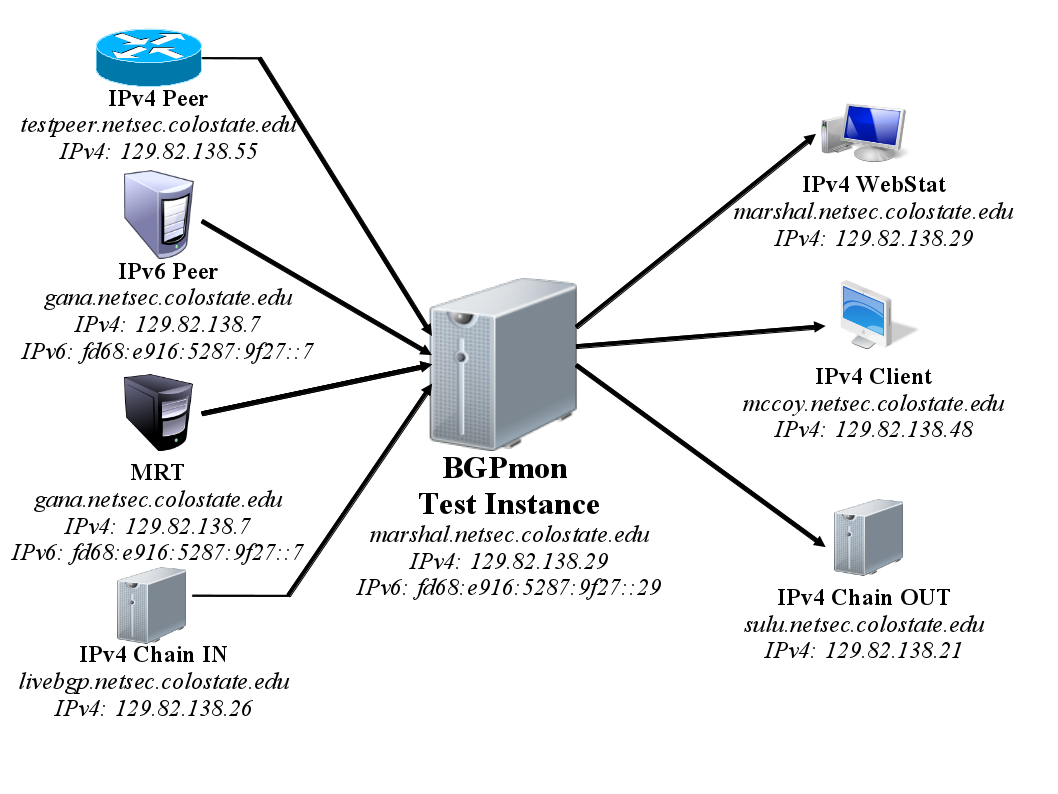
\includegraphics[scale=0.40]{figs/BGPmon-framework-current.png}
\caption{An overview of BGPmon Test Framework architecture.}
\label{currentfig}
\end{figure}

This section describes installation of BGPmon Test Framework and its current status.  Figure \ref{currentfig} shows existing installation and units. BGPmon test instance is installed on \emph{marshal.netsec.colostate.edu} with \emph{129.82.138.29} IPv4 address and \emph{fd68:e916:5287:9f27::101} IPv6 address.        Due to lack of   available equipment and full IPv6 connectivity, existing BGPmon Test Framework setup has limitations and not all logical pieces present in a current installation. 

In Figure \ref{currentfig}, \emph{Peer} unit includes two testbeds: \emph{IPv4 Peer} and \emph{IPv6 Peer} units. \emph{IPv4 Peer} is a setup of Cisco Router and BGPmon instance.  Cisco Router has  \emph{testpeer.netsec.colostate.edu} hostname and \emph{129.82.138.55} IPv4 address.  Despite that this scheme  is designed to test IPv4 peering functionality, it also tests BGPmon  components to receive and process  BGP update messages. Also, \emph{IPv4 Peer} unit is designed to test  BGPmon's efficiency to work with BGP capabilities. \emph{IPv6 Peer} unit is a setup of Quagga Routing Suite software and BGPmon instance. \emph{IPv6 Peer} unit has same goals as \emph{IPv4 Peering}, but it designed to run over IPv6 connectivity.  Quagga software is configured on \emph{gana.netsec.colostate.edu} with two IP addresses: \emph{129.82.138.7} is IPv4 address and \emph{fd68:e916:5287:9f27::101} IPv6 address.  Section \ref{sec:peer} has detailed information about \emph{IPv4 Peer} and \emph{IPv6 Peer} unit goals,  configuration defaults and other. 

\emph{MRT} logical unit includes \emph{IPv4 MRT} testbed that is setup of MRT software and BGPmon test instance.  MRT software is an application that runs on \emph{gana.netsec.colostate.edu} with \emph{129.82.138.7} IP address. MRT application is designed to provide routing data as a third party. In particular, it provides routing data from existing route collectors like Oregon RouteViews project, but it could be used to give routing data from any other MRT source provider.  Section \ref{sec:mrt} has  more details about \emph{IPv4 MRT} unit.

\emph{Chain} logical unit has \emph{IPv4 Chain IN} and \emph{IPv4 Chain OUT} units. First, \emph{IPv4 Chain IN} unit is configuration of BGPmon application that provide stream of table and update messages in a form of XML messages.  \emph{IPv4 Chain IN} runs it on \emph{livebgp.netsec.colostate.edu} and table and update messages are available on ports \emph{50001} and \emph{50002} respectively.  \emph{IPv4 Chain OUT} is setup of BGPmon application that configured to receive XML feed from BGPmon test instance. \emph{IPv4 Chain OUT} is configured on \emph{sulu.netsec.colostate.edu} with \emph{129.82.138.21} IPv4 address.  Thus, \emph{IPv4 Chain IN}, BGPmon test instance and \emph{IPv4 Chain OUT} creates a mesh of BGPmons.  Overall, \emph{IPv4 Chain} that includes both \emph{IPv4 Chain IN} and \emph{IPv4 Chain OUT} units  tests BGPmon's Chain module functionality to create a mesh network of BGPmons, ability of receive and process XML data streams. Section \ref{sec:chain} describes details of this test unit. 

There are 3 types of output that are shown on the right of Figure \ref{currentfig} \emph{WebStat} unit, \emph{Client} unit and \emph{Chain} unit.  

\emph{WebStat} unit include \emph{IPv4 WebStat} testbed that has WebStat software and BGPmon instance.  WebStat software is application that runs on \emph{marshal.netsec.colostate.edu}. WebStat application consist of two components, first, \emph{StatClient} and second, \emph{WebGen}. \emph{StatClient} is application that connects to BGPmon instance and store extracted XML feed in a file system. \emph{WebGen } is unit that generates HTML report that makes summary of configured inputs to BGPmon test instance.  Section \ref{sec:webclient} includes testbed description, test unit goals and others. 

\emph{Client} unit has \emph{IPv4 Client} testbed that is setup of Client software and BGPmon test instance. Client software is application that is configured on \emph{mccoy.netsec.colostate.edu} with \emph{129.82.138.48} IPv4 address. Client software is designed to receive and print XML update messages in a human readable format. Section \ref{sec:client} describes \emph{IPv4 Client} in details. 
 

%Overall, the nature of BGPmon Test Framework Test Units could be divided in two groups: \emph{producers} and \emph{consumers}. \emph{Producers} group include \emph{IPv4 Peering Test Unit}, \emph{IPv6 Peering Test Unit},  \emph{MRT Module Test Unit}  and \emph{Chain Module Test Unit}. \emph{Producers} are the entities that provide data into the system. \emph{Consumers} group include \emph{WebStat Client Test Unit} because this test unit is designed to receive data and analyse it. Thus, the flow of the BGPmon Test Framework could be described in a way that each unit test in \emph{Producers} could be verified with \emph{Consumers} test unit.  For instance, running \emph{MRT Module Test Unit} will generate stream of MRT data that could be easily monitored and analysed using \emph{WebStat Client Test Unit}. Same flow model could be applied to any other test unit in \emph{Producers} group.

\subsection{BGPmon Test Framework Essentials}
\label{sec:essentials}

This sections describes Test Framework Essentials that are important before running any test units. 

Test Framework is configured on \emph{marshal.netsec.colostate.edu}. To get an access to \emph{marshal.netsec.colostate.edu} users of framework need to have access to \emph{bgpmoner} account on \emph{marshal.netsec.colostate.edu}. \emph{bgpmoner} account has all necessary privileges in a system to run or execute Test Framework.  

\subsubsection{BGPmon Launch}

To start using BGPmon Test Framework, BGPmon application has to be launched. To start BGPmon, run following  \emph{init.d} script in a terminal:

\begin{verbatim}
$ sudo /etc/init.d/bgpmon start
\end{verbatim}

This command launches BGPmon application in a background.

To stop using BGPmon Test Framework, stop  BGPmon application:

\begin{verbatim}
$ sudo /etc/init.d/bgpmon stop
\end{verbatim}

\subsubsection{BGPmon Source Code}
Source code of BGPmon application is installed in home directory of \emph{bgpmoner} in following directory:

\begin{verbatim}
/home/bgpmoner/Development/bgpmon-dev
\end{verbatim}

\subsubsection{BGPmon Init.d Script}

Before start using BGPmon application, structure of \emph{init.d} script should be discussed.   \emph{/etc/init.d/bgpmon} script has following definitions:

\begin{verbatim}
BGPMON_EXEC=/usr/local/bin/bgpmon 
CONFIG_FILE=/usr/local/etc/bgpmon_config.txt
PIDFILE=/var/run/bgpmon.pid
ARGS="-d -c $CONFIG_FILE -s -l 7"
\end{verbatim}

\emph{BGPMON\_EXEC} is variable that specifies location of BGPmon executable file. \emph{CONFIG\_FILE} shows location of configuration file that store BGPmon settings.  \emph{PIDFILE} is variable that points to process ID location that is used by \emph{init.d} script. Lastly, \emph{ARGS} is list of command line arguments.   BGPmon application starts with parsing the command line arguments. There are few simple command line arguments that could be specified. In example above, BGPmon uses \emph{-d} to run in daemon world,  \emph{-c \$CONFIG\_FILE} to load default configuration file, \emph{-s} to print log messages to stdlog, \emph{-l 7} defines the log level . In order to debug problems in BGPmon, last two options worth  discussion.

User of the framework may configure BGPmon log functionality to use  \emph{stdout} or \emph{syslog} modes.  First, \emph{stdout mode}, configures BGPmon to run  in an interactive mode that sends all messages to standart output (i.e. terminal).  To enable this option in \emph{init.d}, change \emph{ARGS} line to following:
\begin{verbatim}
ARGS="-d -c $CONFIG_FILE -i -l 7"
\end{verbatim}

Second, \emph{stdlog mode}, configures BGPmon to run in log mode that sends all messages to a file that specified in syslog. \emph{-s} command line argument enables \emph{syslog mode} and \emph{marshal.netsec.colostate.edu} prints log messages to \emph{/var/log/messages} file. To enable \emph{init.d} script use \emph{stdlog mode} use following configuration in \emph{ARGS}:
\begin{verbatim}
ARGS="-d -c $CONFIG_FILE -s -l 7"
\end{verbatim}

BGPmon application  supports different log levels.  \emph{Init.d} script  \emph{/etc/init.d/bgpmon} uses option \emph{-l} with  log value of 7 (\emph{Debug}) and it includes  log values from 0 to 7 (\emph{Emergencies, Alerts, Critical Errors, Errors, Notices, Information, or Debug}). \emph{Debug} provide complete picture of messages that BGPmon application generates. However,  users of framework may configure BGPmon Test Framework log reports to use different levels. This option provides different view of generated logs. For instance, if user  wants to run framework with lower log level like 4 (\emph{Warning}), it need to run \emph{init.d} script with specified log level value. To launch Test Framework with \emph{Warning} log level, change \emph{ARGS} line in \emph{init.d} script to:
\begin{verbatim}
ARGS="-d -c $CONFIG_FILE -s -l 4"
\end{verbatim}

In general, user of framework is free to set any log level value ranging from 0 to 7 by changing \emph{ARGS} value:
\begin{verbatim}
ARGS="-d -c $CONFIG_FILE -s -l logvalue"
\end{verbatim}

%I'm a new developer on BGPmon so I'm looking for you to explain DEBUG to me.       Yes,  I could uncomment this and get something....    not clear why I want to do that?  
%where is this DEBUG?   does setting it one module set it everywhere?
%do want DEBUG in the log or to stdout?
%could I do multiple DEBUG at the same time?
%Jason said in the meeting,  just set DEBUG globally.   is that good or bad?  why?
%am I expected to add my own DEBUG statements as I test?  (answer there is absolutely yes.   does this %document give me enough to understand that?

To truly understand the work flow of components in BGPmon Test Framework, BGPmon application supports modular debugging.  This feature includes critical  messages that are produced by each component during the execution of BGPmon. In order to get the right picture of how components in BGPmon work and communicate between each other, user may enable \emph{DEBUG mode}.  Every source file  in BGPmon home directory has the following macro at the beginning  (after  system libraries linking): 
\begin{verbatim}
//DEFINE DEBUG
\end{verbatim}

Functions in BGPmon components use \emph{controlled text} to print values to stdout. For example:

\begin{verbatim}
#ifdef DEBUG
  debug(__FUNCTION__, "New session with id %d for peer %d", i, peerID);
#endif
\end{verbatim} 

This block is called a \emph{conditional block}. \emph{Debug()} is \emph{controlled text} that will be executed in the output of the preprocessor if and only if \emph{DEBUG} macro is enabled. Most of the functions in BGPmon have at least one conditional block that is wrapped around in  \emph{DEBUG}  macro. 

There are many variants how user can use \emph{DEBUG} macro.  For example, to see  work flow messages from all components, user may recompile BGPmon source code with "-DDEBUG" option. This will enable \emph{DEBUG mode} in each component in BGPmon application.  In this example,  every component would start sending very large amount of log messages to log output and it may create difficulty in understanding and debugging founded problems in BGPmon code.  Instead,  user may uncomment \emph{DEBUG} macro in specific modules. For instance, to enable \emph{DEBUG mode} in \emph{Peering} module in BGPmon application, uncomment \emph{DEBUG} macro :
\begin{verbatim}
//DEFINE DEBUG
\end{verbatim}
to
\begin{verbatim}
DEFINE DEBUG
\end{verbatim}

in each \emph{*.c} source file in \emph{Peering} directory in BGPmon source home directory. To see debug messages, user need to recompile source code and install executable files in a system. In this example,  all \emph{conditional blocks}  that defined in Peering module will be executed.  Also, \emph{DEBUG mode}  functionality could be enabled in any module or groups of modules to debug the problems in BGPmon application. 

However, some users may feel that \emph{DEBUG mode} is not sufficient or  there are too little messages in the output. They can create their own conditional blocks.  Simply,  include conditional block in a function that require additional debugging in source file:
\begin{verbatim}
#ifdef DEBUG
  debug(__FUNCTION__, "Test values are  %d and  %d", value1,  value2);
#endif
\end{verbatim}  

In this example, \emph{debug()} function will print the name of the function (where this block was executed) and two integer values \emph{value1} and \emph{value2} . 

%\subsubsection{BGPmon: Debugging Problems}
%User of Test Framework can debug BGPmon application with set of available tools like \emph{gdb} and %\emph{valgrind}. Those tools can automatically detect memory management problems, threading bugs and %profile your programs in detail.

or what another program was doing at the moment it crashed.
\subsubsection{Test Framework Misconfigurations}

In order to give a complete picture of BGPmon Test Framework Essentials, user need to know about possible misconfigurations in a testbed and further consequences.  Test units in Test Framework might be  configured with any test settings including valid or invalid values. Any misconfigurations  might brake not only test framework setup, but it may affect already working systems.  For example, user may configure to send set of custom MRT update files to \emph{bgpdata.netsec.colostate.edu} hostname  that is not shows on Figure \ref{currentfig}. Results would be tragic, \emph{bgpdata.netsec.colostate.edu} will  provide incorrect data to end clients and it will cause a lot of problems to managers of BGPmon project.  In order to prevent such events, user of framework need to use resources (machines, routers, etc) that are   that are shown on Figure \ref{currentfig} only.   Any usage of other resources is \textbf{strictly forbidden} or it has be discussed with developers and managers of BGPmon project.

%Shell script \emph{/etc/init.d/bgpmon\_startup\_debian.sh} allow user to start and stop BGPmon process. When user run script with ”start” option, it will put BGPmon process in daemon world. Option "stop" with script  terminates BGPmon process using \emph{/var/run/bgpmon.pid} process ID.




%\subsection{Configuration file}
%BGPmon instance load default configuration file \emph{/usr/local/etc/bgpmon\_config.txt}. This file contains internal settings for BGPmon and configuration for BGPmon modules. This file is used every time when user starts or restart BGPmon.  

%\subsection{Logging}
%BGPmon uses \emph{/var/log/messages} file to write all info and debug messages.  

%\subsection{Configuration and Source Code}
%In order to configure BGPmon user has to be logged to \emph{marshal.netsec.colostate.edu}.  BGPmon source code is located in \emph{/home/bgpmoner/Development/bgpmon-dev} directory. To install or reinstall BGPmon, user need to run \emph{./configure \&\& make \&\& sudo make install}.
\section{BGPmon: New Monitoring System}
\label{sec:main}

Open source routing software that is currently used as a collector typically implements a full routing protocol, including receiving routes, applying policies, setting forwarding states, and announcing routes to peers. 
These activities involve considerable complexity, but none of these actions are needed to be collector. 
A collector simply needs to receive and log routes. 
Our new collector design focuses on a narrow set of data collection functions. 
By focusing on the collection functionality and eliminating unnecessary tasks, the new collector is able to scale up and support more peer routers while making the data available in real-time to a potentially vast number of clients. 

%\begin{figure*}[t]
%\centering
%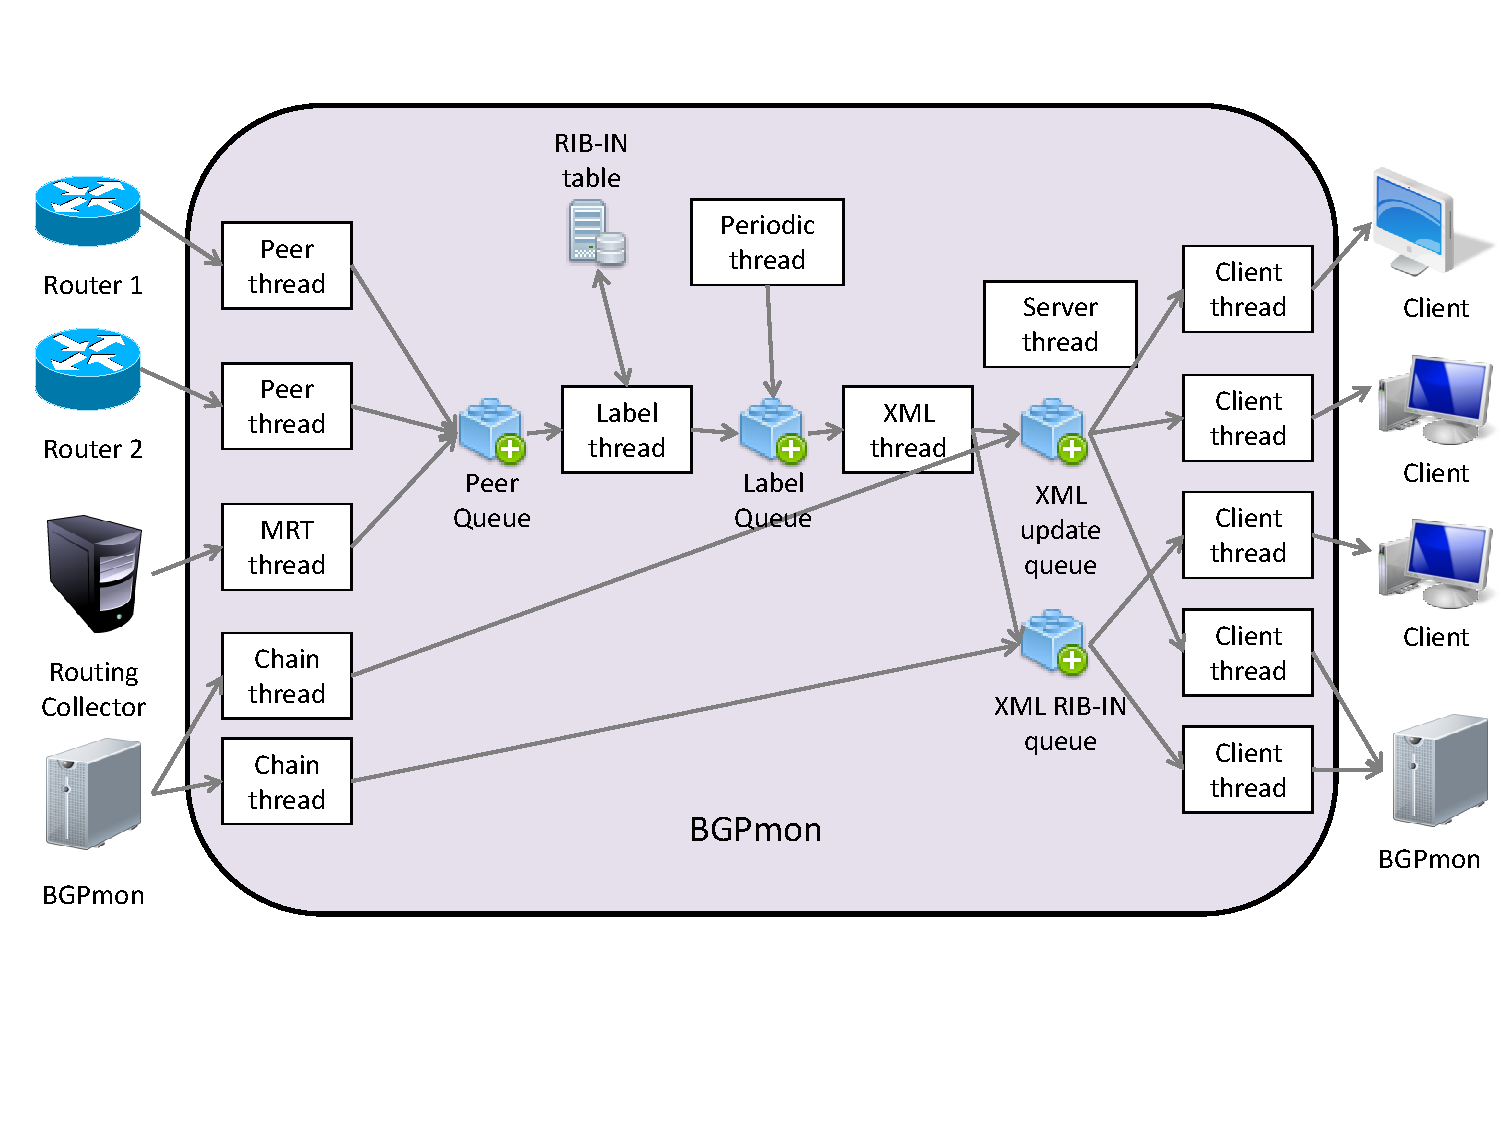
\includegraphics[scale=0.50]{figs/BGPmon-architecture.pdf}
%\caption{BGPmon architecture.}
%\label{architecturediagram}
%\end{figure*}

To support hundreds of peer routers and clients, one would like to scale out across multiple systems by adding more collectors and distributing the services. 
At the same time, a client should see a single monitoring service and be unaware that the implementation of the service may be done through multiple collectors. 
Our approach is based on publish/subscribe overlay networks that consist of brokers, publishers, and subscribers. 
The brokers form the overlay network, allowing publishers to send event streams to the overlay network and allowing subscribers to receive event streams from the overlay network. 
Publishers and subscribers interact only with brokers, not with each other, allowing the overlay network to insulate publishers and subscribers from each other. 

To improve fault tolerance, multiple brokers may monitor the same or different peers in an AS, yet appear to a client application as a single subscription. 
This allows critical applications to continue to receive event streams in the case of a failure of a peer, monitor, or broker. 
Our system implementation begins with BGPmon, a simple monitoring system now available that incorporates all three functions: publish, broker, and subscribe. 


%\section{Configuration Module}
\label{sec:config}

Configuration of BGPmon is entirely via command line interface which is very similar to a cisco router. Internally all the configurations will be stored in a XML file which can be loaded later. The configuration of a module corresponds to a  part of the XML file. In a high level, configuration module builds a bridge between main program and all the other modules in oder to facilitate the configuration management. 
More specifically, configuration module mainly consists of 3 parts.
First configuration module provides a facade to main program that allows it to read, save and backup XML configuration file without knowing the details of other modules . Secondly configuration module provides some XML utility functions to other modules as each of them needs the same set of functions to read configuration from XML file and save configuration into XML file. At last, configuration module is also a centralized place to define the XPaths of  all the configuration. 
  
  
 \subsection{Read, Save and Backup XML Configuation File} 
Configuration module provides the following 3 functions to main program:
 \begin{itemize}
 	\item{\emph{ readConfigFile: } This facade function is called by main program to load the configuration into memory from XML file. Instead of direct reading the XML configuration file it delegate reading functions to each module. In other words, each module provides a reading configuration function to load its own configuration from XML file and the facade function just needs to call these read functions in order to load all the configuration.
	If the XML configuration file is corrupted, this function will try to load as much as possible into memory and return a error code .}
	\item{\emph{ saveConfigFile:} This facade function is called by main program and login module to write the configuration from memory into XML file. Similar to \emph{ readConfigFile}, it doesn't directly write the configuration into XML file. Each module provides a writing configuration function to write its own configuration into XML file and this facade function just calls them one by one.}   
	\item{\emph{ backupConfigFile:} This function is called by main program to back up the current configuration file. It is called typically when the current configuration file is corrupted.}
	We described in details how main program uses the 3 functions in section \ref{sec:main}.
\end{itemize}  
 
  \subsection{XML Utility Functions} 
Configuration module provides a couple of get and set functions to read and write XML file.  The caller of these functions needs to pass in the XPath to locate a particular configuration item.
These get functions can return the configuration item in a specified data type and check the value against the specified conditions. For example, the caller can specify to get a configuration item in integer and check if the value is between 0 and 10. If this configuration item in XML file cannot be converted to a integer or its value is larger than 10, a error code will be returned.
 
  \subsection{XPath Definitions} 
  Each module needs to define a bunch of XPaths in order to read its own configurations from XML file.  For example, for the clients management module it configurations look like this:
     \begin{verbatim}
	<BGPmon>
    <CLIENTS>
       <LISTEN_ADDR>ipv4loopback</LISTEN_ADDR>
       <LISTEN_PORT>50001</LISTEN_PORT>
       <ENABLED>0</ENABLED>
       <MAX_CLIENTS>10000</MAX_CLIENTS>
    </CLIENTS>
	</BGPmon>
\end{verbatim}
As a result, clients management module needs to define 4 XPaths for the 4 items: LISTEN\_ADDR, LISTEN\_PORT, ENABLED and MAX\_CLIENTS. In order to get the 4 values,  clients management module needs to call the get functions mentioned before and pass in the XPaths. The XPath definitions of all modules can be found in Config\/configdefaults.h.
  
  
  \subsection{Design Philosophy} 
  As each module has the best knowledge of its own con�guration, our design divides the entire con�guration of BGPmon into a couple of small pieces according to the division of modules. Each module only handles it own piece. In this way, the changes of con�guration will be localized inside one module and none of them will be exposed to main program or other modules. XML utility functions are de�ned here as most of modules need them to handle the XML �le. Also in order to manage all the XPaths of modules e?ciently, they are centralized stored in the con�guration module. The last design issue here is about default con�guration. There are 2 reasons why we need this default con�guration.
   \begin{itemize}
 	\item{ It includes the minimal set of con�guration to start BGPmon for this �rst time. For 	example, the command line interface needs a default enable password and a default port to
	listen on even if there is no con�guration yet.}
	\item{ It provides the defaults for all the optional con�guration. For example, the BGP
	version of peer con�guration is optional and the default value will be used if it is not speci�ed by the user.}   
\end{itemize}  

The default con�guration of BGPmon can be found in site defaults.h. It can be changed by editing this �le and then recompile BGPmon. And default con�guration will be overwritten by the con�guration via command line interface.

%  As each module has the best knowledge of its own configurations, our design divides the entire configurations of BGPmon into a couple of small pieces according to the division of modules. Each module only handles it own piece.
%  In this way, the changes of configurations will be localized inside one module and none of them will be exposed to main program or other modules. 
%  XML utility functions are defined here as most of modules need them to handle the configurations in XML file. Also in order to manage all the XPaths of modules efficiently, they are  centralized stored in the configuration module.  
%    
%The BGPmon configuration parameters are divided into four classes.   First,  \emph{Peering Parameters} control all actions related to BGP peering sessions.   These parameters are discussed in Section~\ref{sec:config:peers}.     Second,  \emph{Client Parameters} control who can receive data from BGPmon.   These parameters are discussed in Section~\ref{sec:config:clients}.  Third, \emph{Chaining Parameters} instruct this BGPmon to form chains by connecting to other BGPmon instances.  These parameters are discussed in Section~\ref{sec:config:chains}.   Finally, \emph{General Parameters} control administrative access to BGPmon,  queue management, and other BGPmon system specific settings.   These parameters are discussed in Section~\ref{sec:config:general}.  

%The resulting BGPmon configuration file has the following format is shown in Figure \ref{fig:config:overview}. 

%\begin{figure}[!htb]
%\begin{verbatim}
%<BGPmon>
%     <Peering>
%          See Peering Configuration Parameter Section
%     </Peering>
%     <Clients>
%          See Client Configuration Parameter Section
%     </Clients>
%     <Chains>
%          See Chaining Configuration Parameter Section
%     </Chains>
%     <General>
%          See General Configuration Parameter Section
%     </General>
%</BGPmon>
%\end{verbatim}
%\caption{BGPmon Configuration Overview}
%\label{fig:config:overview}
%\end{figure}

%\subsection{Peering Configuration Parameters}
%\label{sec:config:peers}

%\begin{figure}[!htb]
%\begin{verbatim}
%<Peering>
%     <PEER_DEFAULTS>
%          Peer Settings
%     </PEER_DEFAULTS>
%     <PEER>
%          Peer Settings
%     </PEER>
%     ....
%     <PEER>
%            Peer Settings
%     </PEER>
%</Peering>
%\end{verbatim}
%\caption{Peering Configuration Overview}
%\label{fig:config:peer:overview}
%\end{figure}

%\emph{Peering Parameters} control all actions related to BGP peering sessions.   This is the largest and most complex configuration section.      Peering parameters are divided into three broad classes.   

%First,  there are a set of mandatory settings with compiled defaults.     The BGP version number is an example of a mandatory setting with a compiled default.    The BGP version number is a required part of some BGP messages and BGPmon must know the version number to implement the protocol correctly.     However,  most routers at the time of this writing to use version 4.   

%

%

%\begin{figure}[!htb]
%\begin{verbatim}

%<MONITOR_ADDRESS AFI=NUMBER>   
%     ADDRESS  - DEFAULT TO ADDRESS OF SOME INTERFACE 
%</MONITOR_ADDRESS>

%<MONITOR_PORT>
%    PORT_NUMBER - DEFAULT to Port 128
%</MONITOR_PORT>

%<MONITOR_VERSION>
%   BGP_VERSION_NUMBER> - DEFAULT to 4
%</MONITOR_VERSION>

%\end{verbatim}
%\caption{Mandatory - With Default}
%\label{fig:config:peer:settings}
%\end{figure}

%\begin{figure}[!htb]
%\begin{verbatim}
%<MONITOR_ADDRESS AFI=NUMBER>   
%     ADDRESS  - DEFAULT TO ADDRESS OF FIRST INTERFACE 
%</MONITOR_ADDRESS>

%<MONITOR_PORT>
%    PORT_NUMBER - DEFAULT to Port 128
%</MONITOR_PORT>

%<MONITOR_VERSION>
%   BGP_VERSION_NUMBER> - DEFAULT to 4
%</MONITOR_VERSION>
%\end{verbatim}
%\caption{Mandatory - With Default}
%\label{fig:config:peer:settings}
%\end{figure}

%\subsection{Client Configuration Parameters}
%\label{sec:config:clients}

%\emph{Client Parameters} control who can receive data from BGPmon.

%\subsection{Chaining Configuration Parameters}
%\label{sec:config:chains}

%\emph{Chaining Parameters} instruct this BGPmon to form chains by connecting to other BGPmon instances. 

%\subsection{General Parameters}
%\label{sec:config:general}

%\emph{General Parameters} control administrative access to BGPmon,  queue management, and other BGPmon system specific settings.


\section{Configuration Module}
\label{sec:config}

Configuration of BGPmon is entirely via command line interface which is very similar to a cisco router. Internally all the configurations will be stored in a XML file which can be loaded later. The configuration of a module corresponds to a  part of the XML file. In a high level, configuration module builds a bridge between main program and all the other modules in oder to facilitate the configuration management. 
More specifically, configuration module mainly consists of 3 parts.
First configuration module provides a facade to main program that allows it to read, save and backup XML configuration file without knowing the details of other modules . Secondly configuration module provides some XML utility functions to other modules as each of them needs the same set of functions to read configuration from XML file and save configuration into XML file. At last, configuration module is also a centralized place to define the XPaths of  all the configuration. 
  
  
 \subsection{Read, Save and Backup XML Configuation File} 
Configuration module provides the following 3 functions to main program:
 \begin{itemize}
 	\item{\emph{ readConfigFile: } This facade function is called by main program to load the configuration into memory from XML file. Instead of direct reading the XML configuration file it delegate reading functions to each module. In other words, each module provides a reading configuration function to load its own configuration from XML file and the facade function just needs to call these read functions in order to load all the configuration.
	If the XML configuration file is corrupted, this function will try to load as much as possible into memory and return a error code .}
	\item{\emph{ saveConfigFile:} This facade function is called by main program and login module to write the configuration from memory into XML file. Similar to \emph{ readConfigFile}, it doesn't directly write the configuration into XML file. Each module provides a writing configuration function to write its own configuration into XML file and this facade function just calls them one by one.}   
	\item{\emph{ backupConfigFile:} This function is called by main program to back up the current configuration file. It is called typically when the current configuration file is corrupted.}
	We described in details how main program uses the 3 functions in section \ref{sec:main}.
\end{itemize}  
 
  \subsection{XML Utility Functions} 
Configuration module provides a couple of get and set functions to read and write XML file.  The caller of these functions needs to pass in the XPath to locate a particular configuration item.
These get functions can return the configuration item in a specified data type and check the value against the specified conditions. For example, the caller can specify to get a configuration item in integer and check if the value is between 0 and 10. If this configuration item in XML file cannot be converted to a integer or its value is larger than 10, a error code will be returned.
 
  \subsection{XPath Definitions} 
  Each module needs to define a bunch of XPaths in order to read its own configurations from XML file.  For example, for the clients management module it configurations look like this:
     \begin{verbatim}
	<BGPmon>
    <CLIENTS>
       <LISTEN_ADDR>ipv4loopback</LISTEN_ADDR>
       <LISTEN_PORT>50001</LISTEN_PORT>
       <ENABLED>0</ENABLED>
       <MAX_CLIENTS>10000</MAX_CLIENTS>
    </CLIENTS>
	</BGPmon>
\end{verbatim}
As a result, clients management module needs to define 4 XPaths for the 4 items: LISTEN\_ADDR, LISTEN\_PORT, ENABLED and MAX\_CLIENTS. In order to get the 4 values,  clients management module needs to call the get functions mentioned before and pass in the XPaths. The XPath definitions of all modules can be found in Config\/configdefaults.h.
  
  
  \subsection{Design Philosophy} 
  As each module has the best knowledge of its own con�guration, our design divides the entire con�guration of BGPmon into a couple of small pieces according to the division of modules. Each module only handles it own piece. In this way, the changes of con�guration will be localized inside one module and none of them will be exposed to main program or other modules. XML utility functions are de�ned here as most of modules need them to handle the XML �le. Also in order to manage all the XPaths of modules e?ciently, they are centralized stored in the con�guration module. The last design issue here is about default con�guration. There are 2 reasons why we need this default con�guration.
   \begin{itemize}
 	\item{ It includes the minimal set of con�guration to start BGPmon for this �rst time. For 	example, the command line interface needs a default enable password and a default port to
	listen on even if there is no con�guration yet.}
	\item{ It provides the defaults for all the optional con�guration. For example, the BGP
	version of peer con�guration is optional and the default value will be used if it is not speci�ed by the user.}   
\end{itemize}  

The default con�guration of BGPmon can be found in site defaults.h. It can be changed by editing this �le and then recompile BGPmon. And default con�guration will be overwritten by the con�guration via command line interface.

%  As each module has the best knowledge of its own configurations, our design divides the entire configurations of BGPmon into a couple of small pieces according to the division of modules. Each module only handles it own piece.
%  In this way, the changes of configurations will be localized inside one module and none of them will be exposed to main program or other modules. 
%  XML utility functions are defined here as most of modules need them to handle the configurations in XML file. Also in order to manage all the XPaths of modules efficiently, they are  centralized stored in the configuration module.  
%    
%The BGPmon configuration parameters are divided into four classes.   First,  \emph{Peering Parameters} control all actions related to BGP peering sessions.   These parameters are discussed in Section~\ref{sec:config:peers}.     Second,  \emph{Client Parameters} control who can receive data from BGPmon.   These parameters are discussed in Section~\ref{sec:config:clients}.  Third, \emph{Chaining Parameters} instruct this BGPmon to form chains by connecting to other BGPmon instances.  These parameters are discussed in Section~\ref{sec:config:chains}.   Finally, \emph{General Parameters} control administrative access to BGPmon,  queue management, and other BGPmon system specific settings.   These parameters are discussed in Section~\ref{sec:config:general}.  

%The resulting BGPmon configuration file has the following format is shown in Figure \ref{fig:config:overview}. 

%\begin{figure}[!htb]
%\begin{verbatim}
%<BGPmon>
%     <Peering>
%          See Peering Configuration Parameter Section
%     </Peering>
%     <Clients>
%          See Client Configuration Parameter Section
%     </Clients>
%     <Chains>
%          See Chaining Configuration Parameter Section
%     </Chains>
%     <General>
%          See General Configuration Parameter Section
%     </General>
%</BGPmon>
%\end{verbatim}
%\caption{BGPmon Configuration Overview}
%\label{fig:config:overview}
%\end{figure}

%\subsection{Peering Configuration Parameters}
%\label{sec:config:peers}

%\begin{figure}[!htb]
%\begin{verbatim}
%<Peering>
%     <PEER_DEFAULTS>
%          Peer Settings
%     </PEER_DEFAULTS>
%     <PEER>
%          Peer Settings
%     </PEER>
%     ....
%     <PEER>
%            Peer Settings
%     </PEER>
%</Peering>
%\end{verbatim}
%\caption{Peering Configuration Overview}
%\label{fig:config:peer:overview}
%\end{figure}

%\emph{Peering Parameters} control all actions related to BGP peering sessions.   This is the largest and most complex configuration section.      Peering parameters are divided into three broad classes.   

%First,  there are a set of mandatory settings with compiled defaults.     The BGP version number is an example of a mandatory setting with a compiled default.    The BGP version number is a required part of some BGP messages and BGPmon must know the version number to implement the protocol correctly.     However,  most routers at the time of this writing to use version 4.   

%

%

%\begin{figure}[!htb]
%\begin{verbatim}

%<MONITOR_ADDRESS AFI=NUMBER>   
%     ADDRESS  - DEFAULT TO ADDRESS OF SOME INTERFACE 
%</MONITOR_ADDRESS>

%<MONITOR_PORT>
%    PORT_NUMBER - DEFAULT to Port 128
%</MONITOR_PORT>

%<MONITOR_VERSION>
%   BGP_VERSION_NUMBER> - DEFAULT to 4
%</MONITOR_VERSION>

%\end{verbatim}
%\caption{Mandatory - With Default}
%\label{fig:config:peer:settings}
%\end{figure}

%\begin{figure}[!htb]
%\begin{verbatim}
%<MONITOR_ADDRESS AFI=NUMBER>   
%     ADDRESS  - DEFAULT TO ADDRESS OF FIRST INTERFACE 
%</MONITOR_ADDRESS>

%<MONITOR_PORT>
%    PORT_NUMBER - DEFAULT to Port 128
%</MONITOR_PORT>

%<MONITOR_VERSION>
%   BGP_VERSION_NUMBER> - DEFAULT to 4
%</MONITOR_VERSION>
%\end{verbatim}
%\caption{Mandatory - With Default}
%\label{fig:config:peer:settings}
%\end{figure}

%\subsection{Client Configuration Parameters}
%\label{sec:config:clients}

%\emph{Client Parameters} control who can receive data from BGPmon.

%\subsection{Chaining Configuration Parameters}
%\label{sec:config:chains}

%\emph{Chaining Parameters} instruct this BGPmon to form chains by connecting to other BGPmon instances. 

%\subsection{General Parameters}
%\label{sec:config:general}

%\emph{General Parameters} control administrative access to BGPmon,  queue management, and other BGPmon system specific settings.


 \section{Peering Module}
\label{sec:peering}

Peering module manages the configuration for all peers and maintains peering sessions for enabled peers. Every peer has its own configuration that can be changed via command line interface. 
But only enabled peer will have one and only one peering session that is established by using the peer's configuration. If the peer's configuration changes after its peering session gets established, some of the new changes will not be applied to the established peering session immediately. For instance, the changes of monitor side address and port cannot be applied to the existing peering session. This kind of changes can only take effect by closing the existing session and opening a new session.

Each peering session is a separate thread that basically maintains a BGP finite state machine such as initialize a tcp connection, exchange BGP open and keepalive messages with the peer and receives BGP update messages from
the peer. It also write all messages between BGPmon and the peer into the Peer Queue. There are 3 types of messages can be added into Peer Queue: messages from peer(BMF type 2), messages to peer(BMF type 1) and FSM state changes(BMF type 6).     
 
The details of peer configuration and peering session are discussed below. 

%In addition,  the peering module maintains statistics about each peer so that other modules such as the Periodic Module can report on the peer status.
%Once the socket has been created,  each peering thread maintains a BGP finite state machine(FSM) which has five states Idle, Connect, OpenSent, OpenConfirm and Established. Compared to the complete BGP finite state machine, the state 'Active' is not implemented in our system because the peering thread always initiates the connection actively and simply drops all the incoming connection from the peering routers for the security purpose.

\subsection{Peer Configuration}
Similar to BGP configuration in cisco IOS, we use peer group to simplify the peer configuration in BGPmon. If a number of peers share a common set of configuration, peer group can simplify configuration greatly. With a peer group that has the common set of configuration, to add a new peer one only needs to assign it to the existing peer group and specify a few fields if needed. Those specified fields will overwrite the same fields from the peer group. But all the other fields from the peer group will be inherited by the peer. 

Different from cisco IOS, every peer must be associated with a peer group in BGPmon. If one doesn't specify the peer group for a peer explicitly, this peer will be assign to the default peer group that holds the default configuration. The default peer group is created when BGPmon starts. In BGPmon, every user-created peer group is also inherited from the default peer group by default and it cannot be changed. The fields specified in the user-created peer group overwrites those from default peer group.

In detail, peering module maintains 2 arrays: one array stores all peers and another stores all peer groups. Each peer in the first array holds a reference to a peer group in the second array.  The default peer group is always created at first in the peer group array as it will be referred by any user-created peer group.  Figure \ref{fig:peerandpeergroup} shows the relationship between peers and peer gourps. In the example, there are 3 peers and 3 peer groups including the default peer group. The arrows indication the relationship between them. Peer1 has it own values for configure item A and B, so those values overwrite the values in its peer group "Group2". As a net result, PA1 and PB1 will be the final values for peer1. Peer2 belongs to default peer group directly and it doesn't have its own value for item B, so peer2 inherits the value of item B from default peer group and has PA2 and DefaultB as its final values. Similar peer 3 doesn't have its own value for item A and its peer group(Group1) doesn't have the value either, so peers inherits the value of item A from default peer group. Finally peer3 has DefaultA and PB3 as it configure values.

\begin{figure}[!htb]
\centering
\scalebox{0.4}{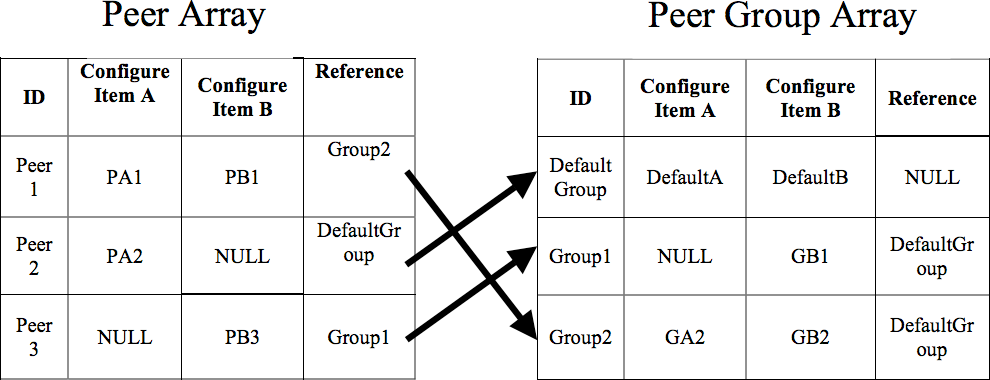
\includegraphics{figs/peerandpeergroup.pdf}}
\caption{An example of Peers and Peer Groups}
\label{fig:peerandpeergroup}
\end{figure}

From the above example, you can see the structures of peers and peer groups share the same set of configure items. In our design, peer structure and peer group structure share the same substructure "configuration" that includes all the configure items.  
Specifically peer structure consists of three parts:
\begin{itemize}
\item{\emph{Peer ID:}  It is the identifier of a peer, starting from 0. It is also the index of a peer in the array.} 

\item{\emph{Session ID:} It is  the identifier of a peering session that is associated with a peer, starting from 0. For the disabled peer, it is -1. Peering session will be discussed in the next subsection.}

\item{\emph{Configuration Substructure:} It contains all configure items needed in peer configuration.}  
\end{itemize}
And peer group structure also consists of three parts:
\begin{itemize}
\item{\emph{Peer Group ID:}  It is the identifier of a peer group, starting from 0. It is also the index of a peer group in the array.} 

\item{\emph{Peer Group Name:} It is the name of a peer group.}

\item{\emph{Configuration Substructure:} It is same as the configuration substructure in peer structure.}  
\end{itemize}
Configuration substructure includes all the configure items which are needed by peering session establishment, labeling module and periodic event handling module. Figure \ref{fig:configurationSub} shows the details of configuration substructure. All of these configure items except "routerRefreshAction" and "labelAction" are used to establish a peering session. "routerRefreshAction" is used by periodic event handling module and "labelAction" is used by labeling module.
\begin{figure*}
\centering
\scalebox{1}{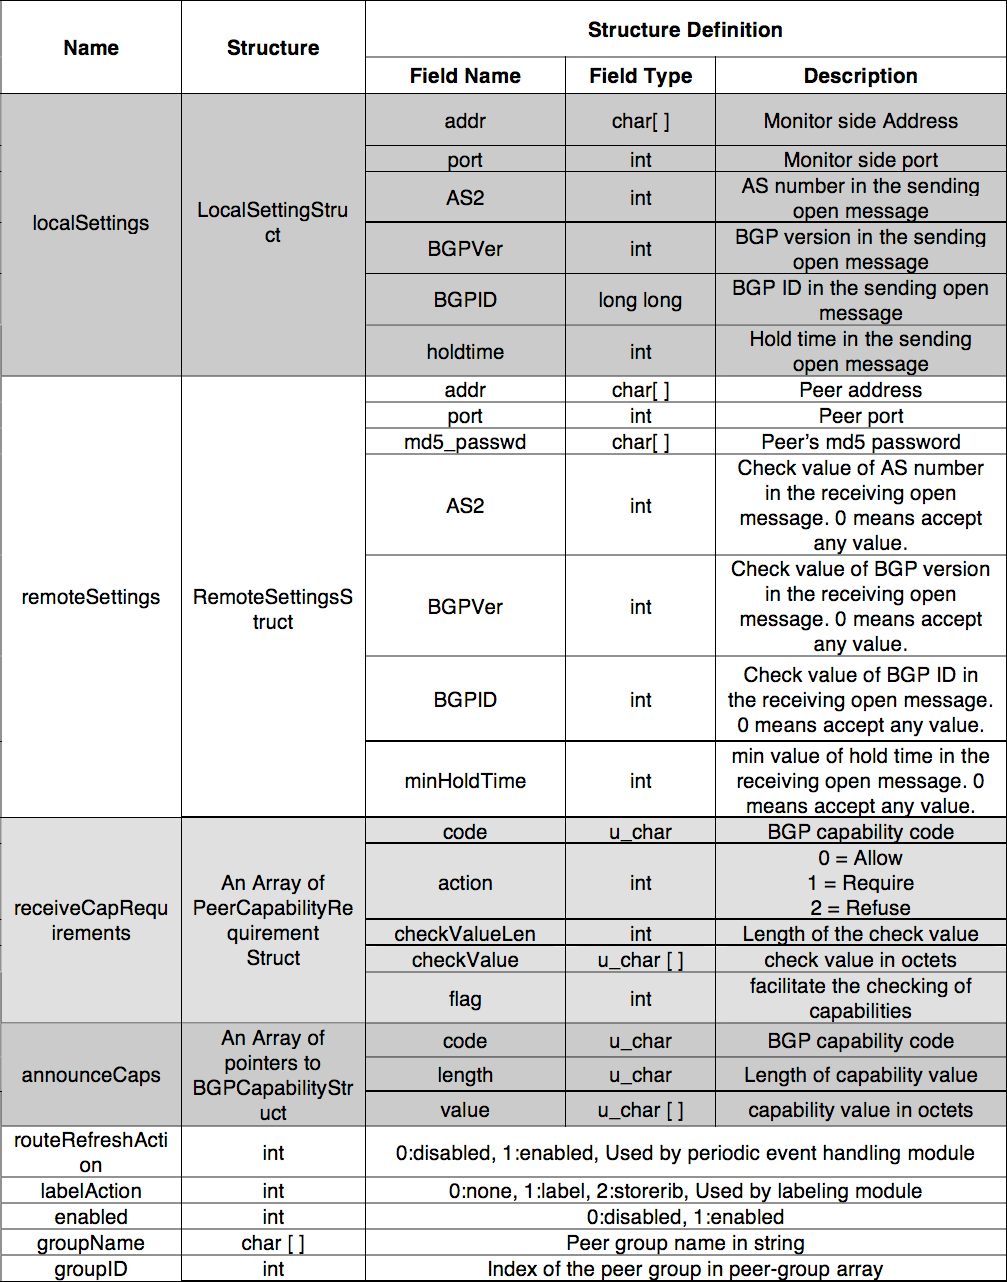
\includegraphics{figs/configurationSub.pdf}}
\caption{Configuration Substructure}
\label{fig:configurationSub}
\end{figure*}

Peering module also provides a bunch of functions to create, delete, read and write peers and peer groups.  Command line interface uses these functions to manipulate peer configuration. We have discussed the peer configuration so far. Next peering session will be discussed. 

\subsection{Peering  Session}
Peering module maintains an array that holds the data for all peering sessions and each element in this array is a "Session" structure. "Session" structure is not only used by peering module but also used by labeling module, periodic event handling module and XML module.
As we mentioned each enabled peer has its own thread and these threads create "Session" structures in the array and uses them to establish and maintain the peering sessions. In each peer's thread, a peering session gets established by using the latest configuration of that peer. When a peering session is established, all the configure items that are used to establish the session will be saved in the "Session" structure. After that, any changes in those configure items via command line interface will not take effect until the peering session resets. And the peering session could be reset in the following 2 cases.
\begin{itemize}
\item{Users reset the peering session explicitly by issuing a reset command via command line interface. This happens typically when users change some peer configuration via command line interface and want these changes to be applied immediately. } 
\item{Peering session resets by itself. For example, the underlying tcp connection failure could cause a peer session reset.  Or the peering session could be reset if the peer fails for some reason.   }  
\end{itemize}
No matter why the peering session is reset, the latest peer configuration will be used when it gets established again. 
An important design decision here is that a new "Session" structure with new session ID will be created and used by the thread every time a peering session is reset.  Note even the thread is using the new "Session" structure, the old one will still stay in the session array for a while until it is not needed. We will discuss the design philosophy behind this in the next subsection.
In the remaining part of this subsection, the detail of "Session" structure will be discussed at first and then an introduction of how to establish and maintain a peering session by using "Session" structure will be given.

\subsubsection{"Session" Structure}
\label{sec:peering:sessionstructure}
Most fields of a "Session" structure are related to the peering module and a few fields are related to other modules. The details are shown as follows:
\begin{itemize}

\item{\emph{sessionID:} is the identification of a peering session which starts from 0. It is also the index of a peering session in the array.}

\item{\emph{ConfigInUse substructure:} is same as the configuration substructure shown in Figure \ref{fig:configurationSub}.   It is basically a copy of peer configuration when peering session gets established. It will not be changed once the peering session gets established. This substructure is important if one wants to know what are the differences between the latest peer configuration and the configuration used to establish the peering session.}

\item{\emph{FSM substructure:} is a group of fields that are used to maintain the BGP Finite State Machine (FSM) such as state of FSM, socket and a couple of timers. Figure \ref{fig:FSMSub} shows the details of FSM substructure.}
\begin{figure*}
\centering
\scalebox{0.9}{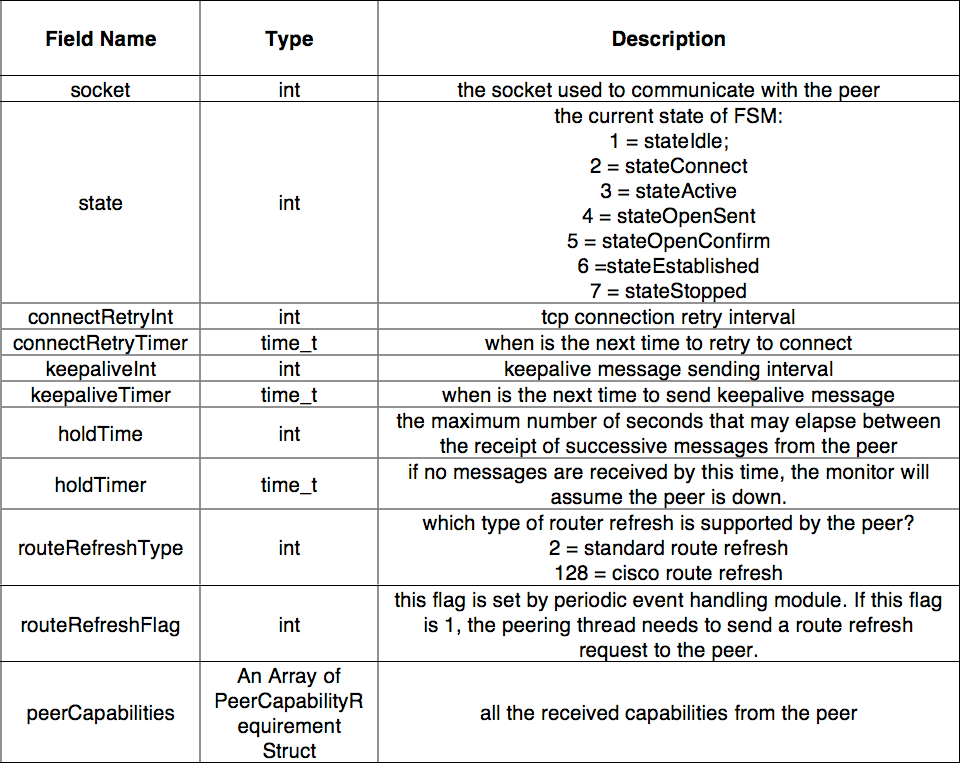
\includegraphics{figs/FSMSub.pdf}}
\caption{FSM Substructure}
\label{fig:FSMSub}
\end{figure*}

\item{\emph{Statistics substructure:} is a group of fields related to the peer's statistics such as the time of last session reset and the number of received updates. Figure \ref{fig:StatSub} shows the details of statistics substructure}
\begin{figure*}
\centering
\scalebox{0.9}{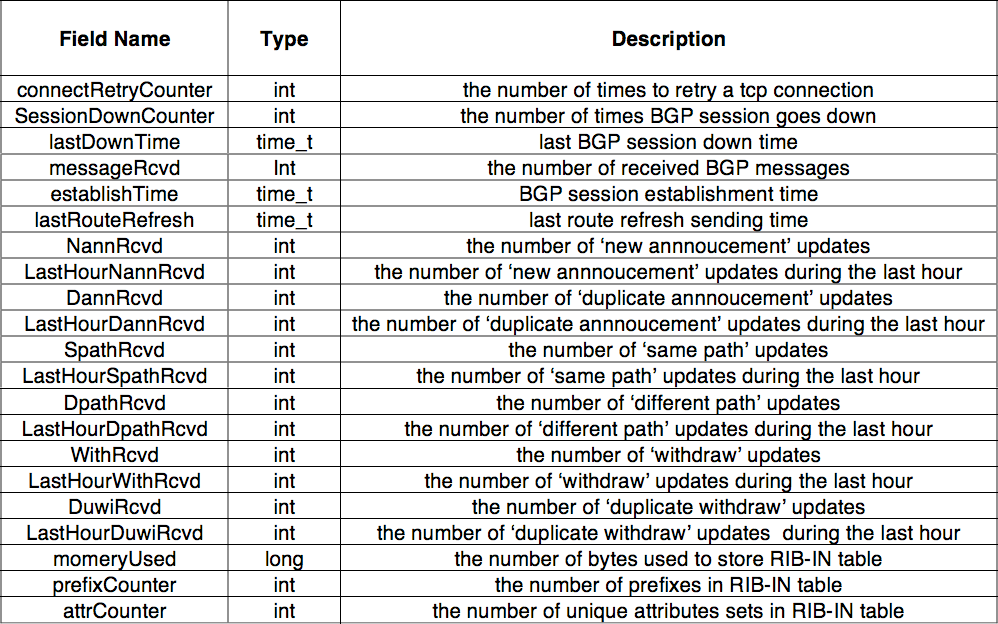
\includegraphics{figs/StatSub.pdf}}
\caption{Statistics Substructure}
\label{fig:StatSub}
\end{figure*}

\item{\emph{peerQueueWriter:} is used to write the messages exchanged between BGPmon and the peer into the queue. }

\item{\emph{sessionStringOutgoing:} is a XML string generated by peering module. It is used by XML module as the common XML header of all outgoing messages. It consists of 2 triples: Source triple and Destination triple.
Source triple contains monitor side address port and AS number.  Destination triple contains peer's address, port and AS number.   }

\item{\emph{sessionStringIncoming:} is similar to sessionStringOutgoing. It is a common XML header for all incoming messages. In this XML string, source triple contains peer address port and AS number.  Destination triple contains monitor side address, port and AS number. }

\item{\emph{PrefixTable Substructure and AttrTable Substructure:} are used to maintain a RIB table. They are initialized by peering module and populated by labeling module. The detail of them will be discussed in Section \ref{sec:labeling}. }

\item{\emph{reconnectFlag:} is used to reset a peering session and set by command line interface. This flag is typically set when a user wants the changes of peer configuration to be applied. }

\item{\emph{lastAction:} is a timestamp that indicates when the last action of a peering session is. It is used to check if a peering session is running correctly. }

\end{itemize}

\subsubsection{Establish and Maintain Peering Sessions}

To establish a BGP peering session, the first step in peer's thread is to create a socket and bind it to the monitor side address and a port specified in "localSettings" of the peer configuration( See Figure \ref{fig:configurationSub}). 
Secondly, the thread needs to initiate a tcp connection to the peer actively. Similarly, the peer's address and port are specified in "remoteSettings" of the peer configuration. Note in our design the thread always initiates the connection actively and simply drops all the incoming connection from the peer for the security purpose.

Once the tcp connection is established, the thread will exchange the BGP open message with the peer. As shown in  Figure \ref{fig:configurationSub}, all the parameters(BGP version, BGP ID, AS number and holdtime) needed to create a BGP open message can be found in "localSettings" of configuration substructure. Also all announcing capabilities included in the open message can be found in "announceCaps" of configuration substructure.
Then the thread sends the created open message via the established tcp connection and waits for the incoming open message from the peer. 

Upon receiving the open message, the thread will do the following two checks.
\begin{itemize}
\item{ Check the version, AS number, Identifier and holdtime in the received open message against the expected values specified in "remoteSetting" of configuration substructure( See Figure \ref{fig:configurationSub}). }
\item{ Check the capabilities in the received open message against the capability requirements specified in "receiveCapRequirements" of the configuration substructure(Figure \ref{fig:configurationSub}). For each capability $A$ in capability requirements, there are three possible actions:  }
\begin{itemize}
\item{ \emph{Allow:} nothing needs to be done.}
\item{ \emph{Require:} check if the received capabilities contain $A$ and the value of the received capability is same as the check value is configured. If no, check fails.}
\item{ \emph{Refuse:} check if the received capabilities contain $A$ and the value of the received capability is same as the check value is configured. If yes, check fails. }
\end{itemize}
\end{itemize}
If any of these checks fails, the thread will send a notification message to the peer and close the connection.
If all the checks pass, the thread will send a keepalive message to the peer and wait for another keepalive message from the peer. Once this keepalive message is received, the BGP peering session is successfully established. 

After the peering session gets established, the thread will periodically sent out keepalive messages if holdtime is not zero and route refresh requests if configured.

Each thread also writes two types of messages into the peer queue:
\begin{itemize}
\item{BGP Message: The BGP messages exchanged with the peer are written into the peer queue. Note no 'Update' messages will be sent from BGPmon. }
\item{FSM Message: The state changes of BGP finite state machine are written into the peer queue such as from 'Idle' to 'Connect', from 'OpenConfirm' to 'Established' and so on.}
\end{itemize}
These types of messages are converted into BGPmon internal format before being written into peer queue. After conversion, the session ID in the message indicates it belongs to which peering session.

In our design, periodic event handling module centralized manages and schedules the route refresh for all the peers. Instead of sending route refresh requests by itself, periodic event handling module notifies the peering module to send route refresh requests when needed. And the field 'routeRefreshFlag' in FMS substructure(Figure \ref{fig:FSMSub}) is used to notify peering module. 

\subsection{Design Philosophy}
In the design of peering module, one important issue is how to handle changes in a peer's configuration when the peer already has a existing peering session. Most of configuration changes will only take effect by resetting the existing peering session such as changes in monitor address, port or AS number. But it is not practical to reset a peering session every time such a change happens. Probably one might want to reset the peering session after a series of changes is done. So we decided to let the user make the decision about when to reset the peering session. User can reset the peering session by issuing a command via command line interface. 

As a result of letting user make the decision when to make configuration changes take effect, it is necessary to provide the user with the difference between the latest peer configuration and the configuration used to establish the existing peering session.
This explains why we need a "ConfigInUse" substructure in a "Session" structure. The "ConfigInUse" substructure is copied from peer configuration when peering session is established and will not be changed after that.
By comparing the "ConfigInUse" of a peering session and the latest peer configuration, the user will know all the changes of a peer configuration since its peering session was established. 

Another important design issue is that a new "Session" structure with new session ID will be created and used by the thread every time a peering session is reset. The reason is related to the BGPmon architecture and the format of BMF message.
As we discussed, modules of BGPmon are connected by queues and every message in peer queue and label queue has a session ID field. 
The session ID will be used as the key to retrieve the information needed to process the BMF messages by other modules such as labeling module and XML module.
For example, XML module needs the session ID to get the XML common header("sessionStringOutgoing" and "sessionStringOutgoing" in a "Session" Structure) in order to convert a BMF message to a XML string.
In BGPmon it is possible that some BMF messages associated with old peering session are buffered in the queue after a peering session gets reset . 
In this case if the peer's thread doesn't create a new "Session" structure and simply uses the same "Session" structure, XML module will wrongly convert the BMF messages associated with old peering session by using the XML common header of new peering session.
In order to avoid this,  the peer's thread needs to create a new "Session" structure and keep the old "Session" structure when a peering session is reset. After peering session reset, the peer's thread will use the new "Session" structure and tag the new BMF messages with new session ID.
The old "Session" structure will finally be deleted after all the BMF message associated with the old peering session are processed. 
%\subsection{Data Structure}
%The single key data structure of peering module is called session. Each peering thread is attached with a session structure. The session structure consists of five parts:
%\begin{itemize}

%\item{\emph{sessionID:} is 16 bit session identification. It is started from 1 and each peering thread is associated with a unique SessionID.}

%\item{\emph{Configuration substructure:} includes all the configurations of a peer which are needed to establish the BGP session such as peer's address and AS number. It is created by configuration module. The Configuration Module will write this section and the Peering Module will only read it.}

%\item{\emph{FSM substructure:} is a set of fields which are related the BGP Finite State Machine (FSM) used to maintain the BGP session.   The Peer Module will write and read this section.   Other modules may read this section to learn the status of a peer.}

%\item{\emph{Statistics substructure:} is a group of fields related to the peer's statistics such as the time of last session reset and the number of received updates.    The Peer Module will write and read this section.   Other modules may read this section to learn statistics about this peer.}

%\item{\emph{peerQueueWriter:} It is used to write the messages received from peers to the peer queue. }

%Figure \ref{fig:sessionStruct} shows the session structure.
%%\begin{figure*}
%%\centering
%%\caption{BGPmon Internal Message Types}
%%\label{tab:sessionStruct}
%%\end{figure*}

%%\begin{figure}[!htb]
%\begin{figure}[!htb]
%\scalebox{0.56}{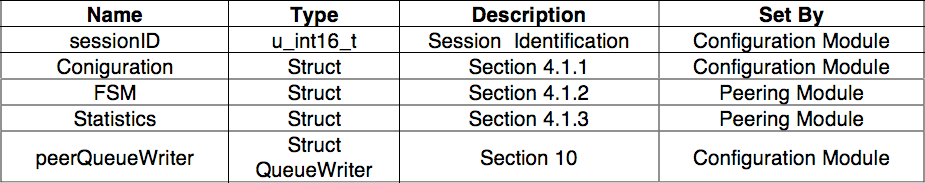
\includegraphics{figs/sessionStruct.pdf}}
%\caption{Session Structure}
%\label{fig:sessionStruct}
%\end{figure}

%%\begin{figure*}
%%\centering
%%\begin{tabular}{| l | l | l |}
%%\hline
%%sessionID & $u_int16_t $ & Session  Identification & Configuration Module\\
%%\hline
%%configuration & struct & Section 4.1.1 & Configuration Module\\
%%\hline
%%FSM & struct & Section 4.1.2 & Peering Module\\
%%\hline
%%statistics & struct & Section 4.1.3 & Peering Module\\
%%\hline
%%\end{tabular}
%%\caption{Session Structure}
%%\label{tab:sessionStruc}
%%\end{figure*}
%\end{itemize}

%\subsubsection{Configuration  SubStructure}
%Configuration SubStructure consists of six parts. 
%\begin{itemize}
%\item{\emph{BGP Open Message:}  It is the BGP open message sent to the peer in order to establish the BGP session.} 

%\item{\emph{Monitor Settings:} It contains a protocol independent address structure which is used to open the socket and a hold time used to negotiate the final hold time with the peer. }

%\item{\emph{Router Settings:} First it contains a protocol independent address structure and optional MD5 password which are used to connect to the peer. Secondly it contains the expected AS number, BGP version, BGP Identifier and minimal hold time. The received open message from the peer is checked against these expected values. }

%\item{\emph{Capability Requirements:} It contains a array of capability requirements based on the configuration. The received capabilities from the peer are checked against these capability requirements. }

%\item{\emph{Desired Configuration:} It is used to signal the peering module the changes in configuration. It will be incremented by one every time the configuration is changed by configuration module. }

%\item{\emph{Enabled:} It is used to signal the current configured peer status(pause, normal or close). It is set by configuration module.   }

%\end{itemize}
%Figure \ref{fig:configurationSub} shows the details of configuration substructure. 
%\begin{figure*}
%\centering
%\scalebox{1}{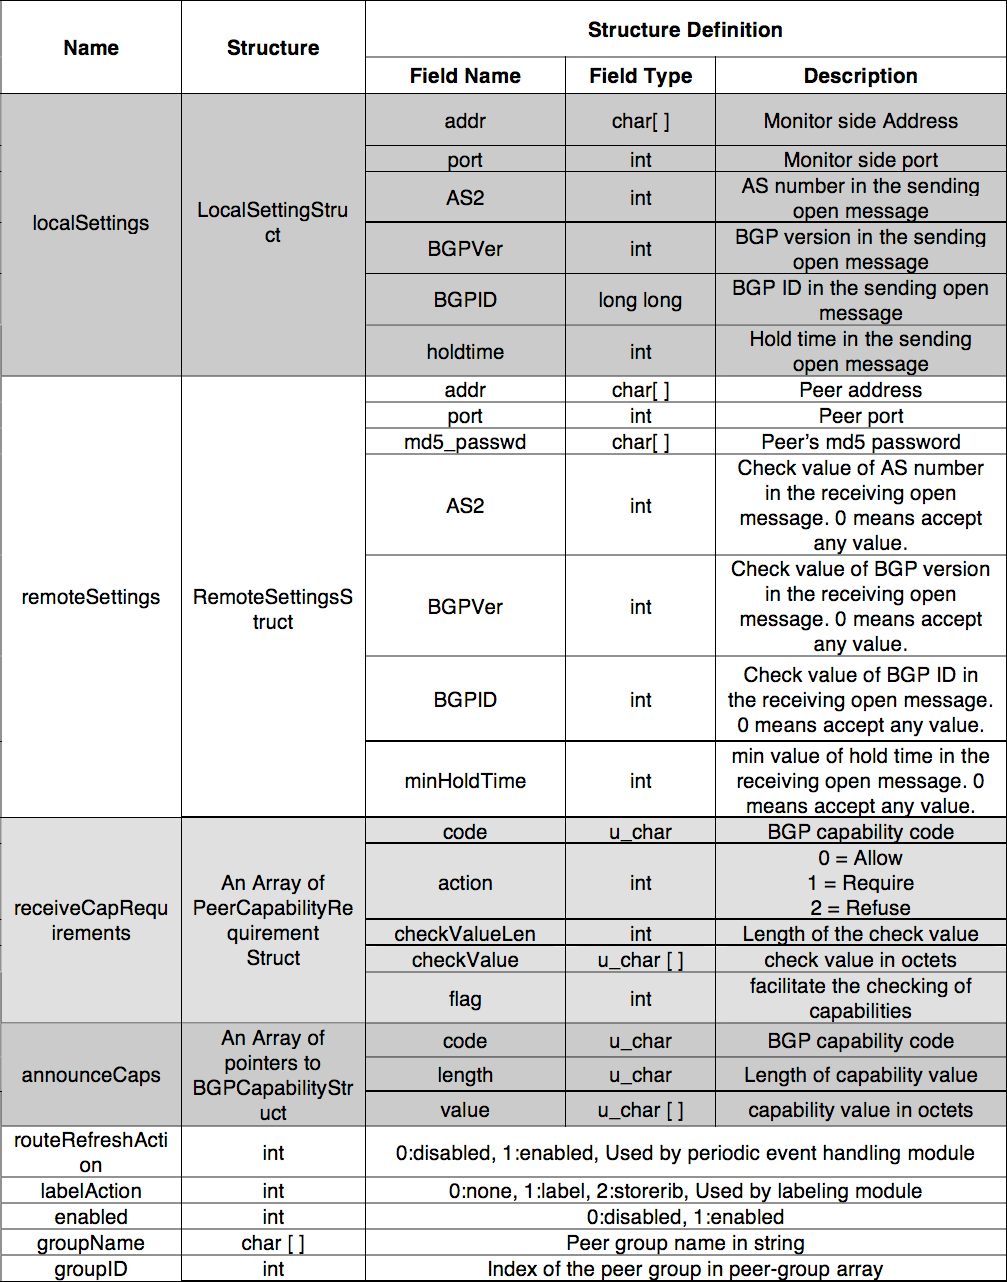
\includegraphics{figs/configurationSub.pdf}}
%\caption{Configuration Substructure}
%\label{fig:configurationSub}
%\end{figure*}

%\subsubsection{FSM SubStructure}
%FSM substructure contains all the information needed to maintain a BGP session.  It consists of a socket, the current state of FSM, and several timers.
%Figure \ref{fig:FSMSub} shows the details of FSM substructure.
%\begin{figure*}
%\centering
%\scalebox{1}{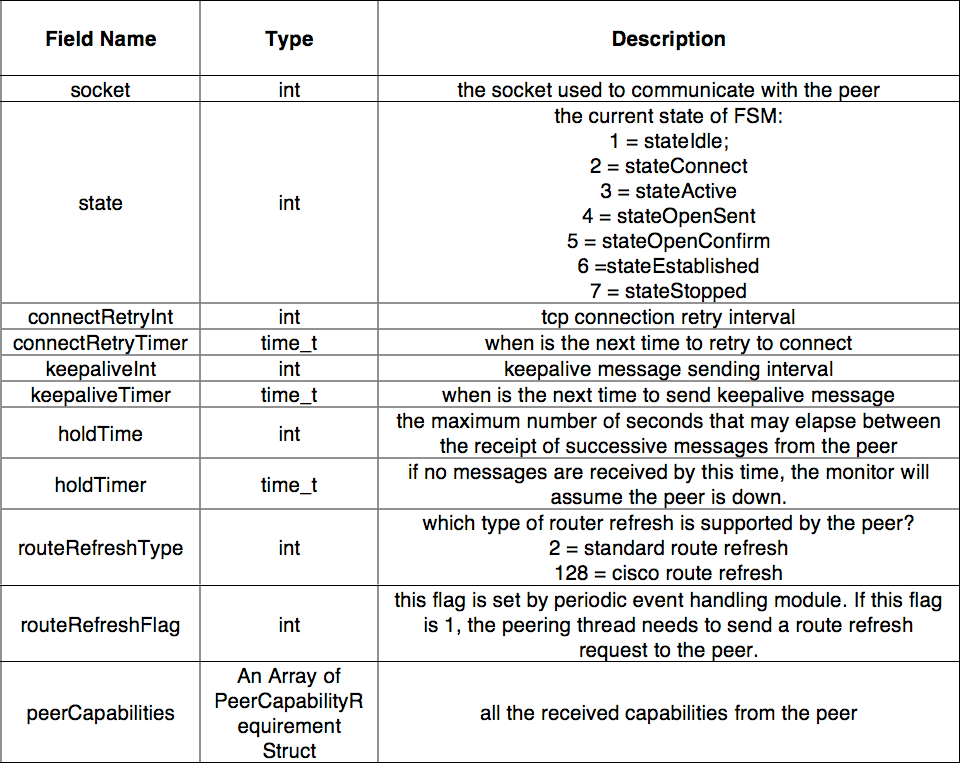
\includegraphics{figs/FSMSub.pdf}}
%\caption{FSM Substructure}
%\label{fig:FSMSub}
%\end{figure*}

%\subsubsection{Statistics SubStructure}
%Statistics substructure contains the peer's statistical information. 
%Figure \ref{fig:StatSub} shows the details of statistics substructure.
%\begin{figure*}
%\centering
%\scalebox{1}{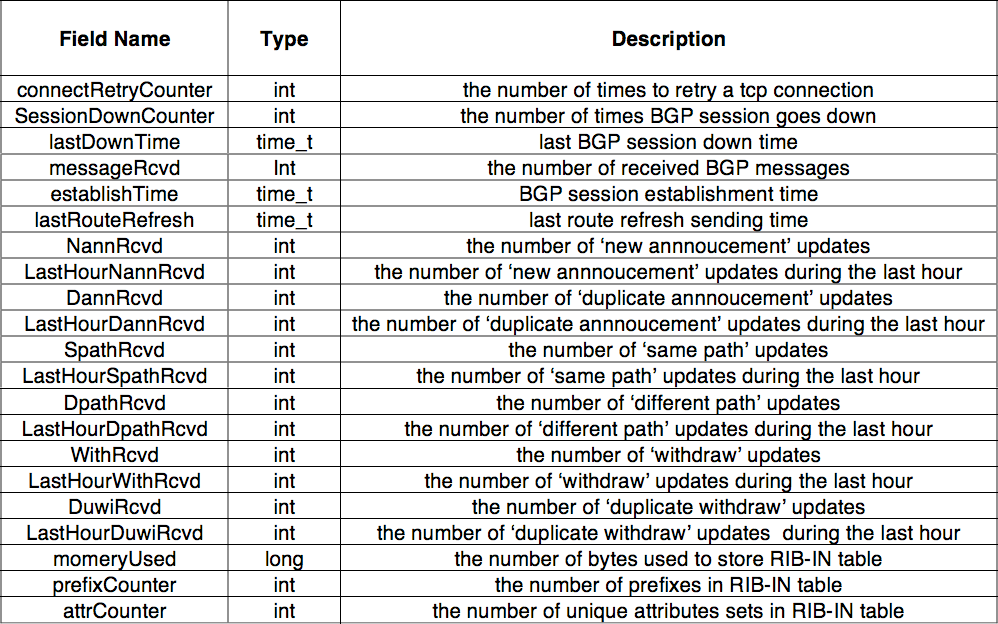
\includegraphics{figs/StatSub.pdf}}
%\caption{Statistics Substructure}
%\label{fig:StatSub}
%\end{figure*}

%\subsection{Opening and Maintaining Peering Sessions}

%% opening the socket....     note config has set address.    do not care if this is IPv4 or Ipv6 or other.
%The first step of peering thread is to create a socket and bind it to a interface and a port if configured. According to Figure \ref{fig:configurationSub}, configuration module has created monitor's protocol independent address structure.  This structure contains all the information needed to create sockets and bind sockets such as address family, socket type, address and port. So the peering thread can simply create and bind a socket with this protocol independent address structure without knowing its content such as its address family(IPv4 or IPv6) and the port number. 

%Secondly, the peering thread needs to establish the tcp connection with the router actively. Similarly, configuration module has created router's protocol independent address structure. The peering thread can establish the tcp connection by using the created socket and the router's protocol independent address structure.
%Note in our design the peering thread always initiates the connection actively and simply drops all the incoming connection from the router for the security purpose.

%Once the tcp connection is established, the peering thread will exchange the BGP open message with the peer. As we mentioned before, configuration module has created the open message and included all desired capabilities(Figure \ref{fig:configurationSub}). The peering thread just sends the created open message via the established tcp connection and waits for the incoming open message from the peer. Upon receiving the open message, the peering thread will do the following two checks.
%\begin{itemize}
%\item{ Check the version, AS number, Identifier and holdtime in the received open message against the expected values of them in the configuration substructure(Figure \ref{fig:configurationSub}). }
%\item{ Check the capabilities in the received open message against the capability requirements in the configuration substructure(Figure \ref{fig:configurationSub}). For each capability $A$ in capability requirements, there are three possible actions:  }
%\begin{itemize}
%\item{ \emph{Allow:} nothing needs to be checked.}
%\item{ \emph{Require:} check if the received capabilities contain $A$ and the value of the received capability is same as the check value is configured. If no, check fails.}
%\item{ \emph{Refuse:} check if the received capabilities contain $A$ and the value of the received capability is same as the check value is configured. If yes, check fails. }
%\end{itemize}
%\end{itemize}
%If any of these checks fails, the peering thread will send a notification message to the peer and close the connection.
%If all the checks pass, the peering thread will send a keepalive message to the peer and wait for another keepalive message from the peer. Once this keepalive message is received, the BGP session is successfully established. 

%After the BGP session gets established, the peering thread will periodically sent out keepalive messages if holdtime is not zero and route refresh requests if the peer supports it.
%   

%% sending the open message....   note config has set open message and included all desired capabilities.
%% checking the capabilities....     how does it do this?   what notifies are sent?
%%Figure \ref{fig:capstruct} show the capabilities structure used by the peering module.
%%maintaining the connection....    sending and receiving keepalives.     what if hold time is zero?   what notifies might be sent?

%Each peering thread also writes two types of messages into the peer queue:
%\begin{itemize}
%\item{BGP Message: The BGP messages sent or received by the peering threads are written into the peer queue. Note no 'Update' messages are sent from the peering thread to peering router. }
%\item{FSM Message: The state changes of BGP finite state machine made by the peering thread are written into the peer queue such as from 'Idle' to 'Connect', from 'OpenConfirm' to 'Established' and so on.}
%%\item{Peer Status Message: The states of the peer are written into the queue. The states of peer can be very simple such as the peer's address and AS number.  It also can be complex such as the BGP capabilities received from the peer. }
%\end{itemize}
%These types of messages are converted into BGPmon internal format by peering threads before being written into peer queue.

%%\subsection{Maintaining Statistics}
%% what do we maintain?     last action time,  bytes recvd, bytes sent, ??

%\subsection{Route Refresh}
%% how do we request this?
%Periodic event handling module centralized manages and schedules the route refresh for all the peers. Instead of sending route refresh requests by itself, periodic event handling module notifies the peering threads to send route refresh requests when needed. And a field 'routeRefreshFlag' in FMS substructure(Figure \ref{fig:FSMSub}) is set to notify peering thread by periodic event handling module.  Each peering thread reads this flag field after every step in FSM and it needs to send the router refresh request to the peer if this flag is set to 1. 

%% what do we do if we receive one?

%%\subsection{Closing Peering Sessions}
%%Configuration module may need to close a peering session in some cases. Similar to the route refresh case, configuration module notifies the peering thread to close a peering session by setting a field 'close flag' in FMS substructure(Figure \ref{fig:FSMSub}). Each peering thread checks this flag field after every step in FSM. If it is set to 1, the peering thread needs to send a notification message to the peer before closing the tcp connection.

%\subsection{Dynamic Configuration Change}
%The last design issue in this section is how peering thread detects the dynamic configuration changes. In our approach there are two sequence numbers associated with the configuration substructure and FSM substructure. The one in FSM substructure is called 'configurationInUse' which indicates the configuration using by peering thread. Another in configuration substructure is called 'desiredConfiguration' which indicates the latest configuration set by configuration module. 'desiredConfiguration' will be increased by configuration module when the configuration changes. Besides this two sequence numbers, there is another flag in configuration substructure called 'enable'. This flag which is et by configuration module indicates which action should be done by peering thread after a configuration change. 

%Right after every step in FSM, the peering thread will do the following checks:
%\begin{itemize}
%\item{ If 'configurationInUse' is smaller than 'desiredConfiguration', sends notification message,  clean the corresponding RIB-IN table and close the TCP connection if BGP session is established.}
%	\begin{itemize}
%	\item{If 'enable' is set to 0, pause the FSM and don't try to open a new session.}
%	\item{If 'enable' is set to 1, open a new BGP session.}
%	\item{If 'enable' is set to 2, close the thread and set the state of FSM to 7(stateStopped).}
%	\end{itemize}
%\item{ Otherwise, do nothing.}
%\end{itemize}

%%if $configurationInUse $ is smaller than $configurationInUse $. If yes, peering thread needs to restart the BGP session and also set $PeeringConf$  as same as $CurrentConf$.

%
%Obviously there is a delay between configuration module changes the configuration and peering thread uses the changed configuration. The delay depends on how long a step of FSM takes. In a extreme case, if a peering doesn't support keepalive messages, the changed configuration will not take effect until the next incoming BGP update. Such a long delay is not acceptable. In order to solve this problem, we can introduce a dedicated timer to check the configuration periodically. 

%Basically all the parts except configuration substructure in session structure are created by configuration module and then maintained by peering module. But for the configuration substructure,  it still needs to be maintained by configuration module after creation in order to support dynamically configuration. 
%More specifically, there are two steps to support dynamically configuration.
%\begin{itemize}
%\item{Configuration module changes the configuration substructure inside a session structure after the user changes the peer's configuration.}
%\item{Peering module needs to detect the changes quickly and do the corresponding actions. For example, if the peer's address changes the session must be reestablished. }
%\end{itemize}
\section{MRT Module Test Unit}
\label{sec:mrt}


%Before start using \emph{MRT} testbed, its important for the user of framework to get the right understanding of MRT unit design and its role in BGPmon Test Framework.  
The \emph{MRT} unit allows one to inject MRT messages into the BGP Test Framework.  MRT messages do not come directly from a peer router. Instead they are collected by a third party and then reported to BGPmon.    An MRT message consists of a header followed by a BGP message. The header specifies the time when the message was collected and the peer that sent the message. 

% MRT messages are collected   by third parties from indirectly connected peers through third parties. 
 
The MRT unit supports two models for injecting MRT data. In the \emph{end-user} model an external user supplies the MRT data as set of files.   For example, a user may create MRT files that include BGP messages from one of her peer routers.  In the \emph{collector}
model, the tester provides a name of  RouteViews collector, a start time, and an end time.  For example, the tester may specify \emph{route-views2.oregon-ix.net}, starting from September 1st at 9:00 am, ending on September 12th at 3:00 pm. 
  
 
%  takes the fact that there are exist routing collectors that installed in Internet exchange points and collect routing data from many peers. For instance, Oregon RouteViews collectors has large number of IPv4 and IPv6 peers around the globe.   \emph{MRT} unit need to support both models no matter how fast or how often end-users or routing collectors  provide routing data to BGPmon application.  For instance, RouteViews project include more than 100 BGP peers around the world. Those peers create a very large set of updates that need to processes by BGPmon application fast and correctly. In the other hand, end-user may send small MRT file with just few BGP updates. Any MRT messages can not be dropped or ignored by BGPmon application.  

Unlike live data,  MRT files  have been collected already and each MRT message includes a time stamp. The testing  unit plays back the MRT messages, preserving the timing between messages.  For example, if the first BGP message originated at \emph{1:20:00 am} and second BGP message at \emph{1:25:00 am},  the MRT testing unit will send the first BGP message, sleep for \emph{5 minutes} and only then send the second BGP message. 

%Using \emph{timeframing} helps to create a sequence of BGP messages ordered by the time they were created at the third party.  

%Furthermore, the user of framework need to be familiar with \emph{timeframing} in MRT unit. Because MRT unit provide routing data from third parties, BGP message  timestamping plays important role in reconstructing precise routing picture on BGPmon instance. In particular, MRT format header contains  date and time  when BGP message was received at the third party. In order to replicate the right order of BGP messages, MRT unit uses the notion of \emph{timeframing}. \emph{Timeframing} is a mechanism to send BGP messages using the difference of  timestamps in subsequent BGP messages. For example, if first BGP messages originated at \emph{1:20:00 am} and second BGP messages at \emph{1:25:00 am},  MRT unit will send first BGP message and sleep for \emph{5 minutes} and only then send second BGP message. Using \emph{timeframing} helps to create a sequence of BGP messages ordered by the time they were created at the third party.  

%The  \emph{MRT}  unit is designed to achieve following goals:

%\begin{itemize}
%\item{Test BGPmon instance to receive MRT data stream.  }
%\item{Keep MRT sessions: this verifies that BGPmon is able to keep MRT %sessions alive using data from MRT stream.}
%\item{BGPmon receives routes: this verifies that BGPmon is able to extract %routes from MRT stream.}

%\item{Test BGPmon instance to scale out through chaining multiple BGPmons.   This verifies BGPmon's Chain Module functionality to create a TCP connection to another BGPmon.}
%\item{Receive XML stream: this verifies that BGPmon is able to receive XML messages from connected chain instance.}
%\end{itemize}

%\subsection{IPv4 MRT Unit Overview}

\begin{figure}
\centering
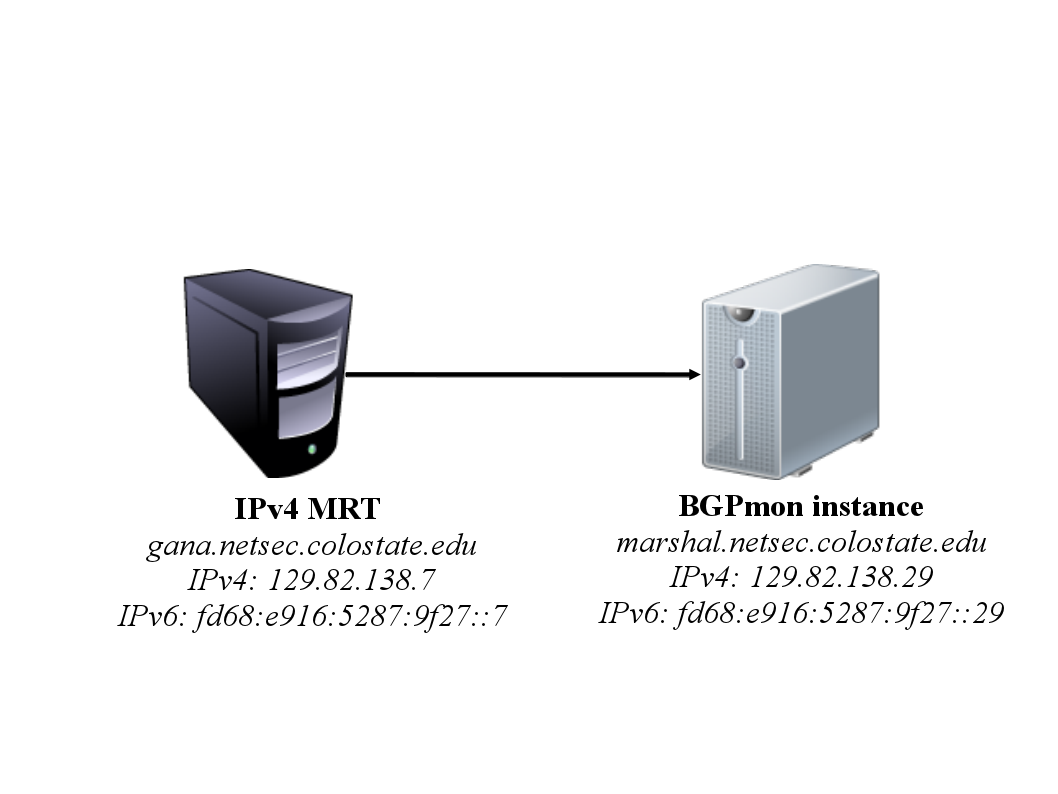
\includegraphics[scale=0.30]{figs/ipv4-mrt.png}
\caption{An overview of IPv4 MRT Unit.}
\label{mrtfig}
\end{figure}

Figure \ref{mrtfig} shows the test unit design: it includes an MRT sender and BGPmon receiver.  The  MRT sender is installed on \emph{gana.netsec.colostate.edu} with an IPv4 address of  \emph{129.82.138.7} and an IPv6 address of \emph{fd68:e916:5287:9f27::7}. The BGPmon receiver is  installed on \emph{marshal.netsec.colostate.edu} with an IPv4 address of  \emph{129.82.138.29} and IPv6 address of \emph{fd68:e916:5287:9f27::29}. 

\subsection{Configuring BGPmon to Receive MRT}
\label{sec:mrtbgpmoness}


To configure BGPmon to receive MRT data: 

\begin{enumerate}
  \item{Login to \emph{marshal.netsec.colostate.edu}}
  \item{Make sure that the BGPmon process is up and running. If not, see Section \ref{sec:essentials}.}
  \item{Telnet to \emph{localhost} port \emph{50000} to access the Command Line Interface.}
  \item{In \emph{configuration mode}, launch the \emph{mrt-listener}:}
\begin{verbatim}
marshal$ enable
marshal# configure
marshal(config)# mrt-listener enable
marshal(config)# end
\end{verbatim}      
\end{enumerate}

This command instructs BGPmon to listen for  TCP connections on \emph{marshal.netsec.colostate.edu}.   \emph{Mrt-listener } will use IPv4 address of  \emph{129.82.138.29}, port \emph{7777} and IPv6 address of \emph{fd68:e916:5287:9f27::29}, port \emph{7777} for incoming connections. 

The user of framework may configure \emph{mrt-listener} to listen for TCP connections on IPv4 address only. Run following command in \emph{configuration mode}:
\begin{verbatim}
    marshal$ enable
    marshal# configure
    marshal(config)# mrt-listener address 129.82.138.29
    marshal(config)# mrt-listener enable
    marshal(config)# end
\end{verbatim}

To configure \emph{mrt-listener} to listen for TCP connections on IPv6 address only, run:
\begin{verbatim}
    marshal$ enable
    marshal# configure
    marshal(config)# mrt-listener address fd68:e916:5287:9f27::29
    marshal(config)# mrt-listener enable
    marshal(config)# end
\end{verbatim}



%NEEDS WORK: What IP addresses are used?


%NEEDS WORK: How do we know if MRT listener is running? 
The tester of the framework can check status of    \emph{mrt-listener}. Run following command in Command Line Interface:
\begin{verbatim}
    marshal>show mrt-listener status
\end{verbatim}

This command shows \emph{mrt-listener} status. Successful configuration of  \emph{mrt-listener} will show \emph{enabled} status. Failed configuration of \emph{mrt-listener} will show \emph{disabled} status.

The tester of the framework may check the network IP addresses configured in \emph{mrt-listener}: 
\begin{verbatim}
    marshal>show mrt-listener address
\end{verbatim}

To disable the \emph{mrt-listener}  in BGPmon, run:
\begin{verbatim}
    marshal$ enable
    marshal# configure
    marshal(config)# mrt-listener disable
    marshal(config)# end
\end{verbatim}

This command instructs \emph{mrt-listener} to close TCP connections and change internal status to \emph{disabled}.



\subsection{Sending MRT Messages}

The MRT unit supports two models for injecting MRT data. In the \emph{end-user} model an external user supplies the MRT data as set of files.   In the \emph{collector} model, the tester provides a name of  RouteViews collector, a start time and an end time. 

\subsubsection{The End-user Model}

This model assumes the tester has one or more MRT files.   The tester may use his own MRT file or sample MRT file.   A sample MRT file (\emph{updates.20110916.1715})  is available on \emph{gana.netsec.colostate.edu} in the directory \emph{$\sim$bgpmoner/Development/bgpmon-dev/test/mrt\_harness/etc}.  This file was generated by \emph{route-views.oregon-ix.net} on \emph{September 16th 2011, 17:15 pm}. 

The tester of the framework need to be familiar with MRT unit directories on \emph{gana.netsec.colostate.edu}. \emph{$\sim$bgpmoner/Development/bgpmon-dev/test/mrt\_harness/etc} is directory that designed to store long-lasting files. Directory includes files that are the part of the MRT unit.  \emph{$\sim$bgpmoner/Development/bgpmon-dev/test/mrt\_harness/data} is temporary working directory. \emph{$\sim$bgpmoner/Development/bgpmon-dev/test/mrt\_harness/data}  is created to   store an optional data including  the testing MRT files. The user of the framework is allowed to store temporary files in    \emph{$\sim$bgpmoner/Development/bgpmon-dev/test/mrt\_harness/data} directory.

 
%If user chooses to use sample MRT file, he need to extract it from \emph{$\sim$bgpmoner/Development/bgpmon-dev/test/mrt\_harness/etc} and copy to  \emph{$\sim$bgpmoner/Development/bgpmon-dev/test/mrt\_harness/data}

%\begin{verbatim}
%$ cd ~bgpmoner/Development/bgpmon-dev/test/mrt\_harness/etc
%$ bunzip2  updates.20110916.1715.bz2
%$ cp updates.20110916.1715 
%               ~bgpmoner/Development/bgpmon-dev/test/mrt\_harness/data
%\end{verbatim}

%If user chooses to use his own MRT file, he need to copy it to \emph{ %$\sim$bgpmoner/Development/bgpmon-dev/test/mrt\_harness/data}.

To start MRT unit test, run following: 

\begin{enumerate}
  \item{Download the MRT files into \emph{$\sim$bgpmoner/Development/bgpmon-dev/test/mrt\_harness/data} folder or copy sample MRT file from \emph{$\sim$bgpmoner/Development/bgpmon-dev/test/mrt\_harness/etc} directory. }
  
  \item{Login to \emph{gana.netsec.colostate.edu}.}
  \begin{enumerate}
  \item{To send MRT data from \emph{filename},  run:}
\begin{verbatim}
$ mrtfeeder -f filename -d marshal.netsec.colostate.edu
\end{verbatim}
   where:
  \begin{itemize}
  \item{\emph{filename} is MRT file name in \emph{$\sim$bgpmoner/Development/bgpmon-dev/test/mrt\_harness/data}. See Section \ref{sec:mrtfeederdesign} for the details about supported \emph{filename} extensions. } 
  \item{\emph{marshal.netsec.colostate.edu} is hostname of  BGPmon receiver. MRT feeder converts
\emph{marshal.netsec.colostate.edu} hostname to an IPv4 and an IPv6 socket address structures. MRT feeder connects to BGPmon receiver using one of socket address structures. }
  \end{itemize}  
  \item{The tester of the framework may test MRT unit over IPv4 connection. Use the IPv4 address of BGPmon receiver to run MRT feeder:   }
\begin{verbatim}
$ mrtfeeder -f filename -d 129.82.138.29
\end{verbatim} 
  \item{The tester of the framework may test MRT unit over IPv6 connection. Use the IPv6 address of BGPmon receiver to run MRT feeder:}
\begin{verbatim}
$ mrtfeeder -f filename -d fd68:e916:5287:9f27::29
\end{verbatim}    
           
  \end{enumerate}
\item{To see the results, see Section \ref{sec:mrtreport}.}
\end{enumerate} 

The MRT feeder send MRT file with MRT messages  to BGPmon receiver. As long as TCP connection is alive between MRT feeder and BGPmon receiver,  BGPmon receiver  keeps track of MRT peers and received routing data.  Once the MRT feeder reaches the last MRT message in MRT file, it will close TCP connection to BGPmon.  \emph{Mrt-listener}  will be triggered to destroy all MRT sessions and processed routes. To avoid this  situation and help the tester in debugging, the MRT feeder has an option that keeps TCP connection alive. The tester of the framework can run the MRT feeder with following option:  
  
\begin{verbatim}
        $ mrtfeeder -q -f filename -d marshal.netsec.colostate.edu
\end{verbatim}
where
\begin{itemize}
\item{\emph{-q} instructs MRT feeder to keep TCP connection alive after the last MRT message is sent to BGPmon. } 
\end{itemize}

In order to stop running MRT feeder, the tester of the framework need to type following command and  press \emph{RETURN} key on a keyboard. 
\begin{verbatim}
        exit
\end{verbatim}

This command will terminate MRT unit work. 



\subsubsection{The Collector Model}


In the collector model, the tester specifies the RouteViews collector, start time and end time.  The MRT unit injects the MRT messages from a specified RouteViews collector using adjusted time frame.
%The RouteViews collector collects the MRT messages from a directly connected peers.   
%The MRT unit is designed to send stream of consequent MRT files to BGPmon receiver.  
%The MRT unit uses MRT files from the RouteViews collector and sends MRT data directly to BGPmon application. 

The RouteViews collectors provide two types of MRT files: an MRT table file and an MRT update file.  The table MRT file is the snapshot of the MRT table messages. 
%The RouteView collector generate the MRT table file every two hours.  
The update MRT file is a  set of MRT update messages. 
%The RouteViews collectors generate the  MRT update file every 15 minutes.  
The tester of the the framework provide the time frame when the MRT unit starts sending MRT snapshot and MRT update files.  The MRT unit approximate the start time to fetch the most recent   MRT snapshot file and MRT update files.  The MRT unit sends  MRT update files in a sequence based on the specified start time and end time.   

%  The MRT unit stars sending  the MRT messages that corresponds to specified start time and it stops sending MRT messages at the specified end time.
 

% that corresponds to  the time when they originated start time and end time. 


%The RouteViews collector archiving MRT messages from directly connected peers.  The MRT unit uses archived MRT files to send an MRT data to the BGPmon receiver.   The MRT unit uses two types of MRT messages: a table MRT messages and an update MRT messages.  MRT unit provide both a table and an update MRT messages to BGPmon receiver. 

To start MRT unit test, run following: 

\begin{enumerate}
  \item{Login to \emph{gana.netsec.colostate.edu}.}
  \item{Run \emph{mrtfetcher} application with following options: }
\begin{verbatim}
$ mrtfetcher -c collector -s starttime -e endtime 
   -d marshal.netsec.colostate.edu
\end{verbatim}
  where:  
  \begin{itemize}
  \item{\emph{collector} can be  \emph{route-views.oregon-ix.net}, \emph{route-views2.routeviews.org} or other collectors. The list of existing collectors is available at \url{http://www.routeviews.org/} website.}
  \item{\emph{starttime} is a unix timestamp that specifies the start time.}
  \item{\emph{endtime} is a unix timestamp that specifies the end time.}
  \item{\emph{marshal.netsec.colostate.edu} is hostname of  BGPmon receiver. MRT feeder converts
\emph{marshal.netsec.colostate.edu} hostname to an IPv4 and an IPv6 socket address structures. MRT feeder connects to BGPmon receiver using one of socket address structures. }
  \end{itemize}
  \emph{Mrtfetcher}  will send MRT files from the collector starting at time \emph{starttime} and ending at \emph{endtime}. Section \ref{sec:mrtfetcherdesign} describes the design of \emph{mrtfetcher} application.
  \item{The tester of the framework may test MRT unit over IPv4 connection. Use the IPv4 address of BGPmon receiver::   }
\begin{verbatim}
$ mrtfetcher -c collector -s starttime -e endtime 
   -d 129.82.138.29
\end{verbatim} 
  \item{The tester of the framework may test MRT unit over IPv6 connection. Use the IPv6 address of BGPmon receiver:}
\begin{verbatim}
$ mrtfetcher -c collector -s starttime -e endtime 
   -d fd68:e916:5287:9f27::29
\end{verbatim}    
  
 \item{The tester of the framework may configure MRT fetcher to skip sending MRT table messages and send MRT update messages only:}
 \begin{verbatim}
$ mrtfetcher -u -c collector -s starttime -e endtime 
   -d marshal.netsec.colostate.edu
\end{verbatim}
where
\begin{itemize}
\item{\emph{-u} flag instructs MRT fetcher to send the MRT update messages to BGPmon.}
\end{itemize}
  
  
%  NEEDS WORK: MRT fetcher sends table first and update next. 

\item{To see the results, see Section \ref{sec:mrtreport}.}
\end{enumerate} 

BGPmon receiver receives MRT data and keeps track of MRT sessions with routing data.   
%As long as TCP connection is alive to MRT feeder,  BGPmon receiver  keeps track of MRT peers and routes.  
Once the MRT fetcher reaches the last MRT message in MRT file, the MRT fetcher will close TCP connection to BGPmon.  \emph{Mrt-listener}  will be triggered to destroy all MRT sessions and processed routes. To avoid this  situation and help the tester in debugging, the MRT fetcher has an option that keeps TCP connection alive. The tester of the framework can run the MRT fetcher with following option:  


%The MRT fetcher sends a sequence of MRT messages to BGPmon receiver. Once the MRT fetcher sent the last MRT message, it closes TCP connection to BGPmon receiver. BGPmon receiver  destroys the MRT session and removes all  received BGP messages.  The tester of the framework may find this situation is difficult to debug.  To aid in debugging,  MRT fetcher application has an option that keeps TCP session alive.    The tester of the framework can run the MRT fetcher with following option:  
\begin{verbatim}
        $ mrtfetcher -q -c collector -s starttime -e endtime 
             -d marshal.netsec.colostate.edu
\end{verbatim}
where
\begin{itemize}
\item{\emph{-q} instructs MRT fetcher to keep TCP connection alive after the last MRT message is sent to BGPmon. } 
\end{itemize}

In order to stop running MRT fetcher, the tester of the framework need to type following command and  press \emph{RETURN} key on the keyboard. 
\begin{verbatim}
        exit
\end{verbatim}

This command will terminate MRT fetch unit. 


\subsection{Result Reporting}
\label{sec:mrtreport}

The MRT unit provides a set of commands for debugging the problems in BGPmon.   

In order to verify if MRT unit successfully established a TCP connection  to BGPmon receiver, run following command in Command Line Interface on BGPmon receiver:

\begin{verbatim}
marshal>show mrt clients
\end{verbatim}

This command lists the number of active MRT senders. 

To check if BGPmon instance successfully created MRT sessions, run:
\begin{verbatim}
marshal>show mrt neighbor
\end{verbatim}

This command shows the list of established MRT sessions that were extracted from MRT messages.

To check if BGPmon instance received routing data from MRT messages, user need to use destination IP address from MRT sessions in BGPmon. For example, if  there is MRT session with \emph{12.0.1.63} IP address, run following command to see received routes:

\begin{verbatim}
marshal>show bgp routes 12.0.1.63
\end{verbatim}

This command shows a report that includes the  routing information extracted  from MRT messages for \emph{12.0.1.63} MRT session. 

\subsubsection{MRT Analyzer}

To aid in debugging,  the MRT unit also has an MRT Analyzer.  The Analyzer takes an MRT file as the input and outputs a number of statistics about the peers in MRT file.  For instance, it outputs \emph{peerlist.txt} file that contains IP addresses of peers in MRT file. MRT Analyzer uses \emph{bgpdump} tool to analyse MRT messages. It extract routes from MRT file.  For each peer Analyzer prints BGP messages in human-readable format.   For instance, for a peer with  \emph{12.0.1.63} IP address, MRT Analyzer will create \emph{12.0.1.63\_table.txt} file that includes following messages:
\begin{verbatim}
BGP4MP|09/16/11 17:29:55|A|12.0.1.63|7018|
                189.45.27.0/24|7018 3549 28654 28340|IGP
BGP4MP|09/16/11 17:29:55|A|12.0.1.63|7018|1
                86.193.99.0/24|7018 3549 28654 28340|IGP
BGP4MP|09/16/11 17:29:55|A|12.0.1.63|7018|
                189.45.24.0/24|7018 3549 28654 28340|IGP
\end{verbatim}

To run MRT Analyzer:

\begin{enumerate}
\item{Login to \emph{gana.netsec.colostate.edu}.}
\item{Run MRT Analyzer:}
\begin{verbatim}
$ mrtanalyzer -c filename 
           -d ~bgpmoner/Development/bgpmon-dev/test/mrt\_harness/data
\end{verbatim}
  where:  
  \begin{itemize}
  \item{\emph{filename} is MRT file in \emph{$\sim$bgpmoner/Development/bgpmon-dev/test/mrt\_harness/data}. }
  \item{\emph{$\sim$bgpmoner/Development/bgpmon-dev/test/mrt\_harness/data} is the output directory.}
  \end{itemize}

\end{enumerate}




\subsection{MRT Source Code}
\label{sec:mrtsource}

%NEEDS WORK: Location of source code and design of tools, how to compile it

Source code of MRT unit is located in \emph{$\sim$bgpmoner/Development/bgpmon-dev/test/mrt\_harness/data}  directory.  \emph{MRT feeder}, \emph{MRT fetcher} and \emph{MRT analyzer} source code is available in \emph{$\sim$bgpmoner/Development/bgpmon-dev/test/mrt\_harness/data/src} folder. 

If user need to reinstall MRT application on \emph{gana.netsec.colostate.edu}, run following commands:

\begin{verbatim}
$ cd ~bgpmon/Development/bgpmon-dev/test_support/mrt_harness
$ make 
$ sudo make install
\end{verbatim}

This command will install \emph{MRT feeder}, \emph{MRT fetcher} and \emph{MRT analyzer} applications into the system. 


\subsubsection{Timeframing Algorithm Design Overview.}
\label{sec:timeframing}

%\begin{figure}
%\centering
%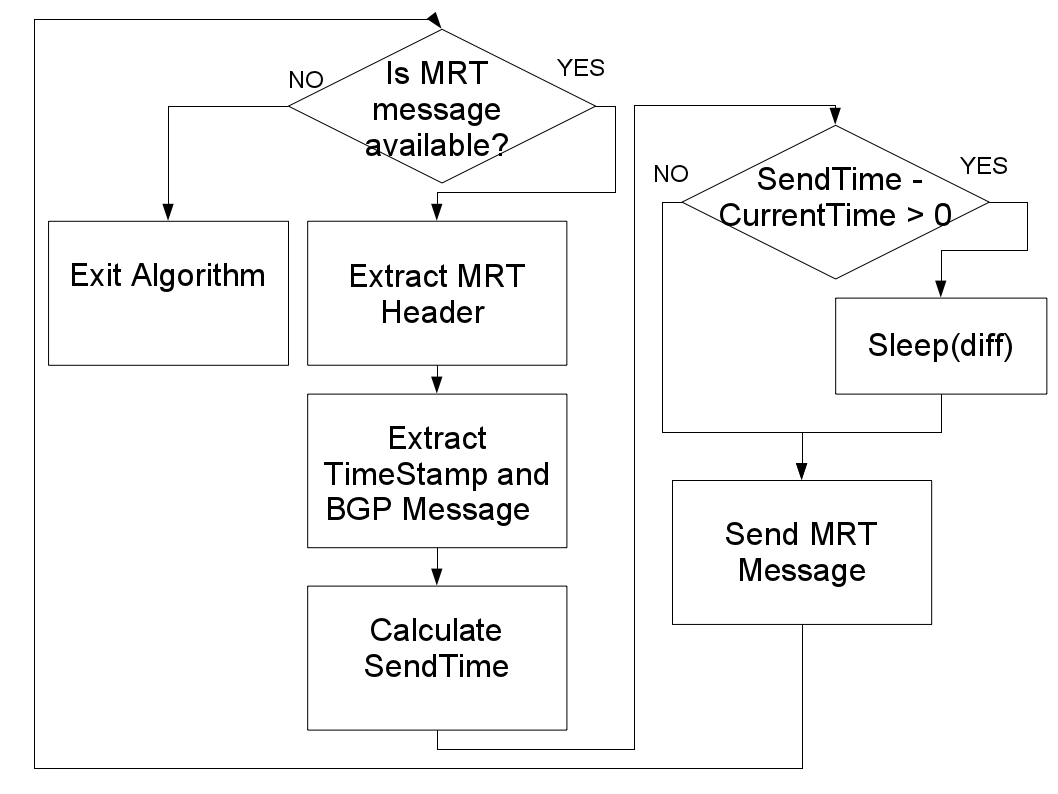
\includegraphics[scale=0.30]{figs/pacing.png}
%\caption{An overview of Timeframing Algorithm.}
%\label{pacingfig}
%\end{figure}

The MRT unit sends the MRT messages using \emph{timeframing} algorithm. Each MRT message in the MRT file has a timestamp. The timestamp in MRT header was created in the past, when the BGP message appeared at the third party.   To play the MRT messages according to the timestamp in the MRT header,  MRT unit calculates the  time shift value or,  simply, the \emph{offset}. The offset helps to adjust the time when message need to be sent. The offset is calculated as the difference in local time and the timestamp from the the first MRT message. Thus, by introducing the offset value, each MRT message requires an approximation of the \emph{sendtime}.  The sendtime indicates  the current send time of the MRT message. The sendtime is calculated as the sum of  timestamp from MRT header and the offset value.   In order to play the MRT messages at the right speed, the MRT unit compares the calculated \emph{sendtime} and the current local time. If the difference is bigger than 0, MRT unit will sleep for the difference time and only then send the MRT message.

In order to provide valid MRT data, the timeframing algorithm perform sanity check over the MRT messages. In particular, it extracts MRT header values from the MRT message and checks the data validity.  For example, a length value of BGP message in MRT header should not be bigger than the BGP message maximum size (4096 bytes). The type value in MRT header need to be equal to one from the MRT draft document.   The details of values and it's sanity check functions   are  described in the \emph{playMRT()} function design. 

The timeframing algorithm include the \emph{mrtplayer.c} and the \emph{mrtplayer.h} library files. The \emph{mrtplayer.h} is a header file that used for function declaration. The \emph{mrtplayer.c} file has source code of functions that are used in the timeframing algorithm. The \emph{mrtplayer.c} includes the  following functions: 

\begin{enumerate}


\item{\textbf{playMRT() function} }

\textbf{Definition:}  
\begin{verbatim}
int playMRT(File *p, int socket);
\end{verbatim}

\textbf{Purpose:}  playMRT() function reads the MRT file, extracts MRT messages and send them to the socket. 

\textbf{Inputs:} the MRT file descriptor, the socket file descriptor.

\textbf{Return values:}

playMRT() function has following return values: 

\begin{itemize}
\item{0: success. Function was executed successfully. }
\item{1: failure. Problem in opening the file descriptor.}
\item{2: failure. The MRT header read is less then 12 bytes.}
\item{3: failure. The MRT header read failed.}
\item{4: failure. Sanity check for timestamp value in MRT header failed}
\item{5: failure. Sanity check for type value in MRT header failed.}
\item{6: failure. Sanity check for subtype value in MRT header failed.}
\item{7: failure. Sanity check for length value in MRT header failed.}
\item{8: failure. The BGP message read is less then the length  bytes value.}
\item{9: failure. The BGP message read failed. }
\item{10: failure. Send of MRT header failed.}
\item{11: failure. Send of BGP message failed.}
\end{itemize} 

\textbf{Functionality:}

\begin{enumerate}
  \item{The playMRT() function checks if the MRT file is open. The playMRT() function check if file descriptor is not equal  to \emph{NULL}, otherwise returns 1.}
  \item{The playMRT() function reads 12 bytes of the MRT header from the file descriptor.  The MRT header is a structure that has four values: \emph{ u\_int32\_t timestamp}, \emph{u\_int16\_t type}, \emph{u\_int16\_t subtype}, \emph{u\_int32\_t length}. The  playMRT() call \emph{fread()} system function to read the data. \emph{fread()} function return the number of items successfully read. playMRT() function checks the return value:  }
  \begin{itemize}
  \item{\emph{fread} returns 12.  No problem occurred. }
  \item{\emph{fread} returns value between 1 and 11. The end of the file is reached or error occurred. The  playMRT() function returns 2.}
  \item{\emph{fread} returns 0. Error occurred. The  playMRT() function returns 3.}
  \end{itemize}

  \item{The playMRT() function performs sanity check for four values in MRT header.}
  \begin{itemize}
    \item{The playMRT() calls internal function \emph{checkTimestamp()} function.  \emph{checkTimestamp()} function takes \emph{ u\_int32\_t timestamp} in input. The  playMRT() function check the return value from \emph{checkTimestamp()} function. Return value of  0  means sanity check for timestamp succeed. If \emph{checkTimestamp()} function returns 1, sanity check failed and the  playMRT() function returns 4. }
    \item{The  playMRT() calls internal function \emph{checkType()} function.  \emph{checkType()} function takes \emph{u\_int16\_t type} in input. The  playMRT() function check the return value from \emph{checkType()} function. Return value of  0  means sanity check for type succeed. If \emph{checkType()} function returns 1, sanity check failed and the  playMRT() function returns 5. }
     \item{The  playMRT() calls internal function \emph{checkSubType()} function.  \emph{checkSubType()} function takes \emph{u\_int16\_t type} and \emph{u\_int16\_t subtype} in input. The  playMRT() function check the return value from \emph{checkSubType()} function. Return value of  0  means sanity check for subtype succeed. If \emph{checkSubType()} function returns 1, sanity check failed and The  playMRT() function returns 6. }
     \item{The  playMRT() calls internal function \emph{checkBGPlength()} function.  \emph{checkBGPlength()} function takes \emph{u\_int32\_t length} in input. The  playMRT() function check the return value from \emph{checkBGPlength()} function. Return value of  0  means sanity check for length succeed. If \emph{checkBGPlength()} function returns 1, sanity check failed and The  playMRT() function returns 7. }
  \end{itemize}
  
  \item{The  playMRT() function  calls \emph{ntohl()} system function to convert the value of length in MRT header file from  network byte order to host byte order.  }
  \item{The  playMRT() function reads \emph{N} bytes of BGP message from the file descriptor.  The \emph{N}  is the converted value of length in MRT header.   The  playMRT() calls \emph{fread()} system function to read the data. \emph{fread()} function return the number of items successfully read. The  playMRT() function checks the return value:  }
  \begin{itemize}
  \item{\emph{fread} returns \emph{N}.  No problem occurred. }
  \item{\emph{fread} returns value between 1 and \emph{N}. The end of the file is reached or error occurred. The  playMRT() function returns 8.}
  \item{\emph{fread} returns 0. Error occurred. The  playMRT() function returns 9.}
  \end{itemize}
  
  \item{The  playMRT() function  calls \emph{ntohl()} system function to convert the value of timestamp in MRT header from network byte order to host byte order. }
  \item{The  playMRT() function calculates the \emph{offset} for the timeframing algorithm. The offset is calculated as the difference of current local time and the timestamp value from  the first MRT message.  The offset value is calculated once and it never should be changed.}
  \item{The  playMRT() function calculates the \emph{sendtime} for the MRT message. The sendtime is the sum of the timestamp value in MRT header and the offset value. }\
  \item{The  playMRT() function calculates the \emph{M} value. The \emph{M} is the difference of local time and sendtime. The \emph{M} value is used to check if MRT message is ready to be sent. If the \emph{M} value is bigger than 0,  The  playMRT() uses the sleep function with \emph{M} seconds.}
  \item{The  playMRT() function uses \emph{send()} function to send  MRT header and BGP message in the socket. \emph{send()} function is called twice.  First, to send the MRT header. Second, to send the BGP message.  Upon successful completion, \emph{send()} shall return the number of bytes sent. Otherwise, -1 shall be returned. The  playMRT() function checks the return value  of \emph{send()} function:}
   \begin{itemize}
  \item{For MRT message, \emph{send()} returns 12.    No problem occurred. }
  \item{For MRT message, \emph{send()} return -1. Error occured. The  playMRT() function returns 10.}
  \item{For BGP message, \emph{send()} returns \emph{N}, where \emph{N} is the length value in MRT header. No problem occurred.}
  \item{For BGP message, \emph{send()} returns -1. Error occured.The  playMRT() function returns 11. }
  \end{itemize}
  
  \item{Upon successful sent of MRT header and BGP message, the  playMRT() function continues to read the rest of file and use the algorithm described above. The  playMRT() function extracts MRT header and BGP message until it reaches the end of the file and, in success,  it returns 0.}

\end{enumerate} % functionality

\item{\textbf{checkTimestamp() function}}

\textbf{Definition:}  
\begin{verbatim}
int checkTimestamp(u_int32_t timestamp);
\end{verbatim}

\textbf{Purpose:}  sanity check for timestamp value.  checkTimestamp() function verifies if the input  timestamp value belongs to the range of the 0 (unix time beginning) and the current unix timestamp.

\textbf{Inputs:} the timestamp value from the MRT header structure.

\textbf{Return values:}
\begin{itemize}
\item{0: success. Function was executed successfully. }
\item{1: failure. Sanity check failed.}
\end{itemize} 

\textbf{Functionality:}

\begin{enumerate}
\item{checkTimestamp() function uses \emph{ntohl()} system function to convert the timestamp value from  network byte order to host byte order.}
\item{checkTimestamp() function checks if the the converted timestamp value is bigger the 0 and less than the current time.  If timestamp value is in the range of (0;current time),  checkTimestamp() function returns 0. Otherwise, it returns 1.}
\end{enumerate}



\item{\textbf{checkType() function}}

\textbf{Definition:}  
\begin{verbatim}
int checkType(u_int16_t type);
\end{verbatim}

\textbf{Purpose:}  sanity check for type value.  checkType() function verifies if the input  type value is equal to at least one type value that defined in MRT draft document. 

\textbf{Inputs:} the type value from the MRT header structure.

\textbf{Return values:}
\begin{itemize}
\item{0: success. Function was executed successfully. }
\item{1: failure. Sanity check failed.}
\end{itemize} 

\textbf{Functionality:}

\begin{enumerate}
\item{checkType() function uses \emph{ntohs()} system function to convert the type value from  network byte order to host byte order.}
\item{checkType() function checks if the the converted type value is equal to one of the following type value:  11 (OSPFv2 type), 12  (TABLE\_DUMP type), 13 (TABLE\_DUMP\_V2 type), 16 (BGP4MP type), 17   (BGP4MP\_ET type), 32   (ISIS type), 33   (ISIS\_ET type), 48   (OSPFv3 type), 49    (OSPFv3\_ET type). In success, checkType() function returns 0. Otherwise, it returns 1.}
\end{enumerate}

\item{\textbf{checkSubType() function}}


\textbf{Definition:}  
\begin{verbatim}
int checkSubType(u_int16_t type, u_int16_t subtype);
\end{verbatim}

\textbf{Purpose:}  sanity check for subtype value.  checkSubType() function verifies if the   subtype value and the type value match to at least one category of subtype and type values  in MRT draft document. 

\textbf{Inputs:} the type value and the subtype value from the MRT header structure.

\textbf{Return values:}
\begin{itemize}
\item{0: success. Function was executed successfully. }
\item{1: failure. Sanity check failed.}
\end{itemize} 

\textbf{Functionality:}

\begin{enumerate}
\item{checkSubType() function uses \emph{ntohs()} system function to convert the type value from  network byte order to host byte order.}
\item{checkSubType() function uses \emph{ntohs()} system function to convert the subtype value from  network byte order to host byte order.}
\item{Not all types have a subtype, checkType() check specific  subtypes for the following types:  12  (TABLE\_DUMP type), 13 (TABLE\_DUMP\_V2 type), 16 (BGP4MP type), 17   (BGP4MP\_ET type).   For type  12, checkSubType() function checks if subtype if equal to 1  or 2. For type 13, checkSubType() checks if subtype is equal to 1, 2, 3, 4, 5 or 6. For type  16 or 17, checkSubType() function checks if subtype if equal  0, 1, 2, 3, 4, 5, 6 or 7.  For other types, checkSubType() does not check subtype value. In success checkSubType() return 0, in failure 1. }

\end{enumerate}




\item{\textbf{checkBGPlength() function} }

\textbf{Definition:}  
\begin{verbatim}
int checkBGPlength(u_int32_t length);
\end{verbatim}

\textbf{Purpose:}  sanity check for length value.  checkBGPlength() function verifies if the input  length value is bigger then 0 but less then the max size of BGP message (4096 bytes).

\textbf{Inputs:} the length value from the MRT header structure.

\textbf{Return values:}
\begin{itemize}
\item{0: success. Function was executed successfully. }
\item{1: failure. Sanity check failed.}
\end{itemize} 

\textbf{Functionality:}

\begin{enumerate}
\item{checkBGPlength() function uses \emph{ntohl()} system function to convert the length value from  network byte order to host byte order.}
\item{checkBGPlength() function checks if the the converted length value is bigger the 0 and less than 4096. In success, it returns 0. In failure, it returns 1.}
\end{enumerate}

\item{\textbf{MRTconnect() function} }

\textbf{Definition:}  
\begin{verbatim}
int MRTconnect(char *hostname);
\end{verbatim}

\textbf{Purpose:}  MRTconnect() function creates a socket connection to the given hostname with PORT 7777.

\textbf{Inputs:} hostname string.

\textbf{Return values:}
\begin{itemize}
\item{N:  success. Function returns a non-negative socket file descriptor.}
\item{-1: failure. The \emph{getaddrinfo()} function failed.}
\item{-2: failure. The \emph{socket} function failed.} 
\item{-3: failure. The \emph{connect} function failed.}
\end{itemize} 



\textbf{Functionality:}
  \begin{enumerate}
  \item{The MRTconnect() function identifies specified hostname. The MRTconnect() function uses the \emph{getaddrinfo()} system function. The \emph{getaddrinfo()} takes four inputs: the given hostname, the port number,   \emph{hints addrinfo} and \emph{res addrinfo} data structures. The hostname is given hostname from the input. \emph{getaddrinfo()} uses port 7777 to connect to hostname. The \emph{hints addrinfo} input points to an \emph{addrinfo} structure that specifies criteria for selecting the socket address structures  returned  in  the  list  pointed  to  by  \emph{res addrinfo}.  The MRTconnect() function checks the return value from the \emph{getaddrinfo()} function:}
  \begin{itemize}
  \item{Upon successful completion, \emph{getaddrinfo()} returns 0. }
  \item{\emph{getaddrinfo()} returns non-zero error codes that correspond to failure . The MRTconnect() function returns -1. }
  \end{itemize}
  
  \item{The MRTconnect() function uses the \emph{res addrinfo}  data structure to create a socket connection. The MRTconnect() function uses the \emph{socket()} system function to get the socket file descriptor.  The \emph{socket} function takes the \emph{ai\_family}, \emph{ai\_socktype} and \emph{ai\_protocol} values from the \emph{res addrinfo} data structure.  The MRTconnect() function checks the return value from \emph{socket()} function:  }
  \begin{itemize}
  \item{Upon  successful  completion, \emph{socket()} returns a non-negative integer (socket file descriptor.)}
  \item{In a failure, \emph{socket()} function returns -1. The MRTconnect() returns -2. }
  \end{itemize}
  
  \item{The MRTconnect() function uses \emph{connect()} function to establish a connection. The \emph{connect} function attempts to make a connection on a socket. The function takes the following arguments: the socket file descriptor, \emph{ai\_addr} and \emph{ai\_addrlen} values from 
  \emph{res addrinfo} data structure. The MRTconnect() function checks the return value from the \emph{connect} function: }
  \begin{itemize}
  \item{Upon successful completion, \emph{connect()} function return 0.}
  \item{In a a failure, -1 is returned. The main() function closes the socket file descriptor and returns -3. }
  \end{itemize}
   \item{The MRTconnect() function return the socket file descriptor.}
\end{enumerate}



\end{enumerate} %function list definition



% The Timeframing method allows to play the MRT messages at the speed they were created.  Figure \ref{pacingfig} shows the design of timeframing algorithm.  It uses MRT data files in input and  starts with repeat loop that checks if MRT messages are available. If there are no MRT messages left, algorithm exist. Otherwise, timeframing method  reads MRT messages and it extracts the MRT header with timestamp and the BGP message.   Then, it calculates the \emph{sendtime} that is used to verify if the MRT message is ready to be sent.   If the difference in \emph{sendtime - currenttime} bigger then 0, it sleeps the time difference. For example, if current time is \emph{8:00:00 am} and calculated \emph{sendtime} of MRT message is \emph{8:00:05 am}, timeframing algorithm will sleep for 5 seconds.     Once MRT message is sent to BGPmon application, the algorithm continues operate  with next available MRT message from the MRT file.  





\subsubsection{MRT Feeder Design Overview}
\label{sec:mrtfeederdesign}

The MRT feeder is an application that designed to inject MRT messages into the BGPmon Test Framework. It uses the \emph{timeframing} algorithm to send the MRT messages from the provided MRT file.  The MRT feeder application include the \emph{mrtfeeder.c} and the \emph{mrtfeeder.h} files.  The \emph{mrtfeeder.h} is a header file that used for function declarations. The \emph{mrtfeeder.c} is a source code file of MRT feeder application.  Also, the MRT feeder application includes the  \emph{mrtplayer.h} header file and use the functions defined in timeframing library. \emph{mrtplayer.c} includes the  following functions: 

\begin{enumerate}

\item{\textbf{main() function} }

\textbf{Definition:}  
\begin{verbatim}
int main(int argc, char **argv)
\end{verbatim}

\textbf{Purpose:} the main() function starts MRT feeder application. 

\textbf{Inputs:} \emph{argc} and \emph{argv} values. The argc is a count of the arguments supplied to the program and the argv is an array of pointers to the strings which are the arguments to main function. The arguments are passed to the program by the host system's command line interpreter. 

\textbf{Return values:}

The MRT feeder  uses the return values that are defined in \emph{stdlib.h} system library:
\begin{itemize}
\item{EXIT\_SUCCESS. function execution is  successful. }
\item{EXIT\_FAILURE: function execution failed.}
\end{itemize} 

\textbf{Error log printing:}

main() function uses the \emph{perror()} system function to print error messages. \emph{perror()} function produces a message on the standard error output, describing the last error encountered during a call to a system or library function.

\textbf{Functionality:}

\begin{enumerate}
  \item{The main() function starts with parsing the arguments that are provided by the user. The  main() function uses the \emph{getopt()} system function. The \emph{getopt} is design to  break  up  (parse)  options  in command lines for easy parsing by shell procedures, and to check for legal    options.  MRT feeder \emph{geptop()} function takes three inputs. First, the [-f filename] option is designed to use provided filename from the arguments.  Second, the [-d hostname] option is designed to use provided hostname from the arguments.  Third, the [-u] options is designed to set the \emph{keepTCP} integer to 1. Details of [-u] option are discussed further.  The main() function runs the while loop with true condition and checks the return value from the \emph{getopt()} function. Once the \emph{getopt} parsed the command line, it returns -1. The  main() function stops the while loop.}
  
  \item{The  main() function checks the filename extension. The user of the MRT feeder may provide archived MRT files in input. The  main() function uses the \emph{strtok()} system function. The  strtok()  function parses a string into a sequence of tokens. For a given filename, \emph{strtok()} function will lookup for a delimiter. The  main() function uses ".bz2" string as a delimiter. \emph{strtok()} inputs the filename and the delimiter and returns following values:    }
  \begin{itemize}
  \item{A NULL pointer: strtok() function could not find any token that matches the given delimiter. The  main() function will not extract the filename.}
  \item{A pointer to the last token found in filename. This means that provided filename is an archive and it need to be extracted. The main() function use \emph{system()} function to extract the filename. \emph{system()} function executes  a  command  specified  in input by calling \emph{/bin/sh -c} command. \emph{system()} function uses two inputs: the \emph{bunzip2} tool to extract the MRT file and the given filename.  The  main() function checks the return value of  \emph{system()}  function:}
  \begin{itemize}
  \item{\emph{system} function returns -1. This an error. The  main() function exits with EXIT\_FAILURE value}
   \item{\emph{system} function returns the return status of the execution of \emph{bunzip2} command. \emph{bunzip2} returns 0 for a normal exit and 1 for  environmental problems (file not found, etc.)  In case of 1,  the  main() function exits with EXIT\_FAILURE. In case or 0, filename was successfully extracted.}
  \end{itemize}  
  
  \end{itemize}

  \item{The  main() function opens the filename. The  main() function uses the \emph{fopen()} system function to open the filename. \emph{fopen()} function takes two inputs, first the given filename and second, the mode. The  main() function uses "rb" mode to open binary MRT file for a read. The  main() function checks the return value of \emph{fopen} function. }
  \begin{itemize}
  \item{\emph{fopen} function returns a NULL pointer. An error occured. The  main() function exits with EXIT\_FAILURE value.}
  \item{Upon successful completion \emph{fopen} function returns  the file descriptor. }
  \end{itemize}
  
  
  \item{The  main() function  uses the \emph{MRTconnect()} function from the \emph{mrtplayer.c} library. \emph{MRTconnect()} takes the hostname in input and returns the socket file descriptor. The main() function checks the return value from the \emph{playMRT()} function.}
   \begin{itemize}
  \item{In a success, the \emph{MRTconnect()} function returns a non-negative value (the socket file descriptor). }\
   \item{In a failure, the \emph{MRTconnect()} function returns a error number. The main() function uses the \emph{switch()} system function to print the corresponding error  message. In a failure, the main() function closes the file descriptor and exits with EXIT\_FAILURE value.}
  \end{itemize}
  
    
  \item{The  main() function  uses the \emph{playMRT()} function from the \emph{mrtplayer.c} library. The  \emph{playMRT()} function takes two inputs: the file descriptor and the socket file descriptor. The \emph{playMRT()} function send the  MRT data via socket connection. The main() function checks the return values from the \emph{playMRT()} function. The main() function checks the return value from the \emph{playMRT()} function.}
  \begin{itemize}
  \item{In a success, the \emph{playMRT()} function returns 0. }\
   \item{In a failure, the \emph{playMRT()} function returns a error number. The main() function uses the \emph{switch()} system function to print the corresponding error  message. In a failure, the main() function closes the file descriptor,  the  socket file descriptor and exits with EXIT\_FAILURE value.}
  \end{itemize}
  
  
  \item{After the the main() function sent the MRT file, it  checks the \emph{keepTCP} integer value.    The \emph{keepTCP} value is set to 1 if  the MRT fetcher application was started with \emph{-u} options at the command line. In the design of MRT feeder, this option is created to leave TCP connection open until the user types "exit" in command line. }
  \begin{itemize}
  \item{If \emph{keepTCP} is enabled, the main() uses a while loop with true condition and it uses  two functions: \emph{fgets()} and \emph{strcmp()}.  In the while loop the main()function calls \emph{fgets} to read the data from the command line.  The \emph{fgets} function has three inputs: the \emph{char buffer}, the size of the char buffer and the source of the stream.  The main() function define the char buffer \emph{buf} with size of 100 bytes. The source of the stream is \emph{stdio}.  The main() function  checks  the \emph{fgets()} function return values.}
  \begin{itemize}
  \item{On error, the \emph{fgets()} function return NULL. The main() function closes}
  \item{Upon successful completion, \emph{fgets()} returns the read characters from command line. }
  \end{itemize}
  \item{In the while loop,  the main() function use the \emph{strcmp()} function. The \emph{strcmp()} function  compares the two input strings. The first input string is string from the char buffer that \emph{fgets} provides. The second string is defined "exit" string.  The main() function checks the \emph{strcmp()} function return values.  }
  \begin{itemize}
    \item{If two strings are equal, the \emph{strcmp()} function returns 0. The main() function breaks the while loop. }
  \item{If two strings are different, the \emph{strcmp()} function returns the byte difference between two strings.  The main() function continues to loop the while loop  and reads the input from the command line.}
  \end{itemize}
  \end{itemize}
  
  \item{The main() function uses \emph{close()} function to close the file descriptor and the socket file descriptor. Lastly, the main() function will exit with EXIT\_SUCCESS value. }
  

\end{enumerate}



\end{enumerate} %function list definition


%\begin{figure}
%\centering
%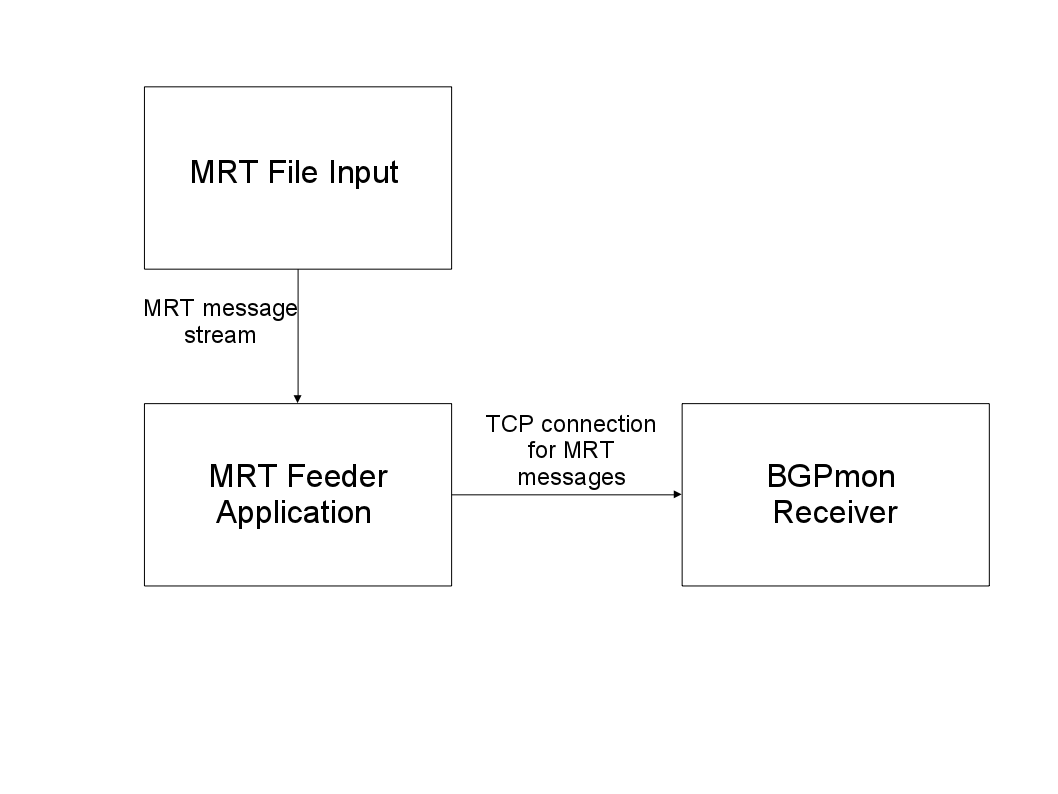
\includegraphics[scale=0.30]{figs/mrtfeeder-design.png}
%\caption{An overview of MRT Feeder application.}
%\label{feederdesignfig}
%\end{figure} 

%The MRT feeder is an application that designed to inject MRT messages into the BGPmon Test Framework.  Figure \ref{feederdesignfig} shows the design of  MRT feeder application. Figure shows the inputs and the outputs of the system.  The MRT File Input provides MRT files. In case of MRT File Input provides archived MRT files, the MRT feeder extracts the MRT file.  The BGPmon application is receiver that receives MRT messages.    The MRT feeder takes the MRT file from MRT File Input instance, extracts MRT messages and send them to BGPmon application over TCP connection.  

%\begin{figure}
%\centering
%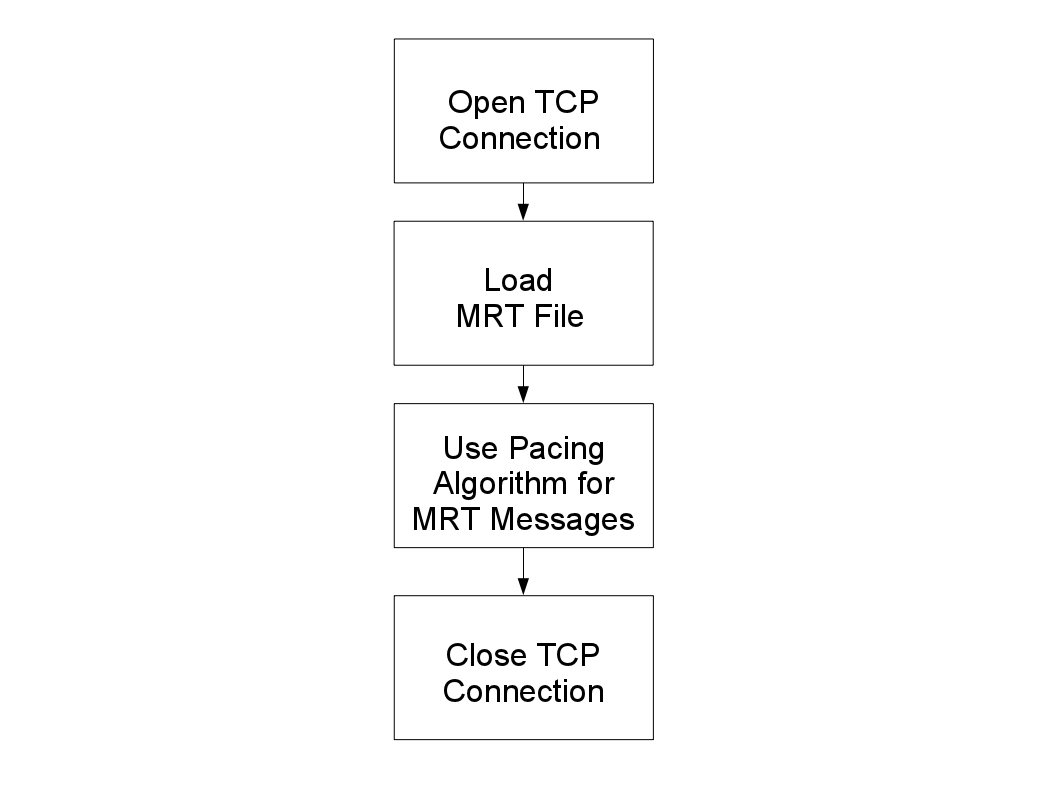
\includegraphics[scale=0.30]{figs/mrtfeeder-flow.png}
%\caption{MRT Feeder Data Flow Overview.}
%\label{feederflowfig}
%\end{figure}

%Figure \ref{feederflowfig} shows the data flow in MRT feeder. There are few simple components that are used in the MRT Feeder.   When the MRT Feeder application is executed, first it opens a TCP connection to BGPmon receiver.  Second, the MRT Feeder opens the MRT file from the input. Third, the MRT feeder uses \emph{timeframing} algorithm to extract and send MRT messages to BGPmon. \emph{Timeframing} alrotihgm is described in Section \ref{sec:timeframing}.  MRT feeder plays MRT messages at the same speed as they were received at the third party.  Once the MRT feeder reaches the end of the MRT file, it closes TCP connection to BGPmon receiver. 

%The MRT feeder has following running options:


%\begin{verbatim}
%$ mrtfeeder [-u] [-f filename] [-d host]
%\end{verbatim}
%   where:
%  \begin{itemize}
%  \item{\emph{-u} is an options that force MRT feeder to keep TCP connection when the MRT feeder %sent all MRT messages.}
%  \item{\emph{-f filename} is an MRT file name.  The user may provide archived file name. The MRT %feeder looks into the file name and detects if MRT file need to be extracted. }
%  \item{\emph{-d host} is name of the host that runs BGPmon receiver. }
%  \end{itemize}  
  
  
  
%The MRT feeder works as follows. The MRT feeder opens a single TCP connection to BGPmon receiver.  The MRT feeder takes the MRT file name and opens it to read MRT messages.  For each MRT message, the MRT feeder extracts the timestamp and the BGP message.   MRT feeder uses the \emph{timeframe} mechanism to send MRT messages.  For instance, if the first  MRT message originated at \emph{8:00:00 am} and the second MRT message at \emph{8:00:03},  MRT fetcher will send the first MRT message, wait for 3 seconds and send the second MRT message. \emph{Timeframe} mechanism allows the tester of the framework to play MRT messages at the right speed.  Once the all MRT messages from the MRT file are sent,  MRT feeder has an option (\emph{-u} flag in input)  to close TCP connection  or leave  it open until the user of the framework terminates it manually. This option helps in debugging BGPmon application.
 



\subsubsection{MRT Fetcher Design Overview}
\label{sec:mrtfetcherdesign}

%The MRT feeder application include the \emph{mrtfeeder.c} and the \emph{mrtfeeder.h} files.  The \emph{mrtfeeder.h} is a header file that used for function declarations. The \emph{mrtfeeder.c} is a source code file of MRT feeder application.  Also, the MRT feeder application includes the  \emph{mrtplayer.h} header file and use the functions defined in timeframing library. \emph{mrtplayer.c} includes the  following functions: 

The MRT fetcher application is designed to run in the \emph{collector mode}. The MRT fetcher application goal is to imitate the behaviour of the routing collector. The routing collector sends two types of data: the MRT table snapshot that provides a set of  routing tables from connected peers and sequential set of MRT update messages that update the routing information.  The  The MRT fetcher application is designed to send MRT data from the existing routing collectors.  In particular, it uses the RouteViews collector's archives to fetch the MRT data. The MRT fetcher takes two unix timestamps: the \emph{start time} and the \emph{end time}. The \emph{start time} specifies the time when MRT fetcher sends the MRT messages. The  \emph{end time} specifies the time when the MRT fetcher stops sending the MRT data.   The RouteViews collectors provides the MRT tables that are generated every two hours and the MRT update files that are generated every 15 minutes. The MRT fetcher application goal is to send the MRT data that originated between \emph{start time} and the \emph{end time}.  

The MRT fetcher is designed in following way. First,  the MRT fetcher calculates the \emph{table time}. The \emph{table time} is unix time that specifies the most recent (in the range of 2 hours) MRT table snapshot. The \emph{table time}  is calculated as the nearest integer divisible by 7200. For example, if the input \emph{start time} is equal to \emph{1317203100} (Sept 22, 2011, 9:45:00 am), the \emph{table time} is calculated as  integral part of \emph{star time} divided by 7200  and  multiplied by 7200. The calculation gives the \emph{table time} to be equal to 1317196800 (Sept, 22, 2011, 8:00:00 am) and it gives the most recent  unix time of MRT table file. The MRT fetcher downloads  the proper MRT table file from the RouteViews collector archive.   The MRT fetcher extracts the archive and use \emph{send()} function  to  send the MRT table file via socket connection.  Second,  the MRT fetcher is designed to play MRT  update messages at the right speed that corresponds to specified \emph{start time} and \emph{end time}.  In the example above, the MRT fetcher is 1 hour and 45 minutes below the requested \emph{start time}. In order to get to the MRT update messages  originated at \emph{starttime}, the MRT fetcher sends MRT update messages starting from \emph{table time} and ending the \emph{start time} values. The MRT fetcher does not apply timeframing algorithm to those messages. The MRT fetcher fetches and  sends 7 MRT update files that fall in the 1 hour and 45 minutes gap.   Third, the MRT fetcher is ready to play the messages that originated from \emph{start time} and ends on the \emph{end time}. The MRT fetcher fetches each MRT update message from the RouteViews archive and sends it using the \emph{timeframing} algorithm.

%In addition, proposed design has some number of  challenges. In particular,

%In MRT fetcher, the  fetching of MRT data from RouteViews archive takes some amount of time. Also, extracting of MRT data files takes time too. 
%In one hand, possible delays in retrieving and unzipping the data may create time gap between the MRT update files.  Every update message file from RouteView archive is a set of MRT messages. 
The \emph{timeframing} algorithm plays the messages at the right speed. This means that the set of MRT messages from the MRT update file is spread across 15 minutes interval. In the \emph{timeframing}  algorithm two or more MRT messages may have a few seconds delay. And \emph{timeframing} algorithm calculates the time time when those messages need to be send.  In MRT fetcher, fetching the MRT file and extracting the MRT file takes the time. The MRT fetcher creates a small timing gap between the two MRT files. This gap is measurable in order of few seconds and does not affect the overall speed of sending MRT files.    

 

\begin{enumerate}

\item{\textbf{main() function} }

\textbf{Definition:}  
\begin{verbatim}
int main(int argc, char **argv)
\end{verbatim}

\textbf{Purpose:} the main() function starts MRT fetcher application. 

\textbf{Inputs:} \emph{argc} and \emph{argv} values. The argc is a count of the arguments supplied to the program and the argv is an array of pointers to the strings which are the arguments to main function. The arguments are passed to the program by the host system's command line interpreter. 

\textbf{Return values:}

main() function uses the return values that are defined in \emph{stdlib.h} system library:
\begin{itemize}
\item{EXIT\_SUCCESS. function execution is  successful. }
\item{EXIT\_FAILURE: function execution failed.}
\end{itemize} 

\textbf{Error log printing:}

The main() uses the \emph{perror()} system function to print error messages. \emph{perror()} function produces a message on the standard error output, describing the last error encountered during a call to a system or library function.

\textbf{Functionality:}
NEEDS WORK: section requires a lot details.
\begin{enumerate}



\item{The main() uses the \emph{getopt()} function to parse command line. }

\item{The main() checks the RouteView collector name. Based on collector name string, the main() function chooses the right URL to fetch the MRT data.  }

\item{The main() function calls the \emph{MRTconnect()} function twice to establish two TCP connecitons. One is designed to send MRT table file, another - to send the MRT update file.}

\item{The main() function uses the starttime from the input and  calculates the \emph{table time}. }

\item{The main() uses the \emph{libcurl} library to fetch the MRT table file from the Routeview collector.  The \emph{libcurl} saves archive in \emph{/home/bgpmoner/Development/bgpmon-dev/test/mrt\_harness/data} folder. }

\item{The main() function extracts the MRT table file. }
\item{The main() function sends the MRT file using the first socket file descriptor.}
\item{The main() function closes the socket file descriptor.}

\item{The main() function uses three timestamps variables: the \emph{table timestamp}, the \emph{start time} and the \emph{end time}.  For a range of [\emph{table timestamp; start time}), the main() function fetches the corresponding  MRT update file, extract it and use \emph{send()} system function to write the data to the socket file descriptor. If [\emph{table timestamp; start time}) includes many MRT update files, the main() function will repeat the previous step until the last MRT update that falls within the range. For a range of [\emph{start time; end time}), the main() function fetches the  corresponding MRT update file, extract it and use the \emph{timeframing} algorithm to send MRT messages at the right speed.  If [\emph{ start time; end time}) includes many MRT update files, the main() function will repeat the previous step until the last MRT update that falls within the range. }

% The \emph{MRT table timestamp} is the unix timestamp of MRT table file. The \emph{starttime} and the \emph{endtime} are the unix timestampes that come from the MRT fetcher startup arguments.  The main() function use \emph{for loop} to send the MRT update files. The \emph{for loop} uses the timestamps described before.   In the \emph{for loop}, the start index starts from \emph{MRT table timestamp}, the end condition is the \emph{endtime},  the increase index is 900 seconds (15 minutes) interval between each MRT update file.    For each index in the \emph{for loop}, the main() function calculates the name of the MRT update file.  Then, it uses \emph{libcurl} to download the file.  Each downloaded file need to be extracted.     
%The \emph{for loop} has an \emph{if} statement that checks if index becomes bigger then the \emph{starttime} from the input. 




\item{For each of MRT update files, the main()  function uses the \emph{libcurl} library to fetch the MRT update  messages. }


\item{The main() function closes the socket file descriptor.}




\end{enumerate}

\end{enumerate}



%\begin{figure}
%\centering
%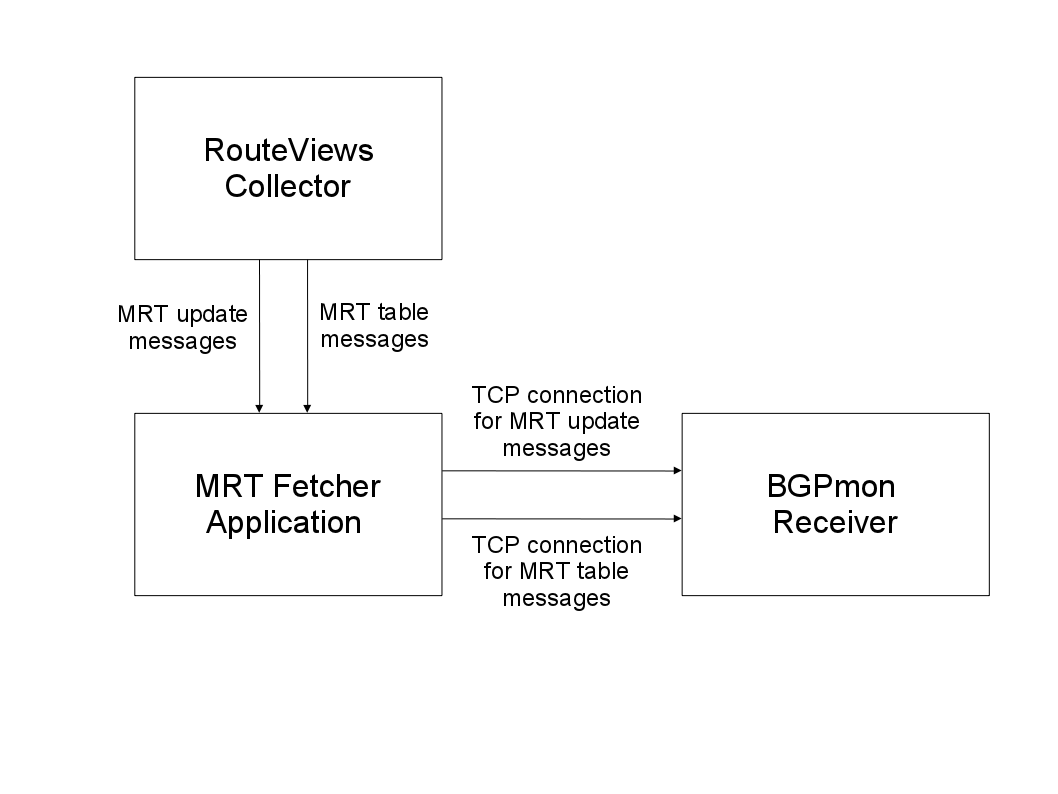
\includegraphics[scale=0.30]{figs/mrtfetcher-design.png}
%\caption{An overview of MRT Fetcher application.}
%\label{fetcherdesignfig}
%\end{figure}

%The MRT fetcher application is designed to run in \emph{collector mode}.  The MRT fetcher %application is designed to send MRT data from the existing routing collectors. Figure %\ref{fetcherdesignfig} shows the MRT fetcher design.  It shows inputs and outputs of the system.  
%The MRT fetcher uses the RouteViews collector to as source of the MRT data. The RouteViews %collector provides the MRT update files and the MRT table files.  
%The MRT fetcher extracts the MRT messages from the MRT update files and the MRT table files. 
% The BGPmon application is receiver that receives MRT messages. The top TCP connection shown in %Figure \ref{fetcherdesignfig} is designed to send MRT update messages from the MRT update file.     %The bottom TCP connection is designed to send MRT table messages from the MRT table file. 

%The MRT feeder creates two TCP connection to BGPmon application. One TCP connection is used to send the MRT table messages. Another TCP connection is designed to  send the MRT update messages. 

%\begin{figure}
%\centering
%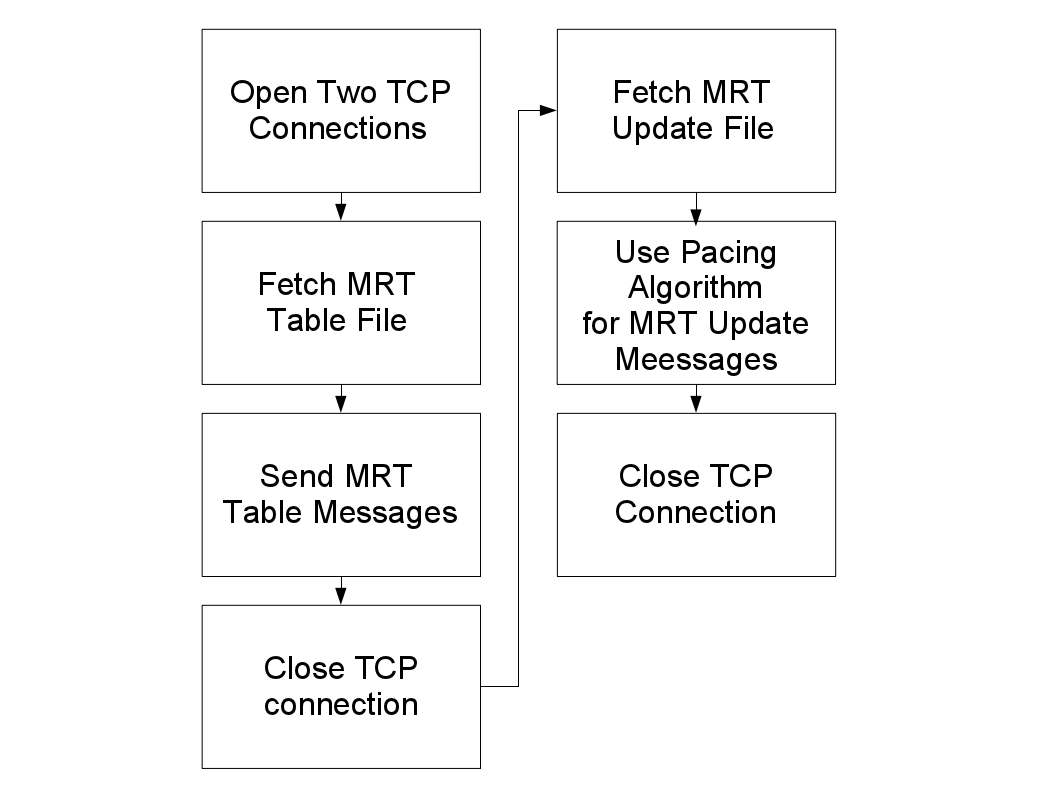
\includegraphics[scale=0.30]{figs/mrtfetcher-flow.png}
%\caption{MRT Fetcher Data Flow Overview.}
%\label{fetcherflowfig}
%\end{figure}

%Figure \ref{fetcherflowfig} shows the data flow in MRT feeder. There are few simple components that are used in the MRT Feeder. First, MRT fetcher opens two  TCP connections to BGPmon application.  Second, the MRT fetcher downloads an archived MRT table file from RouteViews collector. The MRT fetcher extracts the archive and sends the MRT table file to  BGPmon application.  Once the data is sent out, the MRT fetcher closes the TCP connection.  Further, the MRT fetcher downloads an archived MRT update file. It extracts the MRT file and uses \emph{timeframing} algorithm to send MRT messages to BGPmon application.  The \emph{Timeframing} algorithm is discussed in details  in Section \ref{sec:timeframing}. Once the MRT fetcher reaches the end of the MRT update file, it closes TCP connection to BGPmon receiver.   

%The MRT fetcher sends MRT data based on the specified  start time and end time.   The MRT fetcher rounds down the start time and the end time to get the most recent MRT table messages and MRT update messages.   For example,  the user may specify the start time of \emph{Sept 20th, 2011, 9:45 am}  in the MRT fetcher. The RouteViews collector provides the MRT snapshot with MRT table messages every two hours. The MRT fetcher will use \emph{Sept 20th, 2011,  8:00am} MRT snapshot  as the most recent MRT table data source.   Once the MRT table messages are sent, the MRT fetcher will close the first TCP connection and start sending sequence of MRT update messages over the second TCP connection. The RouteViews collector provides the MRT update files with MRT update messages every 15 minutes. The MRT fetcher rounds down the start time and end time for MRT update files. For example, if  the user of the MRT fetcher, assigns a time of \emph{Sept 20th, 2011, 9:45 am} as the start time and \emph{Sept 20th, 2011, 10:10am} as the end time, MRT fetcher will send two MRT update files, first at the time of \emph{Sept 20th, 2011,  9:45 am} and  second at the time of \emph{Sept 20th, 2011, 10:00 am}. 

%The MRT fetcher application is similar to the  MRT feeder application, but it designed to send the MRT files from existing routing collectors. 

  
%The MRT fetcher has following running options:

%\begin{verbatim}
%$ mrtfetcher [-q] [-u] [-c collector] [-s starttime] 
%        [-e endtime]  [-d hostname]
%\end{verbatim}
%where
%\begin{itemize}
%\item{\emph{-q} option instructs MRT fetcher to keep TCP connection when the MRT fetcher sent all %MRT messages.}
%\item{\emph{-u} option instructs MRT fetcher to send the MRT update messages only. This option %skips fetching MRT table files.}
%\item{\emph{-c collector} is used to specify one the RouteView collectors.}
%\item{\emph{-s starttime} is unix timestamp that is used to start sending MRT data.}
%\item{\emph{-e endtime} is unix timestamp that is used to end sending MRT data.}
%\item{\emph{-d hostname} is a name of the host with BGPmon receiver.}
%\end{itemize}


%The MRT fetcher sends two types of MRT data: MRT table files and MRT update files.  The MRT fetcher uses RouteViews collector to fetch the MRT table and the MRT update files. The MRT fetcher creates two TCP connection to BGPmon.  
 
  

% The MRT fetcher is designed to use   \emph{timeframing} algorithm to play MRT messages at the right speed.  The MRT fetcher uses MRT feeder's \emph{timeframing} algorithm described in Section \ref{sec:mrtfeederdesign}.  The MRT fetcher uses \emph{timeframing} for the MRT update messages that originated  between the specified start time and the end time.  For instance,  the tester specified start time of \emph{Sept 20th, 2011, 9:45 am} and end time of \emph{Sept 20th, 2011, 10:10 am}.  First, the MRT fetcher will round down the start time and use the nearest MRT table snapshot at the  \emph{Sept 20, 2011, 8:00 am}.  Second, the MRT fetcher will start sending MRT update files from   \emph{Sept 20th, 2011, 8:00 am} to \emph{Sept 20th, 2011, 9:45 am}. Those MRT update messages will be processed without the timeframing. The MRT update messages from \emph{Sept 20th, 2011, 9:45 am} to \emph{Sept 20th, 2011, 10:10 am} will have the \emph{timeframing} and they will be played at the right speed to the BGPmon receiver.



%The MRT fetcher and MRT feeder have common functionality. For example, both applications are designed to send MRT files to BGPmon receiver. Both application use \emph{timeframing} to play MRT messages at the right speed.  In order avoid  duplicate code, MRT fetcher uses the library functions of MRT feeder. For example, MRT fetcher uses a function from MRT feeder that sends MRT messages over the TCP connection.  


%sends to use already collected MRT files.  The  MRT fetcher use MRT files from the RouteViews archive.  The RouteViews archive provides two types of MRT files: MRT table files and MRT update files. The MRT fetched use MRT table and MRT update files to inject MRT messages into BGPmon instance.  



%MRT fetcher application sends MRT messages in

%* How the Fetcher design looks like?
%* How does it work?  2 tcp connections? 
%* What are the inputs?  What are the outputs? 
%* Options to run ?
%* Timeframing? 
%* How to send updates only? Should be an option. 


%\subsubsection{MRT Analyzer Design Overview}
%\label{sec:mrtfetcherdesign}

%MRT analyzer is a tool that designed to help  in debugging. MRT analyzer outputs a number of %statistics about the peers in MRT file. 
  
%The MRT analyzer has following running options:


%\begin{verbatim}
%$ mrtanalyzer [-c filename] [-d directory]
%\end{verbatim}
%  where:  
%  \begin{itemize}
%  \item{\emph{-c filename} is MRT file. }
%  \item{\emph{-d directoy} is the output directory. MRT analyzer produce output in specified %directory.}
%  \end{itemize}

%The MRT analyzer takes an MRT file as input.   The MRT analyzer uses \emph{bgpdump} tool to extract MRT messages.  The MRT analyzer takes the output from \emph{bgpdump} tool and finds the list of unique peers. The list of peers is stored as \emph{peerlist.txt} in output directory.  For each peer, the MRT analyzer constructs the routing table.  For example, at the time \emph{Sept 22th, 2011, 10:15:00 am} peer \emph{12.0.1.63} received two announce messages with   \emph{11.0.0.0/8} and \emph{13.0.0.0/8} network prefixes. Later, at \emph{Sept 22th, 2011, 10:15:30 am} there was a withdrawn message that removes the \emph{11.0.0.0/8} network prefix. MRT analyzer analyses the list of announced and withdrawn network prefixes  and leave the most recent routes in  table. In example above, \emph{12.0.1.63} peer would have \emph{13.0.0.0/8} prefix in \emph{12.0.1.63\_table.txt} file in output directory. 
 



\section{Labeling Module}
\label{sec:labeling}
Labeling module manages one RIB-IN table associated with a peer if configured and uses the tables to assign labels to updates received from the peer.  In this module, the only configuration is about how to process the BGP updates from peers. It is specified by "labelAction" in peer configuration as shown in Figure \ref{fig:configurationSub}. "labelAction" could be one of these three options:
\begin{itemize}
\item{ \emph{None:} Don't process the updates at all. }
\item{ \emph{RibStore:} Store the updates in RIB-IN tables on a per-peer basis. The peer has its own RIB-IN table if this option is set.}
\item{ \emph{Label:} Store the updates in RIB-IN tables and label the updates based on how they change RIB-IN tables. This option implicitly stores RIB-IN for the peer. }
\end{itemize}
Since the RIB-IN tables are the major memory consumption of BGPmon, one might want to set "labelAction" as "None" if the memory is the major concern. 

Labeling module has a single thread which is a reader of peer queue and a writer of label queue as shown in Figure \ref{fig:architecture}. Main flow has three steps:
\begin{itemize}
\item{ Read the BMF messages from peer queue }
\item{ If the BMF message is a update, then process it based on the "labelAction" configuration. Otherwise, do nothing.}
\item{ Write the processed BMF messages into labeling queue }
\end{itemize}
The detail of main flow logic will be discussed in section \ref{sec:labeling:mainflow}.

\subsection{Data Structure}
Labeling Module uses 2 main data structures(PrefixTable and AttrTable) to maintain the RIB-IN table. As the RIB-IN table is maintained on a per-peer basis, it is natural to make these 2 structures as components of the "Session" structure as we mentioned in section \ref{sec:peering:sessionstructure}.  "PrefixTable" and "AttrTable" are used to store prefixes and attributes in BGP updates respectively. And these 2 tables are inter-linked to make up one RIB-IN table.

\subsubsection{ PrefixTable Structure}
\label{sec:labeling:prefixtable}
In our design it is a hash table that consists of multiple entries. Each entry is a link list of nodes and each node contains a prefix. It has the following six parts.
\begin{itemize}
\item{\emph{prefixCount:} is the number of prefixes are contained in the prefix hash table.}
\item{\emph{tableSize:} is the number of entries in the hash table.}
\item{\emph{occupiedSize:} is the number of occupied entries in the hash table. Occupied entry means it has at least one node. }
\item{\emph{maxNodeCount:} is the max length among all entries in the hash table. The length of one entry indicates how many nodes it contains.}
\item{\emph{maxCollision:} is the max number of nodes one entry is allowed to contain. If one entry contains too many nodes, we need to increase the number of entries in a hash table in order to improve the performance. Basically if maxNodeCount is larger than maxCollision, we need to enlarge the hash table.}
\item{emph{prefixEntries:} is an array of PrefixEntry structures. It contains all the entries of the prefix hash table. For the details of PrefixEntry structure, see Figure \ref{fig:PrefixEntryStruct}.}
\end{itemize}
\begin{figure*}
\centering
\scalebox{0.8}{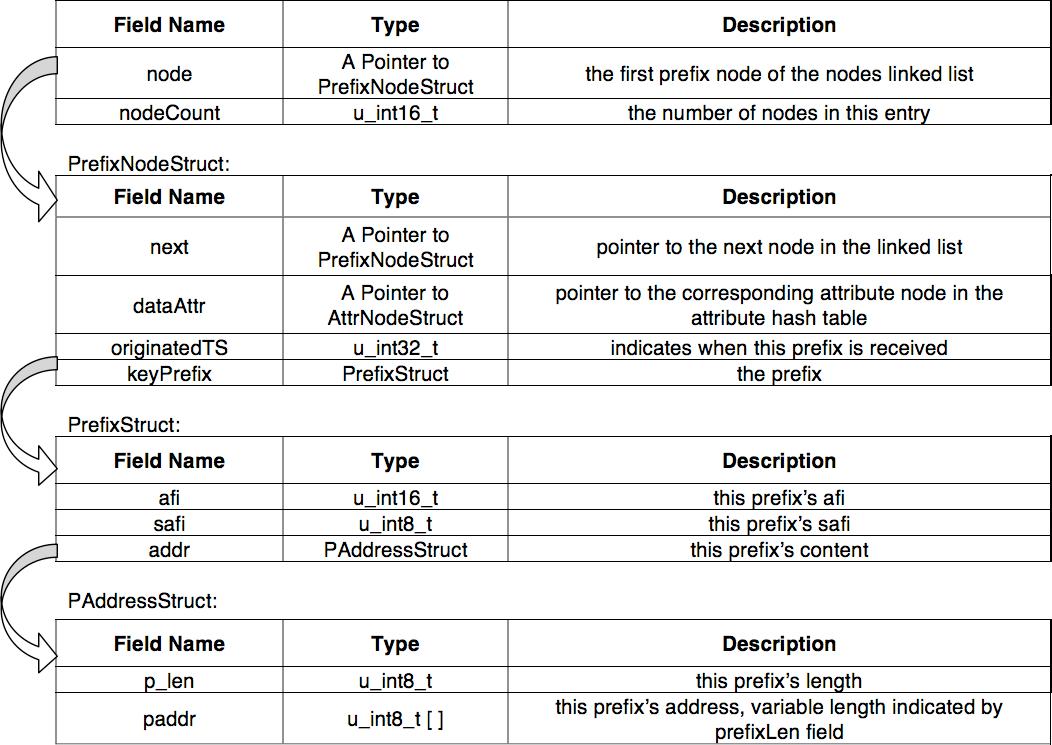
\includegraphics{figs/PrefixEntryStruct.pdf}}
\caption{PrefixEntry Structure}
\label{fig:PrefixEntryStruct}
\end{figure*}
Each prefix in the NLRI of a BGP update will be one node of a particular entry in the prefix table. The index of this entry is calculated by hash value of the prefix. 
2 same prefixes will be hashed to the same entry and stored in the same node.
Because of hash collision, 2 different prefixes could also be hashed to the same entry. But they will be stored in difference nodes of this entry.

\subsubsection{AttributeTable Structure}
\label{sec:labeling:attributetable}
Attribute hash table is similar to the prefix hash table mentioned in the previous section. AttributeTable structure is used to implement a hash table to store the attributes of BGP updates. It has the following six parts.
\begin{itemize}
\item{\emph{attributeCount:} is the number of attributes are contained in the attribute hash table.}
\item{\emph{tableSize:} is the number of entries in the hash table.}
\item{\emph{occupiedSize:} is the number of occupied entries in the hash table. }
\item{\emph{maxNodeCount:} is the max length of all entries in the hash table.}
\item{\emph{maxCollision:} is the max number of nodes one entry is allowed to contain.}
\item{\emph{attrEntries:} is an array of AttrEntry structures. For the details of AttrEntry structure, see Figure \ref{fig:AttributeEntryStruct}.}
\end{itemize}
\begin{figure*}
\centering
\scalebox{1}{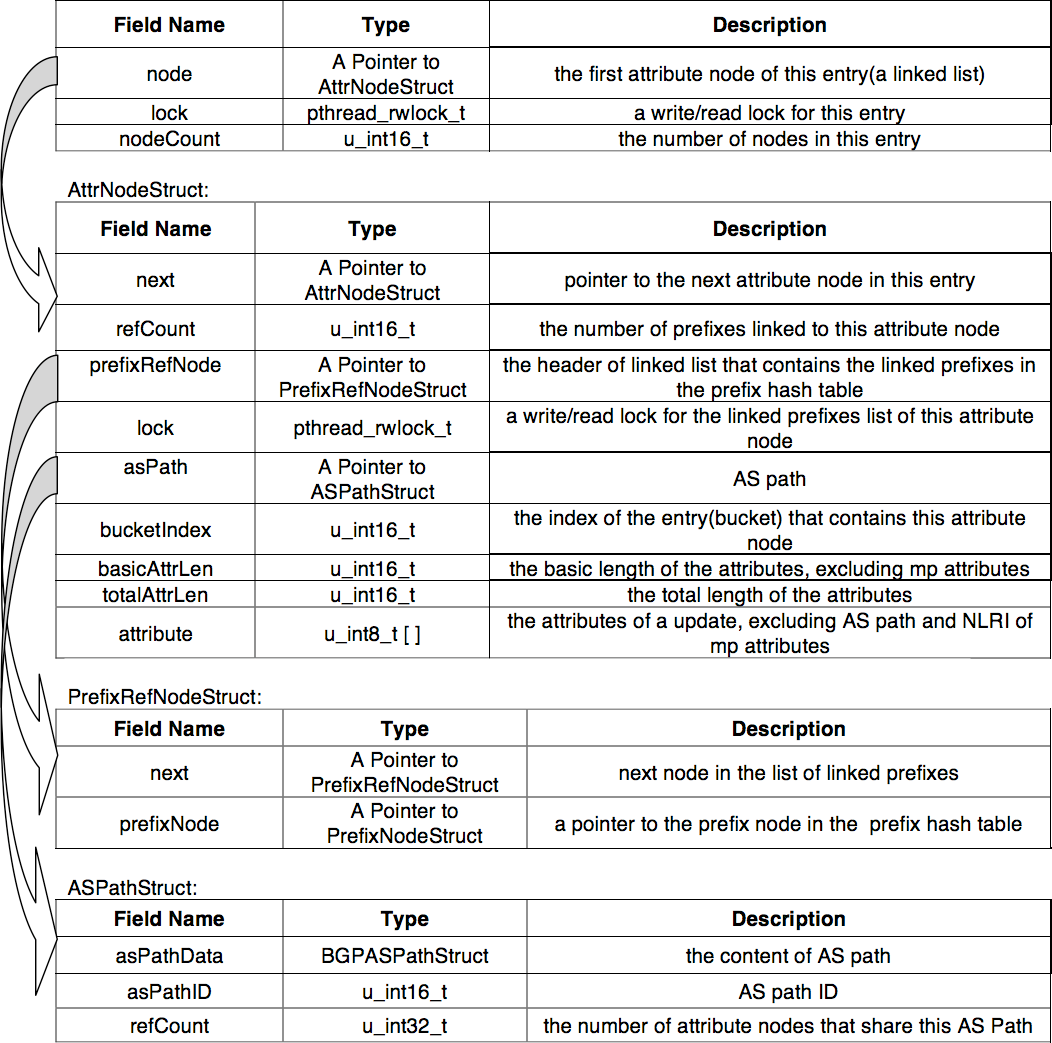
\includegraphics{figs/AttributeEntryStruct.pdf}}
\caption{AttributeEntry Structure}
\label{fig:AttributeEntryStruct}
\end{figure*}
In the attribute table, the attribute set in a BGP update will be stored in one node. And which entry this node belongs to is determined only by the hash value of AS path.
That means if 2 attribute sets have the same AS path, they will be hashed to the same entry. If other attributes of the 2 sets are also same, they will be stored in the same node. 
If 2 attribute sets have the same AS path but other attributes are different, they will still be stored in the same entry but 2 different nodes.  
Note in the case the AS path is only stored once and the 2 different nodes will link to the same AS path.
Again it is possible that  2 attribute sets with different AS paths are hashed to the same entry because of hash collision.

   

\subsection{Main Flow Logic}
\label{sec:labeling:mainflow}
After introducing the data structure, we describe the main flow logic of labeling module here. As we mentioned, labeling module reads the BMF messages from peer queue. For the BMF messages with type other than 2 (see Figure \ref{tab:types}), the labeling module simply writes them into labeling queue without any processing.  For each BMF message with type 2, labeling module processes it as follows:  
\begin{itemize}
\item{If it doesn't contain a BGP update message, simply writes it into labeling queue without any processing.}
\item{If it contains a BGP update message,  extract the session ID from the BMF message. With the sesionID the labeling module finds the peering session structure and checks the 'labelAction' in it (see Figure \ref{fig:configurationSub}).  }
	\begin{itemize}
		\item{If the field 'labelAction' is set to "None", simply writes the BMF message into label queue without any processing.}
		\item{If the field 'labelAction' is set to "RibStore", updates the RIB-IN table of the corresponding peering session and then writes the the BMF message into label queue. In section \ref{sec:labeling:storerib} we will discuss the detail about how to update RIB-IN tables given a BGP update message. }
			\item{If the field 'labelAction' is set to "label", updates the RIB-IN table of the corresponding peering session and labels this BMF message. Specifically, one label for each prefix in NLRI will be attached to the BMF message and its message type will be changed to 3. Finally the new BMF message with type 3 will be written into label queue. In section \ref{sec:labeling:label} we will discuss the detail about how to label a BGP update message.}
	\end{itemize}
\end{itemize}

\subsection{Store RIB-IN Tables}
\label{sec:labeling:storerib}
The labeling module stores RIB-IN tables on a per-peer basis. For each incoming BGP update message from a peer, the labeling module stores it in the peer's RIB-IN table as follows:
\begin{enumerate}
	\item{Parse the BGP update message into the following components:}
	\begin{itemize}
		\item{IPv4 unicast reachable NLRI and unreach NLRI}
		\item{multiple protocol(mp) reachable NLRI and unreach NLRI}
		\item{the attribute set excluding AS path, mp unreachable attributes and NLRI of mp reachable attributes}
		\item{AS path}
	\end{itemize}
	
	\item{Hash the AS path and find the entry in the attribute table based on the hash value. Then check each node of this entry against the AS path and attribute set from above as follows:}
	\begin{itemize}
		\item{If the current node's AS path and attribute set are the same, return this attribute node.}
		\item{If the current node's AS path is same but attribute set is not, return a new created attribute node that has the new attribute set and is linked to the existing AS path. Recall the same AS path shared by multiple nodes is only stored once.}
	\end{itemize}
	\item{If none of the nodes matches the above 2 rules, return a new created attribute node with the new AS path and attribute set.}
		
	\item{Extract all prefixes from IPv4 unicast reachable NLRI and mp reachable NLRI. Each prefix is processed as follows: }
	\begin{itemize}
		\item{If there is a existing prefix node which contains the same prefix content such as such as afi, safi, mask length and address in the prefix hash table:}
		\begin{itemize}
			\item{If the existing prefix node's linked attribute node('dataAttr' field in Figure\ref{fig:PrefixEntryStruct}) is same as the attribute node returned from step 2, do nothing.}			\item{Otherwise:}
			\begin{itemize}
				\item{Delete this prefix node from its current attribute node's linked prefix nodes list. If there isn't any prefix node linked to this attribute node after this deletion, remove this attribute node from the attribute hash table.}
			\item{Add this prefix node to the linked prefix nodes list in the attribute node returned from step 2.}
			\end{itemize} 	
		\end{itemize}
		\item{Otherwise:}
		\begin{itemize}
			\item{Create a prefix node(PrefixNodeStruct, see Figure\ref{fig:PrefixEntryStruct}) based on the prefix's content.}
			\item{The created prefix node is placed into an entry(PrefixEntryStruct, see Figure\ref{fig:PrefixEntryStruct}) in the prefix hash table based on the hash value of the prefix's content.} 			\item{Update its linked attribute node field('dataAttr' field in Figure\ref{fig:PrefixEntryStruct} with the attribute node returned from step 2. }
			\item{As each attribute node maintains a list of all linked prefix nodes, we also need to add this new created prefix node to that list of the attribute node returned from step 2}
		\end{itemize}
	\end{itemize}
	
	\item{Extract all prefixes from the IPv4 unicast unreachable NLRI and multiprotocol unreachable NLRI. Each prefix is processed as follows:}
	\begin{itemize}
		\item{If there is a existing prefix node which contains the same prefix content such as such as afi, safi, mask length and address in the prefix hash table:}
		\begin{itemize}
			\item{Delete this prefix node from its corresponding attribute node's linked prefix nodes list. If there isn't any prefix node linked to this attribute node after this deletion, remove this attribute node from the attribute hash table.}
			\item{Remove this prefix node from the prefix hash table.} 		\end{itemize} 					
		\item{Otherwise: Do nothing.}
	\end{itemize}		
\end{enumerate}


\subsection{Labels the BGP updates}
\label{sec:labeling:label}
The labeling module labels all the prefixes in a BGP update message base on how they change RIB-IN tables. More specifically, the label classifies the prefixes into six categories: 'new announcement' versus 'duplicate announcement', 'same path' versus 'different path' and 'withdraw' versus 'duplicate withdrawal'. In BGP one update consists of multiple prefixes which share the same set of attributes and these prefixes might change the RIB-IN tables in different ways. As a result, the multiple prefixes in one BGP updates have to be labeled separately. That's why labeling has to be done on a per-prefix basis, not a per-update basis.

Labeling is done as follows:
\begin{enumerate}
	\item{Return a existing or new created attribute node according the step 1 and 2 in the preview subsection. }
	\item{Extract all prefixes from IPv4 unicast reachable NLRI and multiprotocol reachable NLRI. Each prefix is labeled as follows: }
	\begin{itemize}
		\item{If there is a existing prefix node which contains the same prefix content such as such as afi, safi, mask length and address in the prefix hash table:}
		\begin{itemize}
			\item{If the existing prefix node's linked attribute node ('attributeNode' field in Figure\ref{fig:PrefixEntryStruct} is same as the attribute node return from step 1, label it as 'duplicate announcement'.}			\item{Otherwise, compare the 'AS Path' in this prefix node's current linked attribute node to the 'AS Path' in the attribute node returned from step 1. }
			\begin{itemize}
				\item{If they are same, label it as 'same path'. }				\item{Otherwise, label it as 'different path'. }
			\end{itemize} 	
		\end{itemize}			    
		\item{Otherwise, label it as 'new announcement'. }
	\end{itemize}
	
	\item{Extract the IPv4 unicast unreachable NLRI and multiprotocol unreachable NLRI. Each prefix is labeled as follows:}
	\begin{itemize}
		\item{If there is a existing prefix node which contains the same prefix content such as such as afi, safi, mask length and address in the prefix hash table, label it as 'withdraw'}		
			\item{Otherwise:  label it as 'duplicate withdraw'.}
	\end{itemize}
\end{enumerate}
	
\subsection{Design Philosophy}
The first design issue here is how to organize a RIB table in memory. Logically a RIB table can be viewed as prefixes and attributes that are interlinked together. And another observation is that a set of attributes is typically shared by multiple prefixes as they are received in one BGP update.  Based on these observations. we decided to store a RIB by using 2 interlinked hash tables: prefix hash table and attribute hash table.
As we discussed in subsecions \ref{sec:labeling:prefixtable} and \ref{sec:labeling:attributetable}, these 2 hash tables has the same structure in a high level. Specifically both of them consists of multiple entries and each entry is a linked list that has multiple nodes. In the prefix hash table each node represents a prefix and in attribute hash table each node holds a set of attributes. And the prefixes and the set of attributes are linked together if they are received in the same BGP update. Note one prefix node representing a single prefix can only be linked to one attribute node holding a set of attributes. But one attribute node could be linked to multiple prefix nodes. In other words, the relationship between prefix node and attribute node is many to one.

The second design issue is how to store the prefixes and the set of attributes in a BGP update efficiently. For a prefix it is straightforward to hash the prefix to an entry(bucket) in the prefix hash table. Then all the nodes of this entry are checked in order to know if this prefix is existing or not. For the set of attributes, we have 2 options here:
	\begin{itemize}
		\item{\emph{Option1: }Hash the entire set of attributes to an entry of attribute hash table.}		
		\item{\emph{Option2: }Extract the AS path form the set of attributes and then hash the AS path to find an entry for the set of attributes.}
	\end{itemize}
Each option has its own pros and cons. Option1 basically hashes each unique set of attributes to a different entry(bucket) if ignoring the hash collision. That will make the attribute hash table too long in terms of the number of entries.
In option2 each set of attributes is assigned to a entry based on the hash value of its AS path. The implication is that all sets of attributes with the same AS path will be assigned to the same entry. As a result, option2 will take fewer entries than needed by option1. But each entry will have more nodes in option2 than option1. So it is a tradeoff between the number of entries and the length of entries.

But besides that option2 is better in comparing the AS paths in 2 sets of attributes. In option2 2 sets of attributes that have different AS paths must be assigned to the different entry. But  2 sets of attributes assigned to the same entry don't necessarily have the same AS path because of hash collision. So when attribute node gets created we tag its AS path with ID in order to differentiate the different AS paths that are assigned to the same entry because of hash collision. As a result, we can compare the AS paths in 2 sets of attributes as follows:
	\begin{itemize}
		\item{If they are assigned to different entries, we know they have different AS paths.}
		     \item{If they are assigned to the same entry, continue to compare their AS Paths' IDs.}
		\begin{itemize}
			\item{If they are the same, we know they have the same AS path.}			
				\item{Otherwise, we know they have different AS paths.}
		\end{itemize}
	\end{itemize}
Contrast to option2, comparing the AS paths in 2 sets of attributes would be more complex in option1 because one first needs to extract the 2 AS paths from them then compare the 2 AS paths in bitwise. That could be a big flaw of option1 as this operation is done for every receiving prefix in BGPmon.

Another advantage of option2 is that all the sets of attributes have the same AS path will share the same AS path structure in memory. In option1 each set of attributes stores the AS path respectively even some of them have the same AS path. So option2 is also better in terms of memory consumption.
Based on all of these, we decided to use option2 in our current design.
 
The last design issue here is about configuration changes. As we mentioned, the only related configure item here is "labelAction" which has 3 values: None, RibStore and Label. All the possible changes are listed:
\begin{itemize}
\item{If "labelAction" changes from Label to RibStore, nothing needs to be done. The labeling module will automatically turn off the labeling fucntion.}
\item{If "labelAction" changes from RibStore to Label, nothing needs to be done. The labeling module will automatically turn on the labeling fucntion.}
\item{If "labelAction" changes from RibStore to None, the RIB table needs to be freed.}
\item{If "labelAction" changes from Label to None, the RIB table needs to be freed.} 
\item{If "labelAction" changes from None to Label, this change cannot be applied immediately. If we apply this change immediately, the labeling will misbehave as we don't have the RIB. For instance, right after the change all the updates labelled as 'new announcement' are actually not new. } 
\item{If "labelAction" changes from None to RibStore,  this change cannot be applied immediately either. If we start to store RIB immediately and right after that user further changes it from RibStore to Label, we will run into the same problem as above. } 
\end{itemize}
The only way to make the last 2 changes applied is to reset the session. When a new session starts, the changes will be applied automatically and labeling will behave correctly.

\section{Periodic Event Handling Module}
\label{sec:periodic}
Periodic event Handling Module(periodic module in short) manages periodic events such as route refresh requests and periodic status messages.
This module has two threads:
\begin{itemize}
%\item{Periodically writes sessions status trigger message (type 3) into label queue if configured.}
\item{\emph{Periodic Status Messages Thread:} It periodically writes session status messages(BMF type 5), queues status messages(BMF type 6) and chains status messages(BMF type 7) into label queue if configured.}
\item{\emph{Route Refresh Request Thread:} It centralized schedules and executes the route refreshes for all the peers if configured. For each peer, there are two possibilities. }
	\begin{itemize}
		\item{If this peer supports route refresh, periodic module will notify peering module to send route refresh request to the peer.}
		\item{If this peer doesn't support route refresh, periodic module will simulate route refresh by sending local stored RIB-IN out.}
	\end{itemize}
\end{itemize}

The main data structure of periodic event handling module has five fields:
\begin{itemize}
%\item{\emph{sessionsStatusTriggerInt:} It indicates the interval of sending sessions status trigger messages. It is set by configuration module and read by periodic module. }
\item{\emph{StatusMessageInterval:} It indicates the interval of sending periodic status messages for peering sessions, queues and chains. It is configured by user. }
%\item{\emph{sessionsStatusTriggerTimer:} It indicates when is the next time to send sessions status trigger message. It is set and read by periodic module. }
\item{\emph{RouteRefreshInterval:} It indicates the interval of requesting route refresh for every peer that is configured for route refresh. It is configured by user }

%\item{\emph{sessions:} It is a pointer to an array of session structures for all the peers. It is set by configuration module and read by periodic module.}
%\item{\emph{RLs:} It is a pointer to an array of rib and labeling structures for all the peers. It is set by configuration module and read by periodic module.}
\item{\emph{labelQueueWriter:} It is used to write messages into the label queue.}
\item{\emph{shutDownFlag:} It is used to signal periodic module to exit. Specifically both threads keep checking this flag, they will quit if it becomes TRUE.}
\end{itemize}
%\item{\emph{routeRefreshes:} It is a array of RouteRefresh structures. Each session(peer) is attached with one RouteRefresh structure. Each RouteRefresh consists of three field.}
%	\begin{itemize} 
%		\item{\emph{sessionID:} It is a 16 bit session identification. It is set by configuration module and read by periodic module.}
%		\item{\emph{routeRefreshInt:} It indicates the interval of route refresh for this session(peer). It is set by configuration module and read by periodic module.}
%		\item{\emph{routeRefreshTimer:} It indicates the next scheduled route refresh time. It is only used by periodic module. }
%	\end{itemize}
%\end{itemize}
%For the details of this structure, see Figure\ref{fig:PeriodicModuleStruct}.
%\begin{figure*}
%\centering
%\scalebox{1}{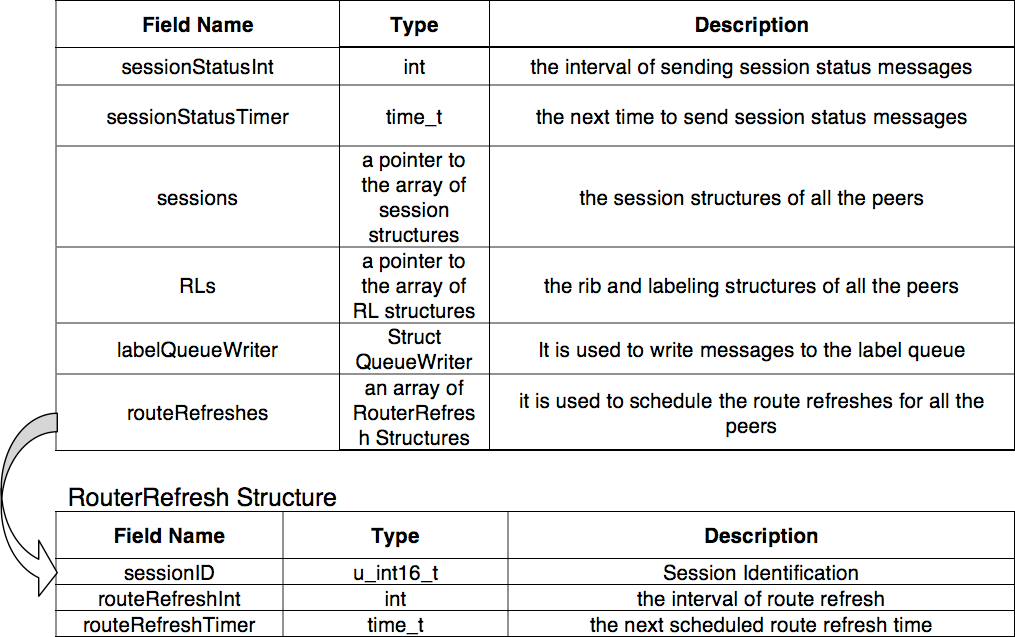
\includegraphics{figs/PeriodicModuleStruct.pdf}}
%\caption{Data Structure of Periodic Event Handling Module}
%\label{fig:PeriodicModuleStruct}
%\end{figure*}
Next we will discuss the detail of the two threads.

\subsection{Periodic Status Messages Thread}
%\subsubsection{ Session Status Message Format}
This thread writes one status message for each peering session, one status message fro all queues and one status message for all chains into the label queue every 'StatusMessageInterval' interval.  Peering session status message (BMF type 5) only includes a session ID instead of including the detail information. Queues' status message(BMF type 6) and chains' status message(BMF type 7) are not associated with a particular peering session.

Then when XML module reads a session status message from label queue, it will extract the session ID from it and retrieve the detail information based on the session ID. Finally the detail information of a peering session will be converted to XML and write into a XML queue. The detail is built from peering session structure( see section \ref{sec:peering:sessionstructure}).  More specifically, it consists of the follow fields:
%\begin{itemize}
%\item{\emph{fsm\_state:} is the current state of FSM that could be one of the six values: Idle, Connect, Active, OpenSent, OpenConfirm and Etablished.  }
%\item{\emph{last\_action:} is a timestamp that indicates when the last action of a peering session is.}
%\item{\emph{establish\_time:} is a timestamp that indicates when the peering session gets established. }
%\item{\emph{message\_rcvd:} is the number of received BGP messages. }
%\item{\emph{prefix\_count:} is the number of prefixes in RIB-IN table. }
%\item{\emph{attribute\_count:} is the number of unique attributes sets in RIB-IN table. }
%\item{\emph{connect\_retry\_count:} is the number of times to retry a tcp connection. }
%\item{\emph{session\_down\_count:} is the number of times BGP session goes down. }
%\item{\emph{session\_last\_down:} is a timestamp that indicated when BGP session went down last time. }
%\end{itemize}
When XML module reads a queues status message from label queue, it will ignore the session ID from it and retrieve the status information all queues. Finally the status information of all peers will be converted to XML and write into a XML queue. Similarly when XML module reads a chains status message from label queue, it will ignore the session ID from it and retrieve the status information all chains.
For the XML format of these periodic status messages, please refer to the XML specification.

%\begin{itemize}
%\item{\emph{FSM Info:} It contains 'state', 'keepaliveInt', 'holdTime', 'routeRefreshType' from FSM substructure in session structure and 'routerRefreshInt' from RouteRefresh Structure. }
%\item{\emph{Session Stats:} It contains all the fields from statistics substructure in session structure.}
%\item{\emph{RIB and Label Stats:} It contains all the stats related fields from RL structure.}
%\end{itemize}
%For the details of session status message, see Figure\ref{fig:SessionStatusStruct}.
%\begin{figure*}
%\centering
%\scalebox{1}{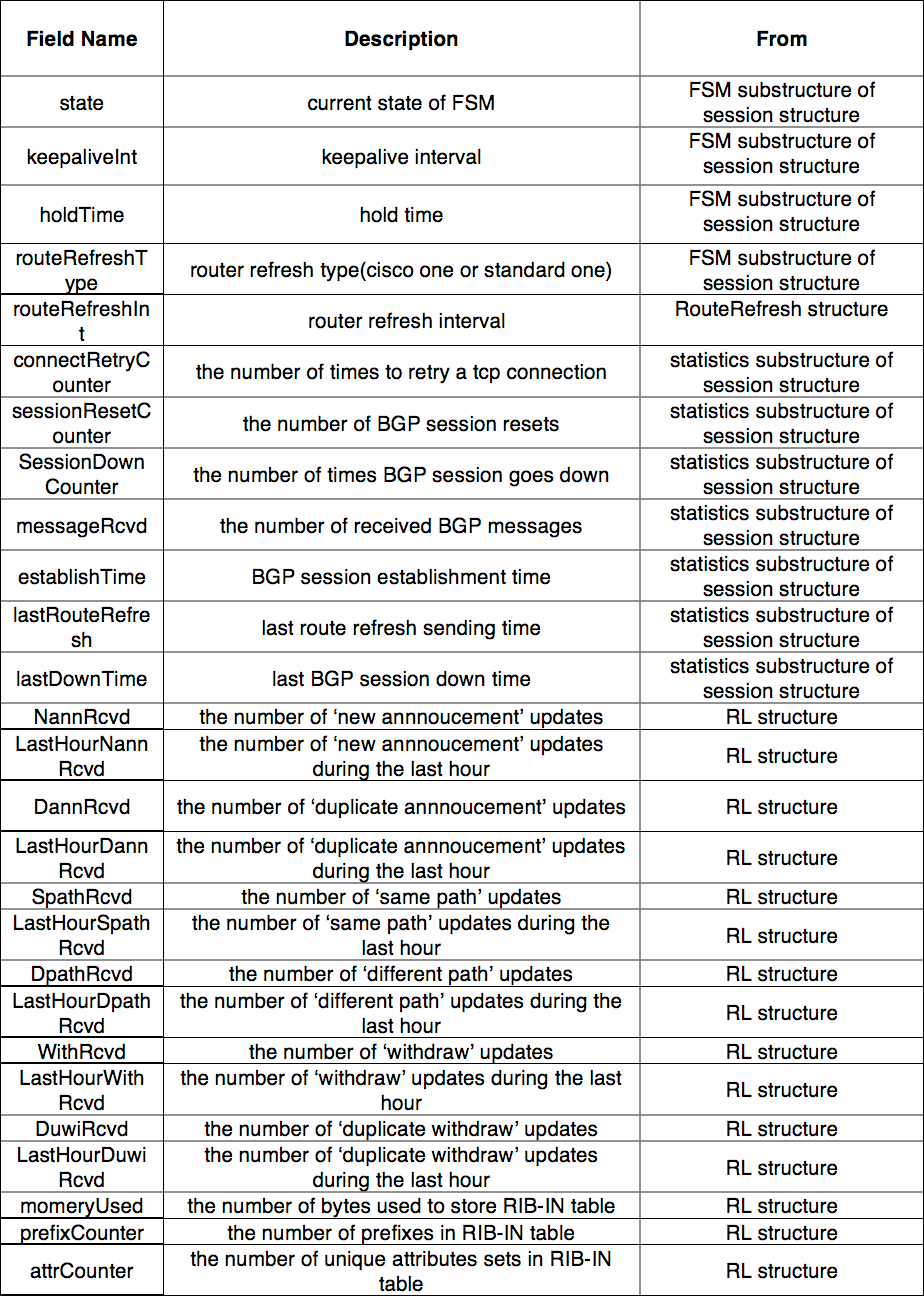
\includegraphics{figs/SessionStatusStruct.pdf}}
%\caption{Data Field of Session Status Message}
%\label{fig:SessionStatusStruct}
%\end{figure*}

%\subsubsection{Send Session Status Messages}

%The 'sessionStatusTimer' field works as a timer to send session status messages for all the peers. When it is timed out, the periodic module will first retrieve all the sessions based on the 'sessions' field in its data structure. Then for each session, the periodic module does the following:
%\begin{itemize}
%\item{Based on its session ID, locate the corresponding RL structure from 'RLs' field in its main data strcutrure.}
%\item{Based on its session ID, locate the corresponding RouteRefresh structure from 'routeRefreshes' field in its main data strcutrure.}
%\item{Create the session status message based on the session ID and current time.}
%\item{Build the data field of created session status message based on the session structure, RL structure and RouteRefresh Structure as we mentioned in the previous subsection. }
%\item{Write this session status message into label queue.}
%\end{itemize}
%If there are several hundreds of sessions, we might want to spread all the session status messages over time evenly in order to avoid a sudden spike in the label queue.

\subsection{Route Refresh Request Thread}
%In our design, the route refreshes for all the peers spread over time evenly in order to avoid overwhelming the queues. 
This thread distributes the route refresh requests for all established peering session evenly over time in order to prevent the queues being overwhelmed.  
%One possible algorithm: 
%\begin{itemize}
%\item{Divide a particular period into several slots. For example, divide 1 hour into 20 slots.}
%\item{Based on the 'routeRefreshes' field, we can know the route refresh interval for each peer. For each peer, we try to find a slot for its first route refresh. }
%\item{If a slot is scheduled by another peer, try the next slot. If all the slots are filled, use the slot with fewest peers. So multiple peers may be scheduled in the same slot.}
%\item{Execute the nearest scheduled route refresh and find a new slot for this peer's next route refresh using the same rules mentioned in the previous step. }
%\end{itemize}

%\subsection{Execute a Scheduled Route Refresh}
If a route refresh request is for one peer that supports route refresh, the periodic module just needs to notify peering module to issue a route refresh request message. Otherwise the periodic module has to simulate a route refresh by sending out this peer's local RIB-IN. The detail of handling the route refresh request for a establish peering session is as follows:
\begin{itemize}
%\item{ Look up the array of session structures which is pointed by 'sessions' field and find this peer's session structure based on its session ID.}
\item{ Check if route refresh is enabled for this session. If not, do nothing. Otherwise, continue. }
\item{ Check the 'routeRefreshType' field of session structure( see section \ref{sec:peering:sessionstructure})..}
	\begin{itemize}
 	\item{if it is 0, that means this peer doesn't support route refresh. The periodic module needs to send out this peer's RIB-IN table as follows:}
			\begin{itemize}
				%\item{Look up the array of RL structures which is pointed by 'RLs' field and find this peer's RL structure based on its session ID.}
				\item{The 'prefixTable' and 'attributeTable' fields of the found RL structure compose this peer's RIB-IN. For each node in the attribute table, do the following things:}
					\begin{itemize}
						\item{Find all the related prefix nodes in the prefix table. }
						\item{Build a BMF message(type 4) that contains a BGP update that is built based on the attribute node and all related prefix nodes.}						
								\item{Write this BMF message into label queue.}
					\end{itemize}	
			\end{itemize}
	  \item{Otherwise, that means this peer supports route refresh. The periodic module just needs to set the 'routeRefreshFlag' field of session structure to TRUE in order to signal the peering module to send out route refresh request to the peer.}
 	\end{itemize}
\end{itemize}

 \subsection{Design Philosophy}
 Actually in the previous design we used to put the logic of sending route refresh requests and periodic status messages in the peering module. 
 More specifically each peering thread decides when to send its own route refresh requests and periodic status messages. 
 But it turns out we lost the ability to schedule these events from a global view. Specially for route refresh requests, it is important to schedule them carefully as each of them will trigger hundreds of thousands of messages that could be a  big burden for the entire system. If all the peers' route refresh request are scheduled at the same time, the queues in BGPmon might not be able to hold the huge amount of messages trigged by them.
 
In the current design, we have a dedicated module to schedule these events. The route refresh requests of all peers are scheduled evenly over the time based based on "RouteRefreshInterval" and the number of peers in order to prevent the queues from being overwhelmed.  In contrast to route refresh requests, the periodoc status messages of all peers are simply written into the label queue every "StatusMessageInterval" as the size of periodic status message is pretty small. But by decoupling the scheduling from peering module it is easy to plug in some sophisticated scheduling algorithms for the periodic status message as needed.
%\subsection{Dynamic Configuration Change}
%In the periodic event handling module, two parts may be changed dynamically by configuration module.
%\begin{itemize}
%\item{\emph{sessionsStatusTriggerInt:} the interval of sending sessions status trigger messages.}
%\item{\emph{routeRefreshInt:} the router refresh interval of each peer.}
%\end{itemize}
%These configuration changes can be automatically adopted when the periodic module sets the time for the next sessions status trigger message and route refresh.
\section{XML Generation Module}
\label{sec:xml}

%The XML thread simply copies from the label queue to the xml queue for processing by the clients.
The XML generation module manages the conversion of all BGPmon received and generated messages into XML. It has one single thread which consists of three main steps. 
\begin{itemize}
\item{It reads messages from the label queue. These messages can be any of all eight types in Figure \ref{tab:types}.}
\item{It converts all types of messages into XML format according to our XML specification. }
\item{It writes messages in XML format to the XML queue for processing by the client threads.}
\end{itemize}

%The main data structure of  XML generation module only consists of two fields.
%\begin{itemize}
%%\item{\emph{expandModeFlag}: It is a 0 or 1 flag. If it is set to 0, the XML generation module will work in normal mode. If it is set to 1, it will work in expand model. We will discuss these two modes later in this secion.
%%If it is set to 0, the session ID field in the internal messages will not be expanded before XML generation. If it is set to 1, the session ID field will be expanded to the status of the session before XML generation. 
%%} 
%%\item{\emph{sessions:} It is a pointer to an array of session structures for all the peers.}
%%\item{\emph{RLs:} It is a pointer to an array of rib and labeling structures for all the peers.}
%\item{\emph{labelQueueReader:} It is used to read the messages from the label queue.}
%\item{\emph{XMLQueueWriter:} It is used to write the converted messages to the XML queue.}
%\end{itemize}


%\subsection{Expanding Session ID}
%In order to expand the session ID before XML generation, the XML generation thread needs to locate all the information related the session status. In our design all the session status information are from session structure(Figure \ref{fig:sessionStruct}) and RL structure(Figure \ref{fig:RLStruct}).
%%More specifically, the XML generation thread extracts the data from session structure and RL structure to build the session status.
%Do we need to discuss the exact format of session status?

%For different types of internal messages read from label queue, session ID expansion works differently.
%\begin{itemize}
%\item{ \emph{Type 1, 2, 4, 7, 8:} If  expandFlag is set to 1, the session ID in them needs to be expanded to the status of the corresponding session before XML generation. In this case, the session status is attached to each message before XML generation. Otherwise they can directly be converted to XML. 

%\item{ \emph{Type 3:} If  expandFlag is set to 0, XML generation module doesn't need to expand the session ID for other types of internal messages. the periodic module will send this type of message periodically. That means  such as 1, 2, 4, 7 and 8. In this case, XML gener 

%\end{itemize}

%\subsection{XML Format Overview}
%The XML formats of all eight types internal messages share the same basic structure as follows:
%\begin{verbatim}
%<bgpmon>
%	<time>...</time>
%	<peering>...</peering>
%	[ <message>...</message> |
%	  <status>...</status> |
%         <state_change>...</state_change> |
%         <start>...</start> |
%         <stop>...</stop>|
%	  <table_transfer_entry>...</table_transfer_entry>]
%   </bgpmon>
%\end{verbatim}

%The 'time' element is the most common part, it has the following three sub elements: 
%\begin{itemize}
%\item{\emph{time:} It is in unix format and converted from 'TimeStamp' in the internal format (see Figure\ref{fig:BMF}).}
%\item{\emph{precision\_time:} It is in unix format and converted from 'PrecisionTime' in the internal format (see Figure\ref{fig:BMF}).}
%\item{\emph{GMT:} It is GMT format and converted from both 'TimeStamp' in the internal format (see Figure\ref{fig:BMF}).}
%\end{itemize}

%The 'peering' element is the common part for all types except types 5 and 6. It has six sub elements:
%\begin{itemize}
%\item{\emph{src\_as:} It is the source AS number. }
%\item{\emph{src\_ip:} It is IPv4 or IPv6 source address.}
%\item{\emph{src\_port:} It is the source port number.}
%\item{\emph{dst\_as:} It is the destination AS number. }
%\item{\emph{dst\_ip:} It is IPv4 or IPv6 destination address.}
%\item{\emph{dst\_port:} It is the destination port number.}
%\end{itemize}
%Note this 'peering' element should be maintained by configuration module. And configuration module should maintain this element for both directions: from peer to monitor and from monitor to peer.
%\begin{itemize}
%\item{\emph{from peer to monitor:} The peer is the source and the monitor is the destination. It is used for type 1,3,4,7 and 8}
%\item{\emph{from monitor to peer:} The monitor is the source and the peer is the destination. It is used only for type 2.}
%\end{itemize}
%The configuration module should be able to provide 'peering' element in string by given session ID and a specific direction.

%Another critical issue is about the changes of 'peering' element. For example after one message $M$ with 'sessionID' 1 are written into the peer queue, the 'scr\_ip' of the 'peering' element of this session changes. Some time later the message $M$ is processed by XML module and XML module will ask configuration module for the 'peering' element with 'sessionID' 1. As a result, the configuration module will provide the 'peering' element with the new 'src\_ip' and this new 'src\_ip' will be used in the final XML format of message $M$. Obviously it is a inconsistency problem. 

%The solution is whenever anyone of the six sub elements changes, the configuration module needs to keep the current session ID and its corresponding 'peering' element unchanged. And it also needs to create a new session ID and a new 'peering' element which includes the changes. Then in the above case, the XML module can still get the old 'peering' element based on the old session ID.

%The remaining part actually is the body of XML message. It uses different elements to represent various types.
%\begin{itemize}
%\item{\emph{message:} It is corresponding to type 1, 2 and 7. By looking at the 'peering' element, we can distinguish between incoming(type 1) messages and outgoing(type 2) messages.}
%\item{\emph{status} It is corresponding to type 3.}
%\item{\emph{state\_change:} It is corresponding to type 4.}
%\item{\emph{start:} It is corresponding to type 5. }
%\item{\emph{stop:} It is corresponding to type 6.}
%\item{\emph{table\_transfer\_entry} It is corresponding to type 8. Its format is same as element 'message'. We only use a different element to identify table transfers.}
%\end{itemize}
%For the details about these elements, please refer to the XML specification.


%\subsection{Convert Internal Messages to XML}
%The XML generation module reads the internal messages in any of the eight types from label queue and converts them into XML as follows:
%%\begin{itemize}
%\item{}
%\end{itemize} 





%\subsection{Expand Mode}
%In expand mode the XML generation module reads the internal messages with types 1, 2, 4, 5, 6, 7, 8 from label queue. 
%\begin{itemize}
%\item{For messages with type 5 and 6, they can be converted directly into XML and writes into XML queue.}
%\item{For messages with type 1, 2, 4, 7 and 8, the session ID in them needs to be expanded to the status of the corresponding session before XML generation. It uses the same approach as normal mode to locate all the information related the session status. The session status is attached to each message before XML generation and then convert them together into XML.}
%In expand mode, type 3 message is not supposed to appear in label queue because the session status is attached to each session related message and the periodically sent session status messages are not needed. But in case the temporary inconsistence between periodic module and XML generation module, the XML generation module should ignore all the messages with type 3 read from label queue. 

%The advantage of expand mode is a client can know the session status of a session related message by just reading the content of this message.  But in this mode, the session related message's size is bigger than normal mode as the session status is included.
%\end{itemize}
\subsection{XML Format Overview}
The XML module converts all the messages from BMF to XFB, a XML-based format for BGP routing information. XML is a general-purpose markup language; its primary purpose is to facilitate the sharing of data across different information systems, particularly via the Internet. Using XML as the base for our XFB markup provides the following advantages:

  \begin{itemize}
  \item{ XFB is human and machine-readable. By using CSS or XSL, XFB can be easily displayed on websites. Because XFB is based on XML which is a common interface to many applications, XFB can be processed by a variety of existing tools. }

   \item{XFB can easily be extended with additional information based on the raw BGP routing information. The BGP data is simply annotated with additional attributes and/or elements; programs which are not looking for this new information will simply ignore it. This allows us to easily modify XFB in general (or particular BGPmons) to allow for newly required information. We include guidelines for adding new standard elements in each section.}

    \item{XFB messages can be used to reconstruct the raw BGP messages, if needed. }
  \end{itemize}
Though XFB pays a storage cost since a compact binary message is (usually) expanded into ASCII text with additional tags, the results of our experiments using the default compression parameters for bzip2 on XFB data are promising.  Currently there are two types of BGP routing information which are included in XFB: BGP messages which come "over the wire" and may or may not have additional "helper" information appended, and BGP control information that originates with the BGPmon. 
For the details about XFB, please refer to the BGPmon XFB specification.

\subsection{Design Philosophy}
%The output format of BGPmon is one critical design issue. As BGP routing information is an essential resource for both researchers and operation communities in Internet routing In order to collect and aggregate this information, it is important to define a public format to encapsulate, export, and archive it. But what are the requirements for this format?

%    * human and machine-readable 

%    * easily accessible 

%    * suitable for further processing by existing tools 

%    * easy to add user annotations 

%    * easy to reconstuct raw BGP messages / ability to replay into router 

%    * record full control information 

%    * support BGP extensions 

There are two issues when we design how to convert messages to xml.
\begin{itemize}
\item{How to convert the fields which are not defined in xml specification?  The answer to this question is each unknown field is represented by the a 'Octets'
   element.  The 'Octets' element looks like: $<$octets length = '3'$>$2E3A4D$<$$/$octets$>$. In this way, we avoid any information loss even for the information we don't know.}
\item{How to convert the xml message back to binary?  Similar to the previous one, the solution is we piggyback a 'Octets' field which represent the entire BGP raw message from wire in the end of xml message. In this way, we can easily replay some BGP raw messages to routers by extracting the last 'Octets' field.  }
\end{itemize} 


%\subsection{Dynamic Configuration Change}
%N/A
%Similar to the other modules,  the XML generation module also needs to detect the dynamic configuration changes related its running mode(normal or expand). In order to detect these configuration changes, the field 'expandModeFlag' in the data structure is set by configuration module and read by XML generation module.
%Right before processing each message from label queue, the XML generation module needs to check the flag and change its running mode.



\section{BGPmon Clients}
\label{sec:clients}


\section{Chain Module}
\label{sec:chains}
This module is used to allow BGPmon to scale out through chaining multiple BGPmons. BGPmons are chained together via tcp connections. Con�guration of BGPmon chains is manual so care must be taken not to create loops in the topology.
One BGPmon could initialize a chain to another BGPmon or accept a chain from another BGPmon. From the perspective of BGPmon accepting a chain, the BGPmon intializing the chain is same as a typical client.  As a result, the logic of accepting a chain and serving data is already handled by clients control module(see section\ref{sec:clients}). 

On another side, Initializing a chain and processing data are implemented in this chain module. 
At the beginning of BGPmon, for each configured chain its data structure is populated and its threads is launched if it is enabled. After that, chains can be created, deleted, disabled and enabled via command line interface(CLI). 
 
\subsection{Data Structure}
The main data structure of a chain has the following fields:
\begin{itemize}
\item{\emph{chainID:} It is the unique identifier of a chain.  It is an integer starting from 0 and automatically assigned when a new chain is created.}
\item{\emph{addr:} It is the address of remote BGPmon.  It is a string which could be a IPv4/IPv6 address or one of two keywords(ipv4loopback and ipv6loopback). After it is intialized from configuration, it could be set via command line interface(CLI) at runtime.}
\item{\emph{port:} It is the listening port of remote BGPmon.  It is an integer.  It also could be set via command line interface(CLI) at runtime after initialization.}
\item{\emph{enabled:} It is a boolean value indicating the status of a chain.  If it is FALSE, the chain thread will exit. It could be set via command line interface(CLI) at runtime after initialization }
\item{\emph{connectRetryInteval:} It is the tcp connection retry interval in seconds. It could be set via command line interface(CLI) at runtime after initialization}

\item{\emph{deleteChain} This flag will be checked after a chain is disabled. If it is TRUE, the chain's data structure will be freed. It is set by via command line interface(CLI).}
\item{\emph{reconnectFlag:} This flag will be checked every time a message is received or periodic check timer expires. Any changes of "addr" or "port"  will set this flag to TRUE. If it is TURE, the existing tcp connection will be torn down and a new tcp connection(with the latest "addr" and "port") will be initialized.}
\item{\emph{lastAction:} It is a timestamp to indicate when is the last action of this chain. It is used to infer the liveness of the chain thread by thread management module. The chain thread keeps update this timestamp when it is alive. If this field hasn't been updated for a while, the thread management module can infer the chain thread is dead. }
\item{\emph{runningFlag:} It is a flag to indicate if the chain thread is running or not. It should be set to FALSE when the chain thread normally exits. }

\item{\emph{socket:} It is the socket of a chain.}
\item{\emph{serrno:} It is socket error code.}
\item{\emph{connectRetryCounter:} It is the number of times of retrying a tcp connection.}
\item{\emph{connectionState:} It is current connection state of a chain. It could be one of these:  chainStateIdle, chainStateConnecting and chainStateConnected.}
\item{\emph{msgHeaderBuf:} It is used to buffer the header(first 100 bytes) of a XML message. With the length field of header, we can figure out how long the XML messages. Then the complete XML message can be read from the socket and written into the XML queue. Basically every message written into XML queue must be a complete XML message with open tag and close tag, not a partial message. Otherwise the XML messages from different chains will be mangled. }

\item{\emph{establishedTime:} It is a timestamp indicating when a chain got connected to remote BGPmon.}
\item{\emph{lastDownTime:} It indicates when is the last down time of tcp connection.}
\item{\emph{resetCounter:} It is the number of tcp connection resets.}
\item{\emph{messageRcvd:} It is the number of received XML messages via a chain.}

\item{\emph{periodicCheckInt:} It indicates how often the periodic check timer expires.}
\item{\emph{xmlQueueWriter:} It is used to write xml messages to XML queue.}
\end{itemize}
This data structure is attached to each chain thread.

\subsection{Chain Thread}
Each chain is a separate thread and has the following tasks:
\begin{itemize}
\item{ Initialize a tcp connection to a configured remote BGPmon instance(sending side of the chain). }
\item{ Read the XML stream via the tcp connection, cut the stream into messages and write the messages into XML queue. }
\item{ Check the 2 flags: "enabled" and "reconnectFlag" every time a XML message is received or periodic check timer expires .}
	\begin{itemize}
		\item{ The "enabled" flag is set directly by CLI. When it is TRUE, the client thread will exit by itself and if the "deleteChain" flag is also TRUE its corresponding data structure will be freed. }
		\item{ The "reconnectFlag" is also set by CLI. Any changes of "addr" and "port" will set this flag TRUE. If it is TURE, the existing tcp connection will be torn down and a new tcp connection will be initialized with the latest  "addr" and "port".}
	\end{itemize}	
\end{itemize} 

\subsection{Chain Management}
Chains management is done via command line interface(CLI). There are 4 possible chain operations. 
\subsubsection{Create a Chain}
Creating a chain is a synchronous operation. It will occur immediately after function "createChain" is called by CLI. It consists of 2 steps:
\begin{itemize}
\item{ Populate the new chain's data structure. }
\item{ Launch a thread for the new chain if its initial 'enabled' flag is TRUE. }
\end{itemize} 

\subsubsection{Enable a New Chain}
Enabling a chain is a synchronous operation. A new thread will be immediately launched after function "enableChain" is called by CLI. Note the chain's data structure must be existing when the function "enableChain" is called.

\subsubsection{Disable a New Chain}
Disabling a chain is a asynchronous operation. It will NOT occur immediately by calling function "disableChain" by CLI. The function "disableChain" only sets the flag "enabled" to FALSE.
The chain thread will actually exit when a new XML message is received or periodic check timer expires. The difference between disabling a chain and deleting a chain is that disabling a chain will not free the chain's data structure. 

\subsubsection{Delete a Chain}
Deleting a chain is a asynchronous operation. It will NOT occur immediately by calling function "deleteChain" by CLI. Inside the function "deleteChain", both "enabled" flag and "deleteChain" flag are set to TRUE.
The actual actions of exiting chain thread and freeing chain data structure are deferred to the next time a new XML message is received or periodic check timer expires.

\subsection{Design Philosophy}
If one downstream BGPmon is chained to multiple upstream BGPmons, the fundamental design issue is about how downstream BGPMon avoids to mingle the XML streams from upstream BGPmons. 
Remember all the XML streams from upstream BGPmons are mixed together into one stream at the downstream BGPmon by writing them into XML queue.  That means the downstream BGPmon has to first divide the streams from upstream BGPMons into messages and then write all the messages into the XML queue.

We add a length field for each XML message in order to help BGPmon divide stream into messages by giving it a hint about how long the message is. More specifically, downstream BGPmon repeats the following steps to process a stream:
	\begin{itemize}
		\item{ Reads the first a few bytes from stream and figures out the length of the current message }
		\item{ Extracts the message from the stream based on the length from the previous step}
		    \item{ Move the cursor to the end of the current message.}
	\end{itemize}



\section{Queue Module}
\label{sec:queue}
Queue is a utility module which is used by other modules to send messages from one to another. As shown in Figure \ref{fig:architecture}, there are 3 queues in BGPMon.
\begin{itemize}
	\item{\emph{ Peer Queue:} It is used by peering module to send internal messages with type 1,2,4 and 6 to the rib and labeling module.}
	\item{\emph{ Label Queue:} It is used by rib and labeling module, periodic module and main module to send all eight types of internal messages to XML generation module. }
	\item{\emph{ XML Queue:} It is used by XML generation module to send XML messages to client management module which in turn sends them to client applications.}
\end{itemize} 
Each of them is a running instance of queue module. They are created by main module during the initial phase of BGPmon and then used by other modules.

The queue module is build on a circular array and each item in this array contains a generic pointer which points to the real message. In this way we can make queue module generic enough to hold all kinds of messages. It also keeps track all the readers and writers. The main data structure of queue module will be introduced in subsection \ref{sub:queue:struct}.

The queue module implements a Readers/Writers pattern where multiple threads may access the same queue simultaneously, some reading and some writing. We call the reading thread reader and the writing thread writer. Each message written by a writer is available to all the readers and a message can be deleted from the queue only after all the readers read it. A key design issue is the locking mechanism to synchronize access to the share data structure in the queue among all threads.  The details of thread synchronization will be discussed in subsection 
\ref{sub:queue:sync}.
 
The biggest challenge in the design of queue module is to avoid being overwhelmed with limited queue length.  There are two situations we need to address: 1) writers write too fast, and 2) Readers read too slow. We will discuss how to address these two situations in subsection \ref{sub:queue:control}.
 
 
\subsection{\label{sub:queue:struct}{Main Data Structure}}
The main data structure of queue module is called 'Queue'. It consists of four parts:
\begin{itemize}
	 \item{\emph{ General Substructure:} It holds the general information for this queue such as the queue's name, its mutex lock and some logging information. See the details in \ref{sub:queue:struct:general}.}
	\item{\emph{ Items Substructure:} It contains all the data of the queue. It implements a circular array. See the details in \ref{sub:queue:struct:items}.}
	\item{\emph{ Readers Substructure:} It contains the information of all readers of the queue. For example, the sequence number of the next unread item for each reader needs to be maintained here. See the details in \ref{sub:queue:struct:readers}.}
	 \item{\emph{ Writer and Pacing Substructure:} It is used to track all the writers in order to pace them when needed. And some other information needed for pacing are also included here such as pacing on/off threshold.  See the details in \ref{sub:queue:struct:writers}.}
\end{itemize}  

\subsubsection{\label{sub:queue:struct:general}{General Substructure}}
The general substructure has the following fields:
\begin{itemize}
	\item{\emph{name:} It is the name of the queue. In BGPmon, the name of peer queue is 'PeerQueue', the name of lable queue is 'LabelQueue' and the name of XML queue is 'XMLQueue'. }
	\item{\emph{ queueLock:} It is a pthread mutex lock which is used for thread synchronization.}
	\item{\emph{ queuecond:} It is a pthread condition variable which is used to notify a reader when the new item gets wrote.}
	\item{\emph{ logging related fields:} A group of logging related fields such as the historical max number of messages, the historical max number of readers and the historical max number of writers.}
	\end{itemize}
Figure \ref{fig:queue:struct:general} shows the details.
\begin{figure*}
\centering
\scalebox{1}{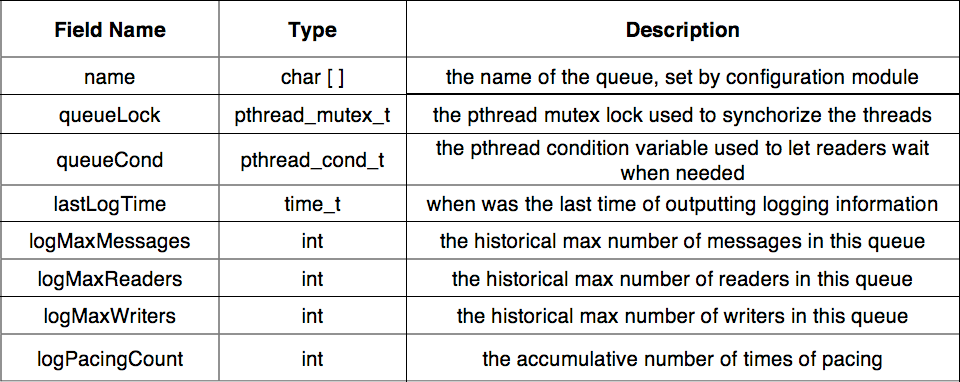
\includegraphics{figs/QueueStructGeneral.pdf}}
\caption{ General Substructure of Queue}
\label{fig:queue:struct:general}
\end{figure*}
	 

\subsubsection{\label{sub:queue:struct:items}{Items Substructure}}
Items substructure maintains a circular array of items which is the heart of queue module. 
Each item is defined as a 'QueueEntry' structure which has the following two fields:
\begin{itemize}
	\item{\emph{count:} It indicates how many readers haven't read it.   This reference count decrements by one after one reader reads this item. If the reference count of a item is zero, this item can be reclaimed by the queue module. Otherwise this item cannot be reclaimed.}
	\item{\emph{messageBuf(void *):} It points to the real data buffer of this item. The data buffer must be created by writers and be passed into queue module.}
\end{itemize}
Items substructure has the following five fields:
\begin{itemize}
	  \item{\emph{head:} It is the sequence number of the oldest item in the queue. It means at least one reader hasn't read this item. The 'head' is incremented after the oldest data item is read by the last reader. }
	  \item{\emph{tail:} It is the sequence number of the next available item in the queue. It is incremented by writing a new message into the queue. }
	  \item{\emph{items:} It is an array of items. Each item is a 'QueueEntry' structure.}
	  \item{\emph{ copy:} It is a callback function. If a reader reads a item and it is not the last reader for this item, the callback function will be called to return a copy of this item to the reader. If a reader is the last one of a item, this item will be returned directly. This allows the reader to always free the returned item after processing it without knowing the details of queue. }
	  \item{\emph{ sizeof:} It is a callback function. Based on 'QueueEntry' structure, we know the size of a item depends the size of its data buffer. This function is used to get the size of a data buffer in bytes. As the data format is queue specific, the sizeof function is provided by the queue creator.}
\end{itemize}
In order to avoid drop any messages in the queue, the different between 'head' and 'tail' must be smaller than 'max' field. Note 'head' and 'tail' are all sequence numbers, not subscripts of array. A sequence number(seq) is long integer and is a logical subscript of the queue. The subscript to access the physical array can be calculated by seq \% max.
Figure \ref{fig:queue:struct:items} shows the details of this substructure.
\begin{figure*}
\centering
\scalebox{1}{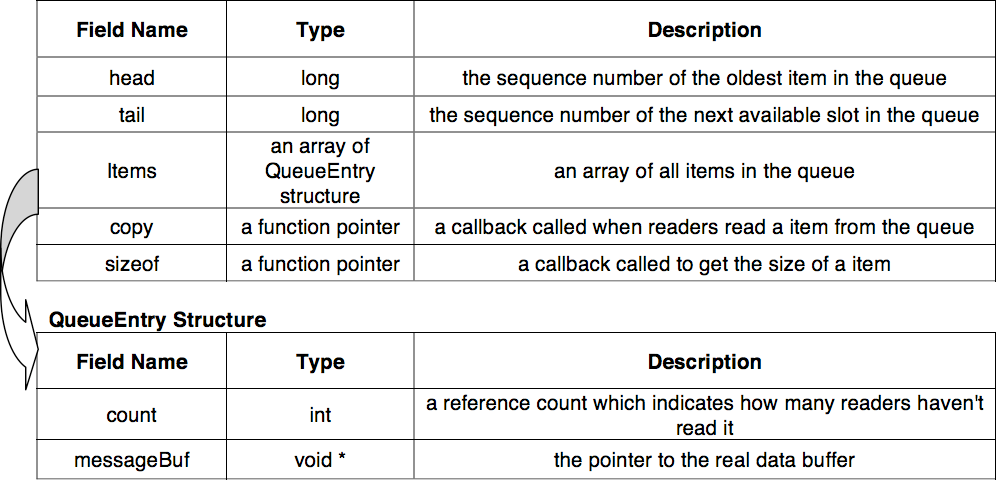
\includegraphics{figs/QueueStructItems.pdf}}
\caption{ Items Substructure of Queue}
\label{fig:queue:struct:items}
\end{figure*}
	 

\subsubsection{\label{sub:queue:struct:readers}{Readers Substructure}}
This substructure is used to track all the readers. It has the following three fields:
\begin{itemize}
	\item{\emph{readerCount:} It is the current number of readers. }
	\item{\emph{nextItem:} It is an array of sequence numbers for all the readers. This array is indexed by reader ID and each sequence number indicates the next unread item in the queue for the corresponding reader. For example, nextItem[6] is the sequence number of the next unread item for the reader with ID 6. The length of this array equals the max number of readers. }
		\item{\emph{itemsRead:}  This array is indexed by reader ID and each element indicates total items read by the corresponding reader. For example, itemsRead[6] is the number of total read items by the reader with ID 6. The length of this array also equals the max number of readers. }
\end{itemize}	
Note the readers of the same queue might have different next item. 


Figure \ref{fig:queue:example} shows an example of the queue which can help us understand the items substructure and readers substructrure.
\begin{figure}[!htb]
\centering
\scalebox{0.44}{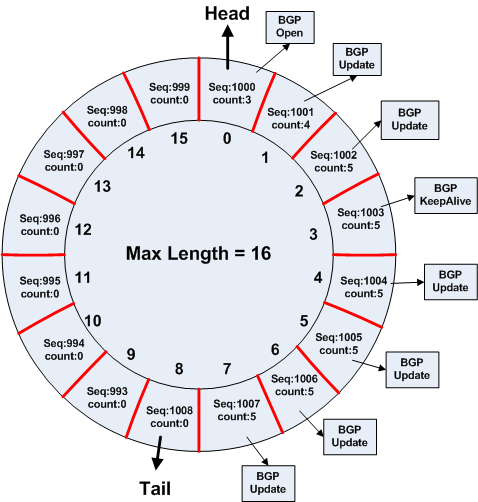
\includegraphics{figs/QueueExample.png}}
\caption{ An Example of Queue}
\label{fig:queue:example}
\end{figure}
In this example, there are a queue with max length 16 and 5 readers. The items substructure looks like this:
\begin{itemize}
	\item{\emph{head:} is 1000 which is sequence number of the oldest item. The count of that item is 3 which means there are three readers haven't read it. }
	  \item{\emph{tail:} is 1008 which is sequence number of the next available item for the new message. }
	  \item{\emph{items:} It is an array of 16 items. 8 of them are in use. }
	  \begin{itemize}
	  	\item{The item with sequence number 1000 has a reference count as 3 which means 3 readers haven't read it.}
		 \item{The item with sequence number 1001 has a reference count as 4 which means 4 readers haven't read it.}
		 \item{All the others item with sequence number from 1002 to 1007 has a reference count as 5 which means all 5 readers haven't read it.}
	\end{itemize}
\end{itemize} 

The corresponding readers substructure is as follows:
\begin{itemize}
	\item{\emph{readerCount:} is 5 which means there are 5 readers.}
	  \item{\emph{nexItem[0]:} is 1000 which means the next item for the reader 0 is 1000 .}
	   \item{\emph{nexItem[1]:} is 1000 which means the next item for the reader 1 is 1000 .}
	    \item{\emph{nexItem[2]:} is 1000 which means the next item for the reader 2 is 1000 .}
	     \item{\emph{nexItem[3]:} is 1001 which means the next item for the reader 3 is 1001 .}
	      \item{\emph{nexItem[4]:} is 1002 which means the next item for the reader 4 is 1002 .}
	      
	     	  \item{\emph{itemsRead[0]:} is 0 which means reader 0 hasn't read anything .}
	   \item{\emph{itemsRead[1]:} is 0 which means reader 1 hasn't read anything.}
	    \item{\emph{itemsRead[2]:} is 0 which means reader 2 hasn't read anything.}
	     \item{\emph{itemsRead[3]:} is 1 which means reader 3 has read 1 items.}
	      \item{\emph{itemsRead[4]:} is 2 which means reader 4 has read 2 items.} 
\end{itemize} 


\subsubsection{\label{sub:queue:struct:writers}{Writers and Pacing Substructure}}
This structure is used to track the writing rate of all the writers and pace them when needed. It has the following fields:
 \begin{itemize}	
 	\item{\emph{writerCount:} It is the number of current writers.}
	  \item{\emph{tick:} It is the start time of the current pacing interval.}
	  	\item{\emph{readCount:} It is used together with 'tick' to count how many messages are read in one interval by all the readers. }
	\item{\emph{writeCounts:} It is an array of counts for all the writers. One count is for each writer which is used together with 'tick' to count how many messages are written in one interval. The length of this array equals the max number of writers.}
	\item{\emph{writesLimit:} It is how many messages are allowed to be written in the queue by each writer in one interval when pacing is turned on. }
	\item{\emph{pacingFlag:} It is set to TRUE if pacing is turned on. It is set to FALSE if pacing is turned off.} 
\end{itemize} 
Figure \ref{fig:queue:struct:writers} shows the details of this substructure.
\begin{figure*}
\centering
\scalebox{1}{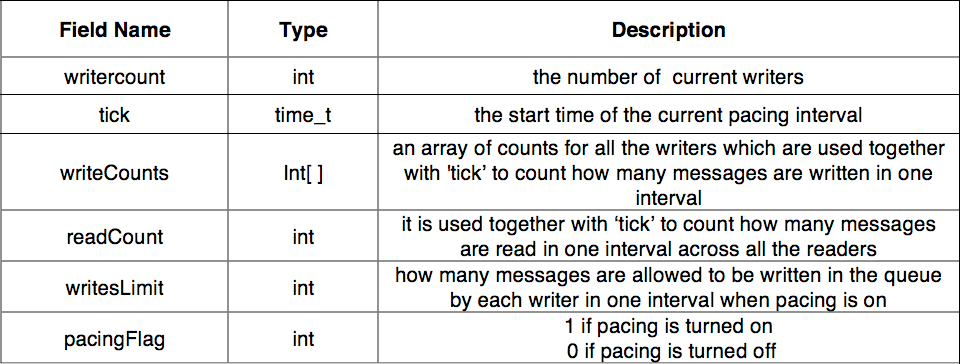
\includegraphics{figs/QueueStructWriters.pdf}}
\caption{ Writers and Pacing Substructure of Queue}
\label{fig:queue:struct:writers}
\end{figure*}
In the subsection \ref{sub:queue:control}, we will discuss how pacing works by using this substructure in detail.
 
\subsection{\label{sub:queue:sync}{Thread Synchronization}}
In BGPmon, there are multiple writers that write messages into one queue and multiple readers that read messages from the same queue. As each read/writer is a separate thread, the thread synchronization is very important for the queue. In our design we use mutex lock and condition variable to manage the thread synchronization. Basically the writer needs to lock the queue by obtaining 'queuelock' in general substructure before it writes a message and unlock the queue by release  'queuelock'  after it writes a message. Similarly the reader needs to lock the queue before it reads a message and unlock the queue after it reads a message.

When a reader exhausts the messages in the queue, it must wait for new messages while other readers or writers still need to continue their reading or writing. In our design, if a reader wants to read a message from the queue and successfully locks the queue by obtaining 'queuelock', it will do the following checks:
 \begin{itemize}	
 	\item{If there are some new messages available for it to read, it will read the oldest one and unlock the queue.}
	\item{Otherwise, it unlocks the queue and waits on the condition variable 'queueCond' to lock the queue again. If any writer writes any new messages into the queue, the queue will broadcast this condition to all the waiting readers.}
\end{itemize} 

\subsection{Interface Functions}
In the queue module, there are only two interface functions which can be used by other modules.
 \begin{itemize}	
 	\item{\emph{readQueue:} It is used to read a message from queue by giving a queue ID, reader ID and a pointer which points to the result data buffer. The return value of 'readQueue' is the number of remaining messages of this reader. It may return READER\_SLOT\_AVAILABLE if this reader has ceased. See details in \ref{sub:queue:control:adjust}}.
	\item{\emph{writeQueue:}  It is used to write a message into queue by giving a queue ID, writer ID and a pointer which points to the written message. It returns 0 if successes.}
\end{itemize}  

\subsection{\label{sub:queue:control}{Stream Control}}
In our design, the queue removes a message until all the readers read it. As a result there are two things we can do in order to prevent a queue being overwhelmed.
\begin{itemize}
	\item{\emph{Pacing writers:} The queue paces the writers according to the average reading rate across all the readers. For example the queue is almost full and there are 4 readers and 2 writers. If each of reader can read 8 messages per second averagely, we should limit the writing rate of each writer to 8/2 = 4 in order to avoid overwhelm the queue.  See details in \ref{sub:queue:control:pacing}.}
	\item{\emph{Adjust slow readers:} In some cases pacing writers doesn't work, the queue needs to adjust the slow readers. For example, the queue is almost full and there are 4 readers and 2 writers. If 3 of the 4 readers can read 8 messages per second but one of them can only read 2 message per second. As a result, the average reading rate across the 4 readers is 6.5 messages per second. In this case, even pacing is turned on and each writer is limited to write 6.5/2 = 3.25 messages per second the queue will still be overwhelmed because the slowest reader cannot read 3.25 messages per second. That's why in this case the queue has to adjust the slowest reader by skipping its unread items. See details in \ref{sub:queue:control:adjust}.}
\end{itemize} 

\subsubsection{\label{sub:queue:control:pacing}{Pacing Writers}}
In our design, the queue utilization(from 0\% to 100\%) is used to determine when to turn on pacing.  When the queue utilization exceeds a configurable threshold(PacingOnThreshold), pacing is turned on until the queue utilization drops below a configurable threshold(PacingOffThreshold).  The reason why we have two thresholds here is this allows the queue to reach a steady state rather than oscillate in and out of pacing.
During the pacing period, the objective is to make the writers write at a pace that matches the average reader. More specifically, in each configurable interval(PacingInterval) the queue limits the number of writes from each writer according to the average number of reads by all readers. 
In order to do this,  when a new interval starts we need to predict the number of reads by all readers in this new interval and then use this value to pace the writers in this new interval.   
The pacing related logic related to the 'readQueue' function is as follows:
\begin{enumerate}
	\item{Check if a new interval starts}
		\begin{enumerate}
		\item{If yes,  update the 'writesLimit' using exponential weighted moving average(EWMA):}
				\begin{enumerate}
					\item{Calculate the new 'writesLimit' by this formula. Note 'alpha' is configurable, 'writesLimit' is the number if writes allowed per writer in the new interval, 'averageReads' is the average number of reads by all readers in the past interval and 'writerCount' is the number of writers.}						
								\begin{eqnarray*}
writesLimit&=& (1-alpha) * writesLimit + \\ 
alpha *  \frac{averageReads}{writerCount}
						\end{eqnarray*}
						\item{If new 'writesLimit' is larger than half of the remaining queue, use half of the remaining queue as the new 'writesLimit'. }
					\item{If new 'writesLimit' is smaller than a configurable 'minWritesLimit', use 'minWritesLimit' as the new 'writesLimit'. }
				\end{enumerate}
		\item{Otherwise, do nothing.}
		\end{enumerate}
		\item{Check if needs to turn off pacing by compare the queue utilization with the configurable threshold(PacingOffThreshold).}
		\begin{enumerate}
			\item{If the queue utilization is smaller, set the 'pacingFlag' field as FALSE. }
			\item{Otherwise, do nothing.}
		\end{enumerate}
\end{enumerate}
Note this logic will be executed every time a reader calls 'readQueue'.

The 'writeQueue' function starts with the same pacing related logic as 'readQueue'. But after that, it needs to limit the number of writes per interval according to the 'writersLimit' field when pacing is enabled. This additional step inside the 'writeQueue' function is as follows:
\begin{enumerate}	
	\item{Check if needs to turn on pacing by compare the queue utilization with the configurable threshold(PacingOnThreshold).}
			\begin{enumerate}
			\item{If the queue utilization is larger, set the 'pacingFlag' field as TRUE. }
			\item{Otherwise, do nothing.}
			\end{enumerate}
			
	\item{Check if 'pacingFlag' is set to TRUE. }
		\begin{enumerate}
		\item{If yes,  do the following checks:}
				\begin{enumerate}
					\item{If 'writeCount[writerID]' is larger than 'writesLimit', sleep until a new interval starts.}
					\item{Otherwise, do nothing.}
				\end{enumerate}									
		\item{Otherwise, do nothing.}
		\end{enumerate}
\end{enumerate}
This logic will be executed every time a writer calls 'writeQueue'.
  
\subsubsection{\label{sub:queue:control:adjust}{Adjust Slow Readers}}
Pacing prevents the queue from being overwhelmed if the readers are uniformly able to read the messages at the same rate.  In the case of a slow reader, the queue utilization will still continue to grow.  When the queue utilization reaches the maximum, the responsible reader is adjusted by skipping all its unread items.
This logic is mainly implemented in the 'writeQueue' function.
\begin{enumerate}
	  \item{Check if the queue is full.}
	     \begin{enumerate}
	     \item{If it is full, find the slowest reader and adjust it by skipping all its unread items. For each reader, check the nextItem[readerID] as follows:}
	     		\begin{enumerate}
	     			\item{ If nextItem[readerID] equals to 'head', adjust this reader as mentioned.}
			\end{enumerate}	
	     \end{enumerate}
\end{enumerate}

In the 'readQueue' function, suppose the queueID, readerID and a pointer is passed in from a caller.
\begin{enumerate}
	\item{If head <= nextItem[readerID] < tail , pass the oldest message to the caller via the pointer and return the number of remaining messages.}
	\item{If nextItem[readerID] >= tail,block the caller until a new message is written into the queue. }
	\item{If nextItem[readerID] = READER\_SLOT\_AVAILABLE , it means the reader has ceased and return READER\_SLOT\_AVAILABLE to the caller.}
\end{enumerate}
If a caller receives READER\_SLOT\_AVAILABLE from 'readQueue', that means the corresponding reader has ceased. Then the caller may need to close thread and release resources in this case.

\subsection{Design Philosophy}
The most important design issue here is how to handle slow readers.  As we discussed, it is essential that some action be taken to address the problem of slow readers. If no action is taken,  a slow reader can cause the queue to overflow and eventually data would be dropped.   This is particularly problematic if most readers could read at a high rate and receive all the data, but a few slow readers fill the queues and cause data loss.   

In the previous design, our solution is to identify and then terminate the slow readers.  However, by doing that a potential problem is that the slow reader may simply re-connect and thus drive the overall system into a state of persistent oscillation.    The system runs well until the slow reader joins.   The slow reader then causes queues to build up and the reader is eventually killed.   The queue then quickly drains when the slow reader is killed.   Note that the queue contains at least one update that has been read by everyone except the slow reader.    When the slow reader is killed, that update can be discarded.    In our experiments thus far, a typical slow reader has hundreds of updates that are waiting only for the slow reader;  killing the slow reader immediately removes these updates and frees hundreds of slots in the queue.   But oscillation occurs if the slow reader immediately connects.    The queue of unread updates begins to build again as soon as the slow reader joins and the cycle repeats.   One can easily imagine a poorly written slow reader that automatically reconnects anytime it is disconnected.

An alternate approach is to better manage, but not kill the slow readers.   In current design, the slow reader is not deleted from the system.   Instead, slow readers are forced to skip messages.     From a queuing standpoint, the effect is similar to killing the slow reader and works as follows.   When BGPmon determines a reader is reading messages too slowly,  all messages that have yet to be read by that slow reader are immediately marked as read.    In this case the slow reader misses several messages, but it is allowed to continue. 




\section{Login Module}
\label{sec:login}

The login module handles the Cisco-like commands typed by logined users and calls the corresponding functions provided by other modules. It is made up of several pieces.  

The first piece is a listener that listens on a specific address and port for new Command Line Interface (CLI) connections.  Once a connection has been established then the next major piece, the command tree structure, is used.  This structure is a tree ADT that contains a complete mapping of all the commands that can be called from the CLI.  Each command is broken down into parts and each part is added to the tree.  For instance the command 'show running' is broken into two pieces.  The 'show' command is a child of the root node and the 'running' command is child of the 'show' command.  When a command is executed from the CLI, the command is sent from the client to the server then broken down and mapped into the command structure.  If the entire command can be mapped onto the tree then the final node will contain a function pointer for the command.  Every node in the structure also has an associated mask with it that controls whether the command is visible or executable to a given security level.  All the commands have been organized in a way that will help make maintenance of them easier.  In commandprompt.c there are a series of functions that contain the necessary code to create the commands and associations to the necessary functions.  Then, there is a series of files that end with '\_commands.c' which contain the functions for each module that the commands reference.
%\section{Summary}
\label{sec:conclude}



\section{Acknowledgements}
\label{sec:ack}




\bibliographystyle{abbrv}
\bibliography{sigproc}

%\appendix

\end{document}
